% Tell RStudio that weaving is to be done with the knitr package
% !Rnw weave = knitr


%\listfiles                   %% Show all files used in the book
\documentclass[10pt,krantz2]{krantz}\usepackage[]{graphicx}\usepackage[]{color}
%% maxwidth is the original width if it is less than linewidth
%% otherwise use linewidth (to make sure the graphics do not exceed the margin)
\makeatletter
\def\maxwidth{ %
  \ifdim\Gin@nat@width>\linewidth
    \linewidth
  \else
    \Gin@nat@width
  \fi
}
\makeatother

\definecolor{fgcolor}{rgb}{0.345, 0.345, 0.345}
\newcommand{\hlnum}[1]{\textcolor[rgb]{0.686,0.059,0.569}{#1}}%
\newcommand{\hlstr}[1]{\textcolor[rgb]{0.192,0.494,0.8}{#1}}%
\newcommand{\hlcom}[1]{\textcolor[rgb]{0.678,0.584,0.686}{\textit{#1}}}%
\newcommand{\hlopt}[1]{\textcolor[rgb]{0,0,0}{#1}}%
\newcommand{\hlstd}[1]{\textcolor[rgb]{0.345,0.345,0.345}{#1}}%
\newcommand{\hlkwa}[1]{\textcolor[rgb]{0.161,0.373,0.58}{\textbf{#1}}}%
\newcommand{\hlkwb}[1]{\textcolor[rgb]{0.69,0.353,0.396}{#1}}%
\newcommand{\hlkwc}[1]{\textcolor[rgb]{0.333,0.667,0.333}{#1}}%
\newcommand{\hlkwd}[1]{\textcolor[rgb]{0.737,0.353,0.396}{\textbf{#1}}}%

\usepackage{framed}
\makeatletter
\newenvironment{kframe}{%
 \def\at@end@of@kframe{}%
 \ifinner\ifhmode%
  \def\at@end@of@kframe{\end{minipage}}%
  \begin{minipage}{\columnwidth}%
 \fi\fi%
 \def\FrameCommand##1{\hskip\@totalleftmargin \hskip-\fboxsep
 \colorbox{shadecolor}{##1}\hskip-\fboxsep
     % There is no \\@totalrightmargin, so:
     \hskip-\linewidth \hskip-\@totalleftmargin \hskip\columnwidth}%
 \MakeFramed {\advance\hsize-\width
   \@totalleftmargin\z@ \linewidth\hsize
   \@setminipage}}%
 {\par\unskip\endMakeFramed%
 \at@end@of@kframe}
\makeatother

\definecolor{shadecolor}{rgb}{.97, .97, .97}
\definecolor{messagecolor}{rgb}{0, 0, 0}
\definecolor{warningcolor}{rgb}{1, 0, 1}
\definecolor{errorcolor}{rgb}{1, 0, 0}
\newenvironment{knitrout}{}{} % an empty environment to be redefined in TeX

\usepackage{alltt}
%\documentclass[11pt]{book}
%\usepackage{amsmath}
\usepackage{array}            %% nicer arrays and tables
\usepackage{times}            %% PS Times, rather than CM fonts
\usepackage[T1]{fontenc}      %% for non-alpha chars in \tt
\usepackage{sfheaders}        %% Chap/Sec headers in Helvetica
\usepackage{graphicx}         %% well, its about graphics
\usepackage{alltt}            %% for source listings
\usepackage{mdwlist}          %% Compressed list environments: itemize*, description*, etc.
\usepackage{comment}          %% Stuff commented out
\usepackage{xspace}           %% Smart spacing after tex macros
\usepackage[obeyspaces]{url}  %% URLs and pathnames
\usepackage{bm}               %% for bold math symbols (via \vec{}, \mat{})
\usepackage[tc]{titlepic}     %% Used for the cover illustration
\usepackage{showlabels}       %% Used for checking xrefs
\renewcommand{\showlabelfont}{\footnotesize\ttfamily}
\usepackage{tikz}             %% used for hyp3way.tex
% colored tables
\usepackage{xcolor,colortbl}  %% used ub Ch 01
\usepackage{multirow}
%\usepackage[traceon]{changebar}  %% When we need to show diffs
\usepackage{epigraph}         %% section quotations
\setlength{\epigraphwidth}{.8\textwidth}
%% indexing
\usepackage{index}          

\usepackage[comma]{natbib}
\renewcommand{\bibname}{References}
%\bibliographystyle{abbrvnat-apa}  % this includes URLs
\bibliographystyle{abbrvnat-apa-nourl}

%%%%%%%%%%%%%%%%%%%%%%%%%%%%%%%%%%%%%%%%%%%%%%%%%
%% Setup page style mods from krantz style
%%%%%%%%%%%%%%%%%%%%%%%%%%%%%%%%%%%%%%%%%%%%%%%%%
%

% figure/table names
\renewcommand\figurename{Figure}
\renewcommand\tablename{Table}

% override default to use chapter/section headers
\makeatletter
\def\HeadingsChapterSection{%
  \def\chaptermark##1{%
    \markboth{%
      \thechapter. ##1}{}}%
  \def\sectionmark##1{%
    \markright{%
      \thesection: ##1}}}
\HeadingsChapterSection

% Use partcolors in the page headers
\renewcommand\RunningHeadFont{\color{sectcol}\fontsize{10}{12}\itshape\selectfont}

\def\@TableTitle{%
  \noindent
  {%
    \vbox{{\TableNumberFont Table\ \thetable}}\par\TableTitleFont\@tabletitle}}

\long\def\@makecaption#1#2{%
  \vskip\abovecaptionskip
  \sbox\@tempboxa{#1: #2}%
  \ifdim \wd\@tempboxa >\hsize
    {\FigCapFont #1:} #2\par
  \else
    \global \@minipagefalse
%    \hb@xt@\hsize{\hfil\box\@tempboxa\hfil}%
    {\FigCapFont #1:} #2\par
  \fi
  \vskip\belowcaptionskip}
\makeatother


% %% Page Headings
% %\makeatletter
% \usepackage{fancyhdr}
% \pagestyle{fancy}
% % \addtolength{\headwidth}{\marginparsep}
% % \addtolength{\headwidth}{\marginparwidth}
% % \addtolength{\headheight}{1.6pt}   %% suppress overfull \vbox chatter
% %
% %% The next two lines are only for draft printing
% %\def\infoleft{\quad [{\small\ttfamily\@filef@und}]}
% % \def\infoleft{[\number\month-\number\day-\number\year]\quad}
% % \def\inforight{[\number\month-\number\day-\number\year]\quad}
% %
% \renewcommand{\chaptermark}[1]{%
%  \markboth{\thechapter\ #1}{}}
% \renewcommand{\sectionmark}[1]{%
%  \markright{\thesection\ #1}}
% % \lhead[\fancyplain{}{\bfseries\sffamily\thepage}]%
% %       {\fancyplain{}{{\bfseries\sffamily\rightmark}\infoleft}}
% % \rhead[\fancyplain{}{\inforight{\bfseries\sffamily\leftmark}}]%
% %       {\fancyplain{}{\bfseries\sffamily\thepage}}
% % \cfoot{}
% %\makeatother

%%%%%%%%%%%%%%%%%%%%%%%%%%%%%%%%%%%%%%%%%%%%%%%%
%% Indexing -- only main index for now
%%%%%%%%%%%%%%%%%%%%%%%%%%%%%%%%%%%%%%%%%%%%%%%%

%\makeglossary
\usepackage{index}
\makeindex
\newindex{xmp}{ide}{ine}{Example Index}

% %% Page Headings
% \makeatletter
% \usepackage{fancyhdr}
% \pagestyle{fancy}
% \addtolength{\headwidth}{\marginparsep}
% \addtolength{\headwidth}{\marginparwidth}
% \addtolength{\headheight}{1.6pt}   %% suppress overfull \vbox chatter
% %
% %% The next two lines are only for draft printing
% \def\infoleft{\quad [{\small\ttfamily\@filef@und}]}
% \def\inforight{[\number\month-\number\day-\number\year]\quad}
% %
% \renewcommand{\chaptermark}[1]{%
%  \markboth{\thechapter\ #1}{}}
% \renewcommand{\sectionmark}[1]{%
%  \markright{\thesection\ #1}}
% \lhead[\fancyplain{}{\bfseries\sffamily\thepage}]%
%       {\fancyplain{}{{\bfseries\sffamily\rightmark}\infoleft}}
% \rhead[\fancyplain{}{\inforight{\bfseries\sffamily\leftmark}}]%
%       {\fancyplain{}{\bfseries\sffamily\thepage}}
% \cfoot{}
% \makeatother

%%%%%%%%%%%%%%%%%%%%%%%%%%%%%%%%%%%%%%%%%%%%%%%%
% Only for chapter.Rnw
\usepackage{xr}
\externaldocument{book}
%%%%%%%%%%%%%%%%%%%%%%%%%%%%%%%%%%%%%%%%%%%%%%%%


% %  Page dimensions
% \addtolength{\hoffset}{-1.1cm}
% \addtolength{\textwidth}{2.2cm}
% \addtolength{\voffset}{-2cm}
% \addtolength{\textheight}{4cm}
% \setlength{\parskip}{3pt plus 1pt}
% \addtolength\marginparwidth {-.5cm}
% 
% % Float parameters
% \renewcommand\textfraction{.15}
% \renewcommand\topfraction{.8}
% % the rest are the defaults
% \setcounter{topnumber}{2}
% \setcounter{bottomnumber}{1}
% \renewcommand\bottomfraction{.3}
% \setcounter{totalnumber}{3}
% \renewcommand\floatpagefraction{.5}

% General LaTeX commands for VCDR

%  Math commands
\newcommand{\bvec}[1]{\ensuremath{\mathbf{#1}}}
\renewcommand{\vec}[1]{\ensuremath{\bm{#1}}}
%\newcommand{\mat}[1]{\ensuremath{\mathbf{#1}}}
\newcommand{\mat}[1]{\ensuremath{\bm{#1}}}               % matrix (bold)
\newcommand{\trans}{\ensuremath{^\mathsf{T}}}            % transpose
\newcommand*{\degree}[1]{\ensuremath{{#1}^{\circ}}}
\newcommand{\diag}[1]{\ensuremath{\mathrm{diag}\, #1}}
\def\binom#1#2{{#1 \choose #2}}%
\newcommand*{\comma}{\: ,}%                      punct after displaymath [made smaller]
\newcommand*{\period}{\: .}
\newcommand*{\given}{\ensuremath{\, | \,}}
\newcommand*{\implies}{\ensuremath{\Longrightarrow}}

\newcommand*{\rank}[1]{\ensuremath{\mathrm{rank} (\mat{#1})}}
\newcommand*{\dev}[1]{(#1 - \bar{#1})}
\newcommand*{\inv}[1]{\ensuremath{\mat{#1}^{-1}}}
\newcommand*{\half}[1]{\ensuremath{\mat{#1}^{1/2}}}
\newcommand*{\nvec}[2]{\ensuremath{{#1}_{1}, {#1}_{2},\ldots,{#1}_{#2}}}
\newcommand*{\E}{\mathcal{E}}
\newcommand*{\V}{\mathcal{V}}
\newcommand{\iid}{\stackrel{iid}{\sim}}

\newcommand{\blacksquare}{\rule{1.4ex}{1.4ex}}

% Coefficient with error underneath
\newcommand{\cwe}[2]{% 
  \mathord{\mathop{#1}\limits_{(#2)}}%
}
\newcommand{\sizedmat}[2]{%
  \mathord{\mathop{\mat{#1}}\limits_{(#2)}}%
}

%%%%%%%%%%%%%%%%%%%%%%%%%%%%%%%%%%%%%%%%%%%%%%%%%%%%%%
% mathematical functions
%%%%%%%%%%%%%%%%%%%%%%%%%%%%%%%%%%%%%%%%%%%%%%%%%%%%%%

\makeatletter
\def\logit{\mathop{\operator@font logit}}
\def\Bin{\mathop{\operator@font Bin}}
\def\Pois{\mathop{\operator@font Pois}}
\def\NBin{\mathop{\operator@font NBin}}
\def\Geom{\mathop{\operator@font Geom}}
\def\sign{\mathop{\operator@font sign}}
\def\Vec{\mathop{\operator@font vec}}
\makeatother
%\newcommand{\min}{\operatornamewithlimits{min}}
%\newcommand{\max}{\operatornamewithlimits{max}}
%\newcommand{\argmin}{\operatornamewithlimits{arg\,min}}
%\newcommand{\argmax}{\operatornamewithlimits{arg\,max}}
% the *ed form allows limits above/below, the non*ed form prints these beside the operator
%\DeclareMathOperator*{\argmin}{arg\,min}

%\newcommand{\Xvec}{X_1,X_2, \ldots, X_n }
% should add an argument for n
\newcommand{\sumi}[2]{\sum_{#1=1}^#2}

\def\ignorespacesafterend{\global\@ignoretrue}
\newenvironment{equation*}
	{\begin{displaymath}}%
%	{\end{displaymath}}%
	{\end{displaymath}\ignorespacesafterend}%
%
% Donald Arseneau recommends:
%\newenvironment{equation*}{\displaymath}{\enddisplaymath}%

%%%%%%%%%%%%%%%%%%%%%%%%%%%%%%%%%%%%%%%%%%%%%%%%%%%%%%
%% common abbreviations
%%%%%%%%%%%%%%%%%%%%%%%%%%%%%%%%%%%%%%%%%%%%%%%%%%%%%%

\newcommand*{\hires}{high-resolution}
%\newcommand*{\etal}{\emph{et al.}}    %% italics incorrect
\newcommand*{\etal}{et al.}
\newcommand*{\loglin}{loglinear\xspace}
\newcommand*{\Loglin}{Loglinear\xspace}
\newcommand*{\ctab}{contingency table\xspace}
\newcommand*{\ctabs}{contingency tables\xspace}
\newcommand*{\mway}{multiway\xspace}
\newcommand*{\LR}{likelihood-ratio\xspace}
\newcommand*{\CA}{Correspondence analysis\xspace}
\newcommand*{\ca}{correspondence analysis\xspace}
\newcommand*{\nway}{\emph{n}-way\xspace}
\newcommand*{\GSQ}{\ensuremath{G^2}\xspace}
\newcommand*{\chisq}{\ensuremath{\chi^2}\xspace}
\newcommand*{\scat}{scatterplot\xspace}
\newcommand*{\scats}{scatterplots\xspace}
\newcommand*{\scatmat}{\scat{} matrix\xspace}
\newcommand*{\df}{degrees of freedom\xspace}
\newcommand*{\Dset}{data set\xspace}
\newcommand*{\Dsets}{data set\xspace}


%% notation for loglinear models [AB][C] 
\newcommand*{\llmterm}[1]{[#1]}
\newcommand*{\llmtwo}[2]{\llmterm{#1} \llmterm{#2}\xspace}
\newcommand*{\llmthree}[3]{\llmterm{#1} \llmterm{#2} \llmterm{#3}\xspace}
\newcommand*{\llmfour}[4]{\llmterm{#1} \llmterm{#2} \llmterm{#3} \llmterm{#4}\xspace}
\makeatletter
%% \LLM{A,B,C} --> [A] [B] [C] for loglin models
\DeclareRobustCommand*{\LLM}[1]{%
	\@for\@term:=#1\do{%
	\llmterm{\@term}%
	}\xspace
}
\makeatother

% deprecated, but maybe used somewhere
\newcommand*{\boldital}[1]{\textit{\textbf{#1}}}

%%%%%%%%%%%%%%%%%%%%%%%%%%%%%%%%%%%%%%%%%%%%%%%%%%%%%%%%%%%%%%%%%%
% precept -- something to stand out in the text
%   could use a box or something else
%%%%%%%%%%%%%%%%%%%%%%%%%%%%%%%%%%%%%%%%%%%%%%%%%%%%%%%%%%%%%%%%%%

\newcommand{\precept}[1]{%
\begin{quote}
\centering
\textbf{#1}
\end{quote}
}


%%%%%%%%%%%%%%%%%%%%%%%%%%%%%%%%%%%%%%%%%%%%%%%%%%%%%%%%%%%%%%%%%%
% \glossterm -- used for terms that should be highlighted in the
% text and index, and which might go into a glossary (but only 
% if glosstex is run)
% The original definition did not allow for such terms at the beginning
% of a sentence.
%\newcommand{\glossterm}[1]{\textit{\textbf{#1}}\glosstex{#1}}

% Simple variant, just for formatting; can also use \marginpar{}
% and glossterm
%\newcommand{\term}[1]{\textit{\textbf{#1}}\index{#1}}
\newcommand{\term}[1]{\textit{\textbf{#1}}\index{#1|textbf}}

%\glossterm[print-form]{gloss-form}
\makeatletter
\def\glossterm{\@dblarg\@glossterm}
\def\@glossterm[#1]#2{\textit{\textbf{#1}}\glosstex{#2}\index{#2|textbf}}
\makeatother

% Author's notes -- to disappear in production
\newcommand{\aunote}[1]{\marginpar{\footnotesize\textbf{Au:} #1}}

% Dummy command for changes
%\newenvironment{changebar}{}{}%
%\newcommand{\changebar}[1]{#1}

%%%%%%%%%%%%%%%%%%%%%%%%%%%%%%%%%%%%%%%%%%%%%%%%%%%%%%%%%%%%%%%%%%%%%%
% Commands to simplify cross-references
%%%%%%%%%%%%%%%%%%%%%%%%%%%%%%%%%%%%%%%%%%%%%%%%%%%%%%%%%%%%%%%%%%%%%%

\newcommand*{\eqref}[1]{Eqn.~(\ref{#1})}
\newcommand*{\exref}[1]{Example~\ref{#1}}
\newcommand*{\chref}[1]{Chapter~\ref{#1}}
\newcommand*{\secref}[1]{Section~\ref{#1}}
\newcommand*{\figref}[1]{Figure~\ref{#1}}
\newcommand*{\tabref}[1]{Table~\ref{#1}}
\newcommand*{\outref}[1]{Output~\ref{#1}}
\newcommand*{\datref}[1]{Appendix~\ref{#1}}
%\newcommand*{\macref}[1]{Appendix~\ref{#1}}
\newcommand*{\appref}[1]{Appendix~\ref{#1}}

% Reference a range of refs
\newcommand*{\chrange}[2]{Chapters~\ref{#1}--\ref{#2}}
\newcommand*{\figrange}[2]{Figures~\ref{#1}--\ref{#2}}
\newcommand*{\tabrange}[2]{Tables~\ref{#1}--\ref{#2}}
%
% Reference a list of figs, examples, etc., not necessarily sequential
\newcommand{\figrefs}[1]{\dorefs{#1}{Figures}}
\newcommand{\tabrefs}[1]{\dorefs{#1}{Tables}}
\newcommand{\exrefs}[1]{\dorefs{#1}{Examples}}
\makeatletter
\newcommand{\dorefs}[2]{%
  \let\@dummy\@empty
  #2~%
  \@for\@term:=#1\do{%
    \@dummy
    \edef\@dummy{\ref{\@term}, }}%
  \expandafter\format@last\@dummy}
\def\format@last#1, {and #1}
\makeatother


%%%%%%%%%%%%%%%%%%%%%%%%%%%%%%%%%%%%%%%%%%%%%%%%%%%%%%%%%%%%%%%%%%%%%%%%%%%
% multiline headers in tables 
% use as: Variable & DF & \multilineC{Parameter \\ Estimate} & ...
%%%%%%%%%%%%%%%%%%%%%%%%%%%%%%%%%%%%%%%%%%%%%%%%%%%%%%%%%%%%%%%%%%%%%%%%%%%

\newcommand{\multilineR}[1]{\begin{tabular}[b]{@{}r@{}}#1\end{tabular}} 
\newcommand{\multilineL}[1]{\begin{tabular}[b]{@{}l@{}}#1\end{tabular}} 
\newcommand{\multilineC}[1]{\begin{tabular}[b]{@{}c@{}}#1\end{tabular}} 

%% table stuff, another way
% to make it easier to use & \brk{this\\or\\that} & in \tabular

\newcommand{\brk}[2][l]{%
   \begin{tabular}{@{}#1@{}}#2%
   \end{tabular}%
}

%%%%%%%%%%%%%%%%%%%%%%%%%%%%%%%%%%%%%%%%%%%%%%%%%%%%%%%%%%%%%%%%%%%%%%%%%%%%
% colored tables
%%%%%%%%%%%%%%%%%%%%%%%%%%%%%%%%%%%%%%%%%%%%%%%%%%%%%%%%%%%%%%%%%%%%%%%%%%%%
% requires:
%\usepackage{xcolor,colortbl}  %% used ub Ch 01

%\newcommand{\tableheader}{\rowcolor[gray]{.85}}
\newcommand{\tableheader}{\rowcolor[HTML]{FFFFC7}} % light yellow background

\newcommand{\cell}[2]{\multicolumn{1}%
   {>{\columncolor{#1}}r}{#2}}

\newcommand{\C}{Chapter\xspace}

\newcommand{\chapterprelude}[1]{%
\textsf{#1}
\newline
\rule{\textwidth}{0.4pt}
}


%\renewcommand{\S}{Section }

%%%%%%%%%%%%%%%%%%%%%%%%%%%%%%%%%%%%%%%%%%%%%%%%%%%%%%%%%%%%%%%
% R terminology

% writing about R stuff; these can be modified to add indexing, etc.
\newcommand{\var}[1]{\texttt{#1}}

% Data sets -- print and index
%\newcommand{\data}[1]{\texttt{#1}}
\newcommand*{\data}[1]{\textit{\texttt{#1}}\ixd{#1}}

\newcommand{\class}[1]{\textsf{"#1"}}

% may need a more robust version of \code to handle special chars
% this doesn't quite handle it.
% Added \sloppy to avoid \hbox too wide problems
\makeatletter
\newcommand\code{\bgroup\@makeother\_\@makeother\~\@makeother\$\@codex}
\def\@codex#1{{\sloppy\normalfont\ttfamily\hyphenchar\font=-1 #1}\egroup}
\makeatother
%\newcommand{\code}[1]{\texttt{#1}}

% R functions: use \code{} and also \index{}  ## Added \xspace
\newcommand{\func}[1]{\code{#1()\xspace}\ixfunc{#1}}

\let\proglang=\textsf
\newcommand{\R}{\proglang{R}\xspace}

% should redefine \pkg to also cite the package, but this requires
% an extra, optional argument, unless it is assured that the package
% name is the bibtex key; also: add indexing
%\newcommand{\pkg}[1]{{\normalfont\fontseries{b}\selectfont #1}}
%\newcommand{\pkg}[1]{\textsf{#1}\ixp{#1}}

% reference and \cite a package, but only on first use
\def\pkg#1{\textsf{#1}\ixp{#1}~\citex{#1}\xspace}
\def\citex#1{\expandafter\ifx\csname cit:#1\endcsname\relax
      \expandafter\gdef\csname cit:#1\endcsname{}%
      \citep{#1}%
   \else
      \nocite{#1}%
   \fi
}

\newcommand{\Rpackage}[1]{\pkg{#1} package}

% R base packages all have the same reference -- shouldn't be cited
\newcommand{\basepkg}[1]{\textsf{#1}\xspace\ixp{#1}}



\newcommand{\help}[1]{\code{help(#1)}}     % reference R help

\newcommand*{\VCDR}{\emph{VCDR} }
\newcommand*{\argument}[1]{\texttt{#1} argument}
%\newcommand*{\sasprog}[1]{\texttt{#1} program\ixp{#1}}
%\newcommand*{\default}[1]{\texttt{[}Default: \url{#1}\texttt{]}}

%%%%%%%%%%%%%%%%%%%%%%%%%%%%%%%%%%%%%%%%%%%%%%%%%%%%%%%%%%%%%%%%%%%%%%%
% Index generation
% Indexentry for a word/phrase (Word inserted into the text)
%%%%%%%%%%%%%%%%%%%%%%%%%%%%%%%%%%%%%%%%%%%%%%%%%%%%%%%%%%%%%%%%%%%%%%%
\newcommand{\IX}[1]{\index{#1}#1}
\newcommand{\ix}[1]{\index{#1}}
\newcommand{\ixmain}[1]{\index{#1|textbf}}

%\newcommand{\ixm}[1]{%
%   \index{#1@\texttt{#1} macro}%
%   \index{macros!#1@\texttt{#1}}%
%	}

% R functions
\newcommand{\ixfunc}[1]{%
  \index{#1@\texttt{#1()}}%
%  \index{functions!#1@\texttt{#1}}%
 }

% R packages:  indexed under both package name and packages!
\newcommand{\ixp}[1]{%
   \index{#1@\textsf{#1} package}%
   \index{package!#1@\textsf{#1}}%
	}


% data sets: 
\newcommand{\ixd}[1]{%
        \index{data sets!#1}}

% Examples Index
\newcommand{\ixe}[1]{\index[xmp]{#1}}
\newcommand{\ixeon}[1]{\ixe{#1|(}}      % when not automatically done by Example
\newcommand{\ixeoff}[1]{\ixe{#1|)}}

\newcommand{\ixon}[1]{\index{#1|(}}
\newcommand{\ixoff}[1]{\index{#1|)}}


%\newcommand*\seealso[2]{\emph{\alsoname} #1}
% and then:
%\index{foo|seealso{bar}}
% If \alsoname isn't defined, you would have to add:
%\newcommand{\alsoname}{see also}

% This puts the argument in italics in the text, in boldface in the
% index, and if you give an optional argument, that goes in the index,
% so you can write:

%\define{gnat}
%\define[animals|gnats]{gnat}

% \makeatletter
% \newcommand{\define}{\@ifnextchar[\@dfna\@dfnb}
% \def\@dfna[#1]#2{\textit{#2}\index{#1|textbf}}
% \def\@dfnb#1{\@dfna[#1]{#1}}
% \makeatother

%%%%%%%%%%%%%%%%%%%%%%%%%%%%%%%%%%%%%%%%%%%%%%%%%%%%%%%%%%%%%%%%%%%%%%%%%%%
% Some convenience macros for figures --- not used here
% because knitr seems to do things reasonably well without them.

% Define the current fig directory
\newcommand{\figdir}{ch\thechapter/fig/}
% Redefine the current fig directory
\newcommand{\newfigdir}[1]{\renewcommand{\figdir}{#1/fig/}}

% Command to collect graphics file info - ignored for now, but used
% whereever I abbreviate the graphics file 
% from {chX/fig/figure.eps} to {figure}
\newcommand{\graphicsfile}[2]{\relax}


%% \fig{file}{include_opts}{shortcaption}[extended caption]
%  label is fig:file
\makeatletter
  \newcommand{\fig}[3]{\@ifnextchar[%]
    {\@extr@fig{#1}{#2}{#3}}%
    {\@norm@fig{#1}{#2}{#3}}%
  }
  \def\@extr@fig#1#2#3[#4]{%
    \begin{figure}[htb]%
    \centering%
    \includegraphics[#2]{\figdir#1}%
    \caption[#3]{#3. #4}\label{fig:#1}%
    \end{figure}%
    }
  \newcommand{\@norm@fig}[3]{%
    \begin{figure}[htb]%
    \centering%
    \includegraphics[#2]{\figdir#1}%
    \caption{#3}\label{fig:#1}%
    \end{figure}%
    }


%%%%%%%%%%%%%%%%%%%%%%%%%%%%%%%%%%%%%%%%%%%%%%%%%%%%%%%%%%%%%%%%%%%%%%%%%%
% Specialized kinds of lists
%%%%%%%%%%%%%%%%%%%%%%%%%%%%%%%%%%%%%%%%%%%%%%%%%%%%%%%%%%%%%%%%%%%%%%%%%%


% APA Seriations: ONE level of seriation only.
%  \begin{seriate} \item ... \end{seriate}
%           within a paragraph or sentence

\newcounter{APAenum}
\def\seriate{\@bsphack\begingroup%
   \setcounter{APAenum}{0}%
   \def\item{\addtocounter{APAenum}{1}(\alph{APAenum})\space}%
   \ignorespaces}
\def\endseriate{\endgroup\@esphack}

\makeatother

% definition lists for programs or arguments, with suitable indenting

\newenvironment{proglist}%
 {\begin{list}{}{%
    \settowidth{\labelwidth}{\texttt{PROGRAMSxx}}
         \setlength{\leftmargin}{\labelwidth}
         \addtolength{\leftmargin}{\labelsep}
         \setlength{\parsep}{0.2ex plus0.2ex minus0.2ex}
         \setlength{\itemsep}{0pt}
         \renewcommand{\makelabel}[1]{\texttt{##1\hfill}}}}
 {\end{list}}


%%%%%%%%%%%%%%%%%%%%%%%%%%%%%%%%%%%%%%%%%%%%%%%%%%%%%%%%%%%%%%%%%%%%%%%
% Numbered examples that can be referenced
%%%%%%%%%%%%%%%%%%%%%%%%%%%%%%%%%%%%%%%%%%%%%%%%%%%%%%%%%%%%%%%%%%%%%%%
%
% \newcounter{example}[chapter]
% \renewcommand{\theexample}{\thechapter.\arabic{example}}
% \newenvironment{Example}[2][\theexample]{%
%   \refstepcounter{example}%
%   \label{ex:#1}%
%   \def\theexamplename{#2}%
%   \begin{trivlist}%
%   \item[%
%   % \hskip-\labelsep % idiosyncrasy that needs learning
%     \textbf{\textsc{Example \theexample}:}] %
% 	\textbf{#2}\par
%   \ixe{#2|(}%
%   }{%
% 	\expandafter\ixe\expandafter{\theexamplename|)}%   magic from Bernd
%   \hfill$\triangle$
% %  The triangle used to mark the end of examples can be replaced by any
% %  other character, ... e.g.,
% %  \hfill\blacksquare
% %	\ding{110}% filled black square (using pifont package)
%   \end{trivlist}%
% }
%%%%%%%%%%%%%%%%%%%%%%%%%%%%%%%%%%%%%%%%%%%%%%%%%%%%%%%%%%%%%%%%%%%%%%%
% Numbered examples that can be referenced and produce index entries
%%%%%%%%%%%%%%%%%%%%%%%%%%%%%%%%%%%%%%%%%%%%%%%%%%%%%%%%%%%%%%%%%%%%%%%
%
\usepackage{xparse}

  \newcounter{example}[chapter]
	\renewcommand{\theexample}{\thechapter.\arabic{example}}
	\NewDocumentEnvironment{Example}{+O{\theexample}+m+o}{%
	  \refstepcounter{example}%
	  \label{ex:#1}%
	  \def\theexamplename{#2}%
	  \begin{trivlist}%
	  \item[%
	  % \hskip-\labelsep % idiosyncrasy that needs learning
	    \textbf{\textsc{Example \theexample}:}] %
	    \IfValueTF{#3}{%
	    \textbf{#2 --- #3}\par
	      \index[xmp]{#2!#3|(}
	    }{%
	    \textbf{#2}\par
	      \index[xmp]{#2|(}
	    }}{%
	    \IfValueTF{#3}{%
	      \index[xmp]{#2!#3|)}
	    }{%
	      \index[xmp]{#2|)}
	    }
	    \hfill$\triangle$
	  \end{trivlist}%
	}

%%%%%%%%%%%%%%%%%%%%%%%%%%%%%%%%%%%%%%%%%%%%%%%%%%%%%%%%%%%%%%%%%%
% Define new list type for exercises
% from: http://tex.stackexchange.com/questions/196199/exercise-list-using-enumitem-how-control-indentation-and-labeling-of-sublists
% by: Daniel Wunderlich
%%%%%%%%%%%%%%%%%%%%%%%%%%%%%%%%%%%%%%%%%%%%%%%%%%%%%%%%%%%%%%%%%%
%
\usepackage{enumitem}      % this should be loaded in book.Rnw
%
\newlist{Exercises}{enumerate}{2}
% set list style parameters
\setlist[Exercises]{%
  label=\textbf{Exercise \thechapter.\arabic*}~,  % Label: Exercise Chapter.exercise
  ref=\thechapter.\arabic*, % References: Chapter.exercise (important!)
  align=left,               % Left align labels
  labelindent=0pt,          % No space betw. margin of list and label
  leftmargin=0pt,           % No space betw. margin of list and following lines
  itemindent=!,             % Indention of item computed automatically
  itemsep=3pt,
}

\newcommand{\exercise}{%
  \item\label{lab:\arabic{chapter}.\arabic{Exercisesi}}%      % Append label to item
  \setlist[enumerate, 1]{label=(\alph*),itemsep=0pt}          % Label for subexercises, but only within an exercise
}

% references to exercises
\newcommand{\labref}[1]{Exercise~\ref{#1}}

%%%%%%%%%%%%%%%%%%%%%%%%%%%%%%%%%%%%%%%%%%%%%%%%%%%%%%%%%%%%%%%%%%%%
%  Author notes, etc

\newcommand{\TODO}[1]{\noindent{\color{red}\textbf{TODO}: #1}}
%\newcommand{\DONE}[1]{\noindent{\color{blue}\textbf{Done}: #1}}
% convert these to ignore the supplied text when no longer needed
%\newcommand{\TODO}[1]{\relax}
\newcommand{\DONE}[1]{\relax}



%% Latex notes, p 73
\newlength{\boxedparwidth}
\setlength{\boxedparwidth}{.92\textwidth}
\newenvironment{boxedtext}%
        {\begin{center}%
         \begin{tabular}{|@{\hspace{.15in}}c@{\hspace{.15in}}|}
         \hline \\ begin{minipage}[t]{\boxedparwidth}
         }
         {\end{minipage} \\ \\ \hline \end{tabular} \end{center}}




%%%%%%%%%%%%%%%%%%%%%%%%%%%%%%%%%%%%%%%%%%%%%%%%%%%%%%%%%%%%%%%%%%%%%%
% Symbols for hard or difficult sections and problems

% -- tried using \dbend, a la TeXbook, but it doesn't look right
% \usepackage{manfnt}
% \newcommand{\hard}{\marginpar{\dbend}}
% \newcommand{\veryhard}{\marginpar{\dbend \dbend}}

\newcommand{\hard}{$^\star$\xspace}
\newcommand{\veryhard}{$^{\star\star}$\xspace}

% need these for exercises
% see http://tex.stackexchange.com/questions/223505/marking-hard-exercises-in-a-book-with-enumitem
\newcommand{\exhard}{\hspace*{-\labelsep}\hard}
\newcommand{\exveryhard}{\hspace*{-\labelsep}\veryhard}


\endinput

\renewenvironment{knitrout}{\small\renewcommand{\baselinestretch}{.85}}{} % an empty environment to be redefined in TeX

%% Shut up some overfull hboxes
\hfuzz=12pt

%%%%  end{preamble}   %%%%%


% % Ch 1
% \setcounter{chapter}{0} % one less than chapter number
% \setcounter{page}{0}    % one less than book page number
% 
% % Ch 2
% \setcounter{chapter}{1} % one less than chapter number
% \setcounter{page}{18}   % one less than book page number
% 
% % Ch 3
% \setcounter{chapter}{2} % one less than chapter number
% \setcounter{page}{50}   % one less than  book page number
% 

%%%%%%%%%%%%%%%%%%%%%%%%%%%%%%%%%%%%%%%%%%%%%%%%%%%%%%%%%%%%%%%%%%%%%%%%%
% Set chapter number in this chunk; edit the page numbers as they change

\setcounter{chapter}{2}\setcounter{page}{56}

\IfFileExists{upquote.sty}{\usepackage{upquote}}{}
\begin{document}








\chapter{Fitting and graphing discrete distributions}\label{ch:discrete}
%\begin{center}
 \rule[-4pt]{0.5pt}{4pt}\hrulefill\rule[-4pt]{0.5pt}{4pt}\\
 \begin{minipage}[c]{.33\linewidth}
  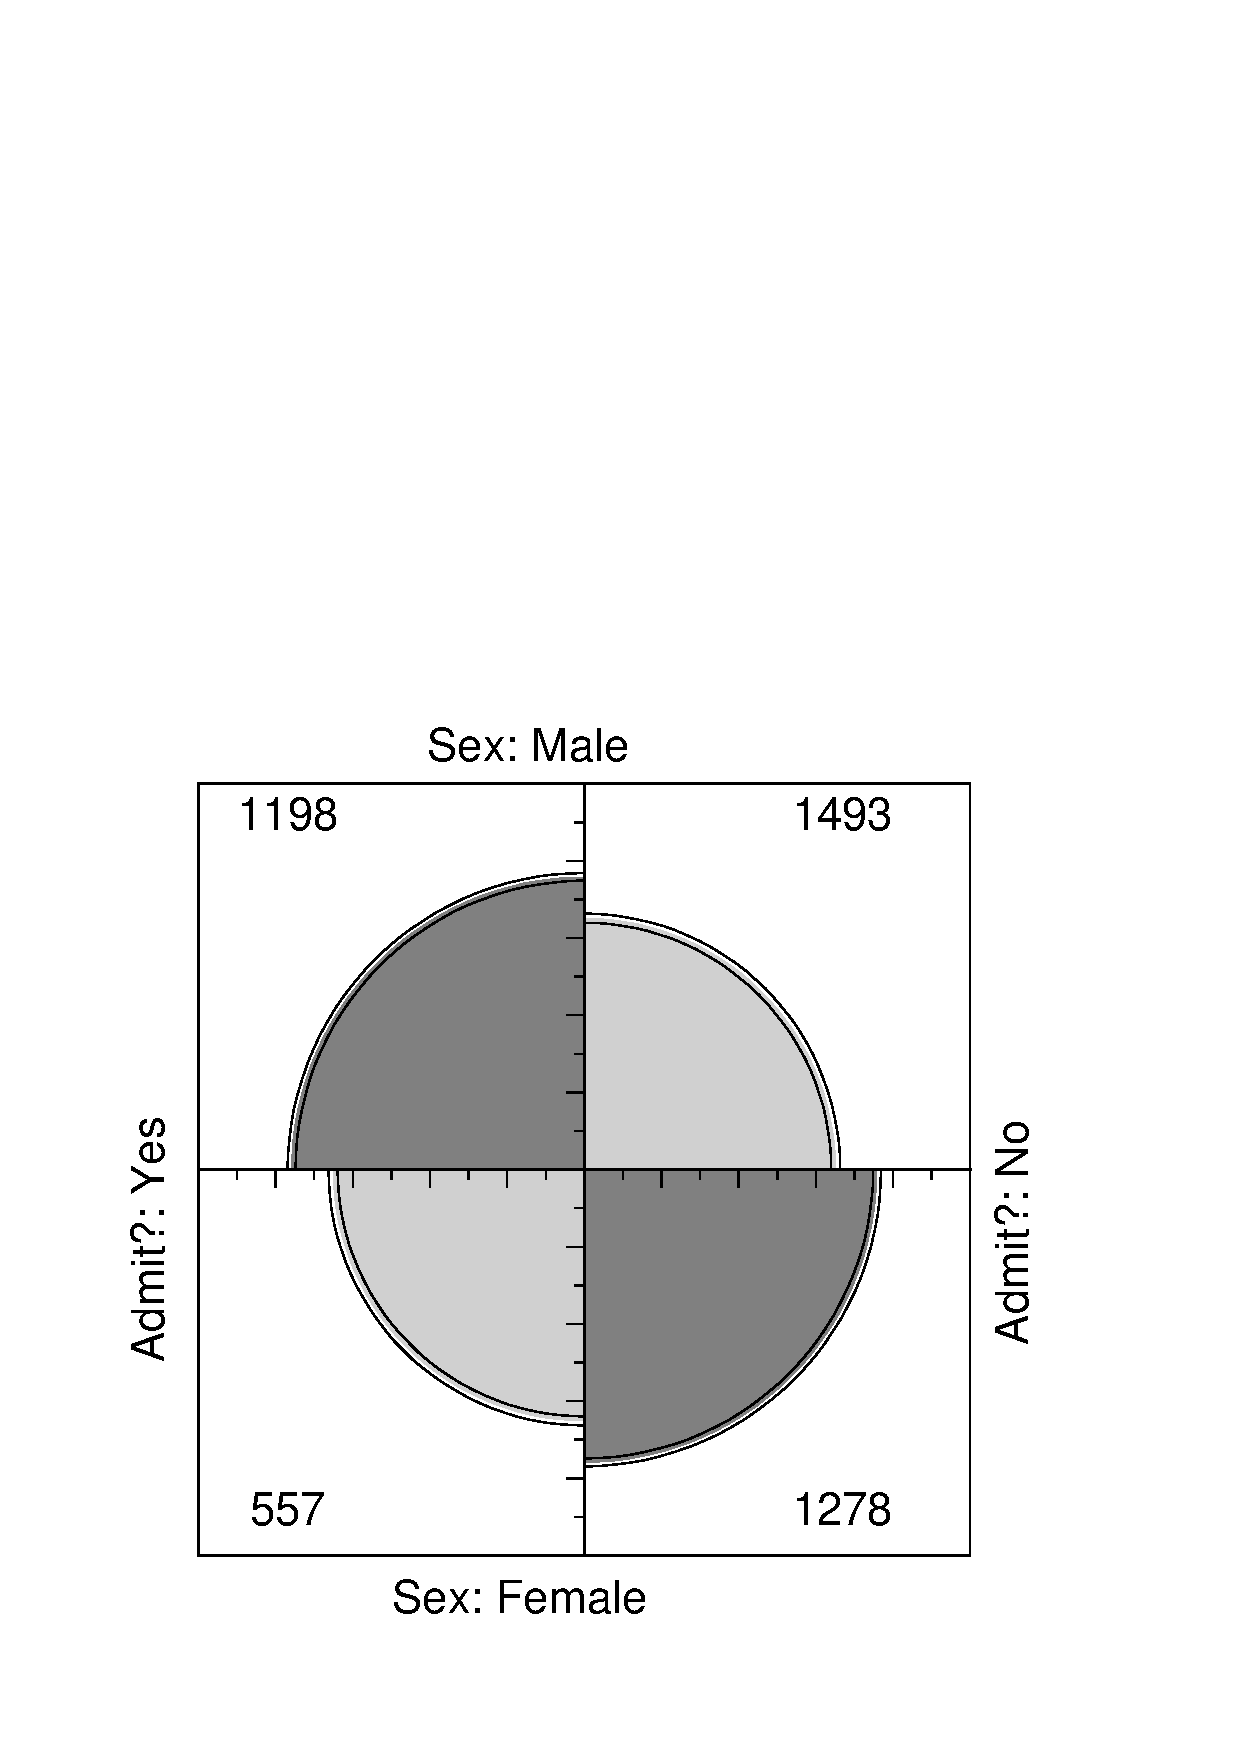
\includegraphics[width=1\linewidth,clip]{ch3/fig/fourfold13}
 \end{minipage}%
 \hfill
 \begin{minipage}[c]{.33\linewidth}
  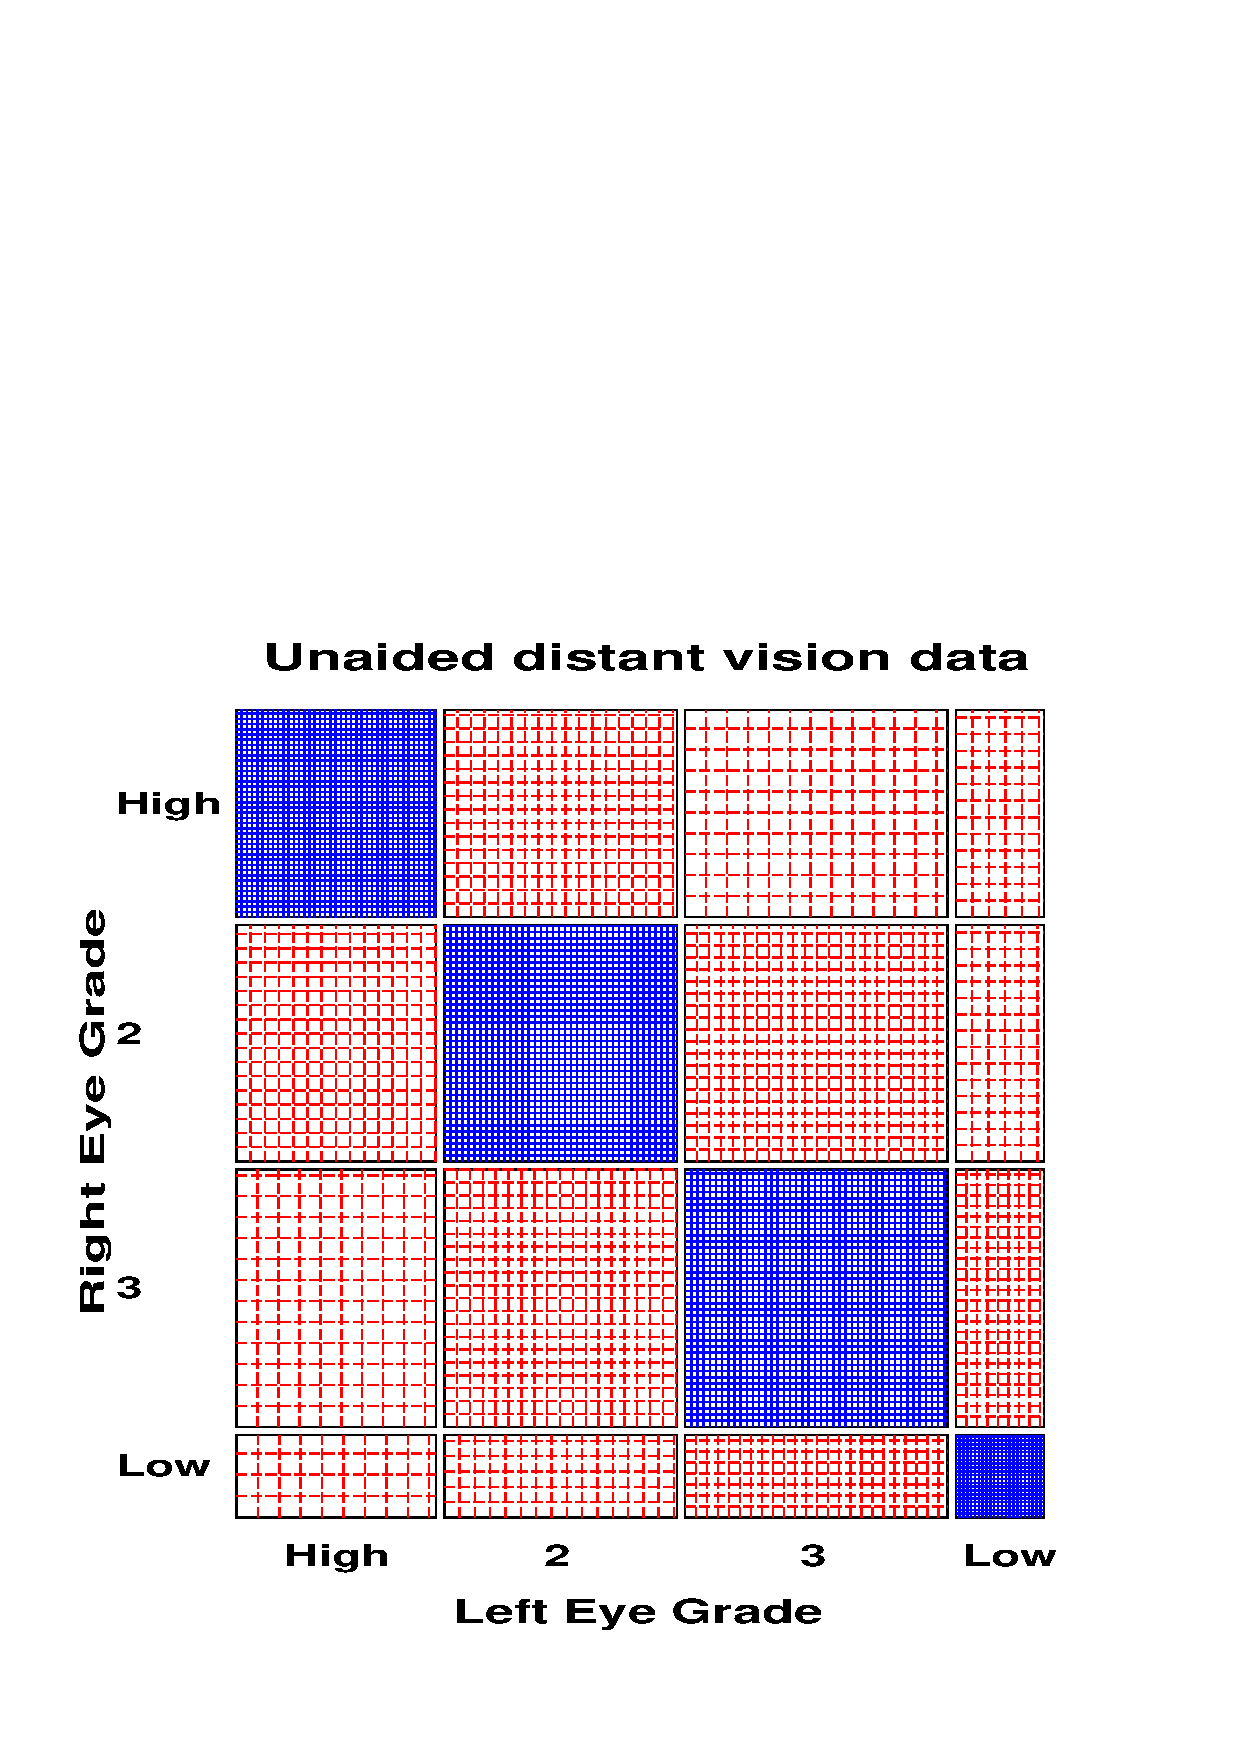
\includegraphics[width=1\linewidth,clip]{ch3/fig/sieve2}
 \end{minipage}
 \hfill
 \begin{minipage}[c]{.33\linewidth}
  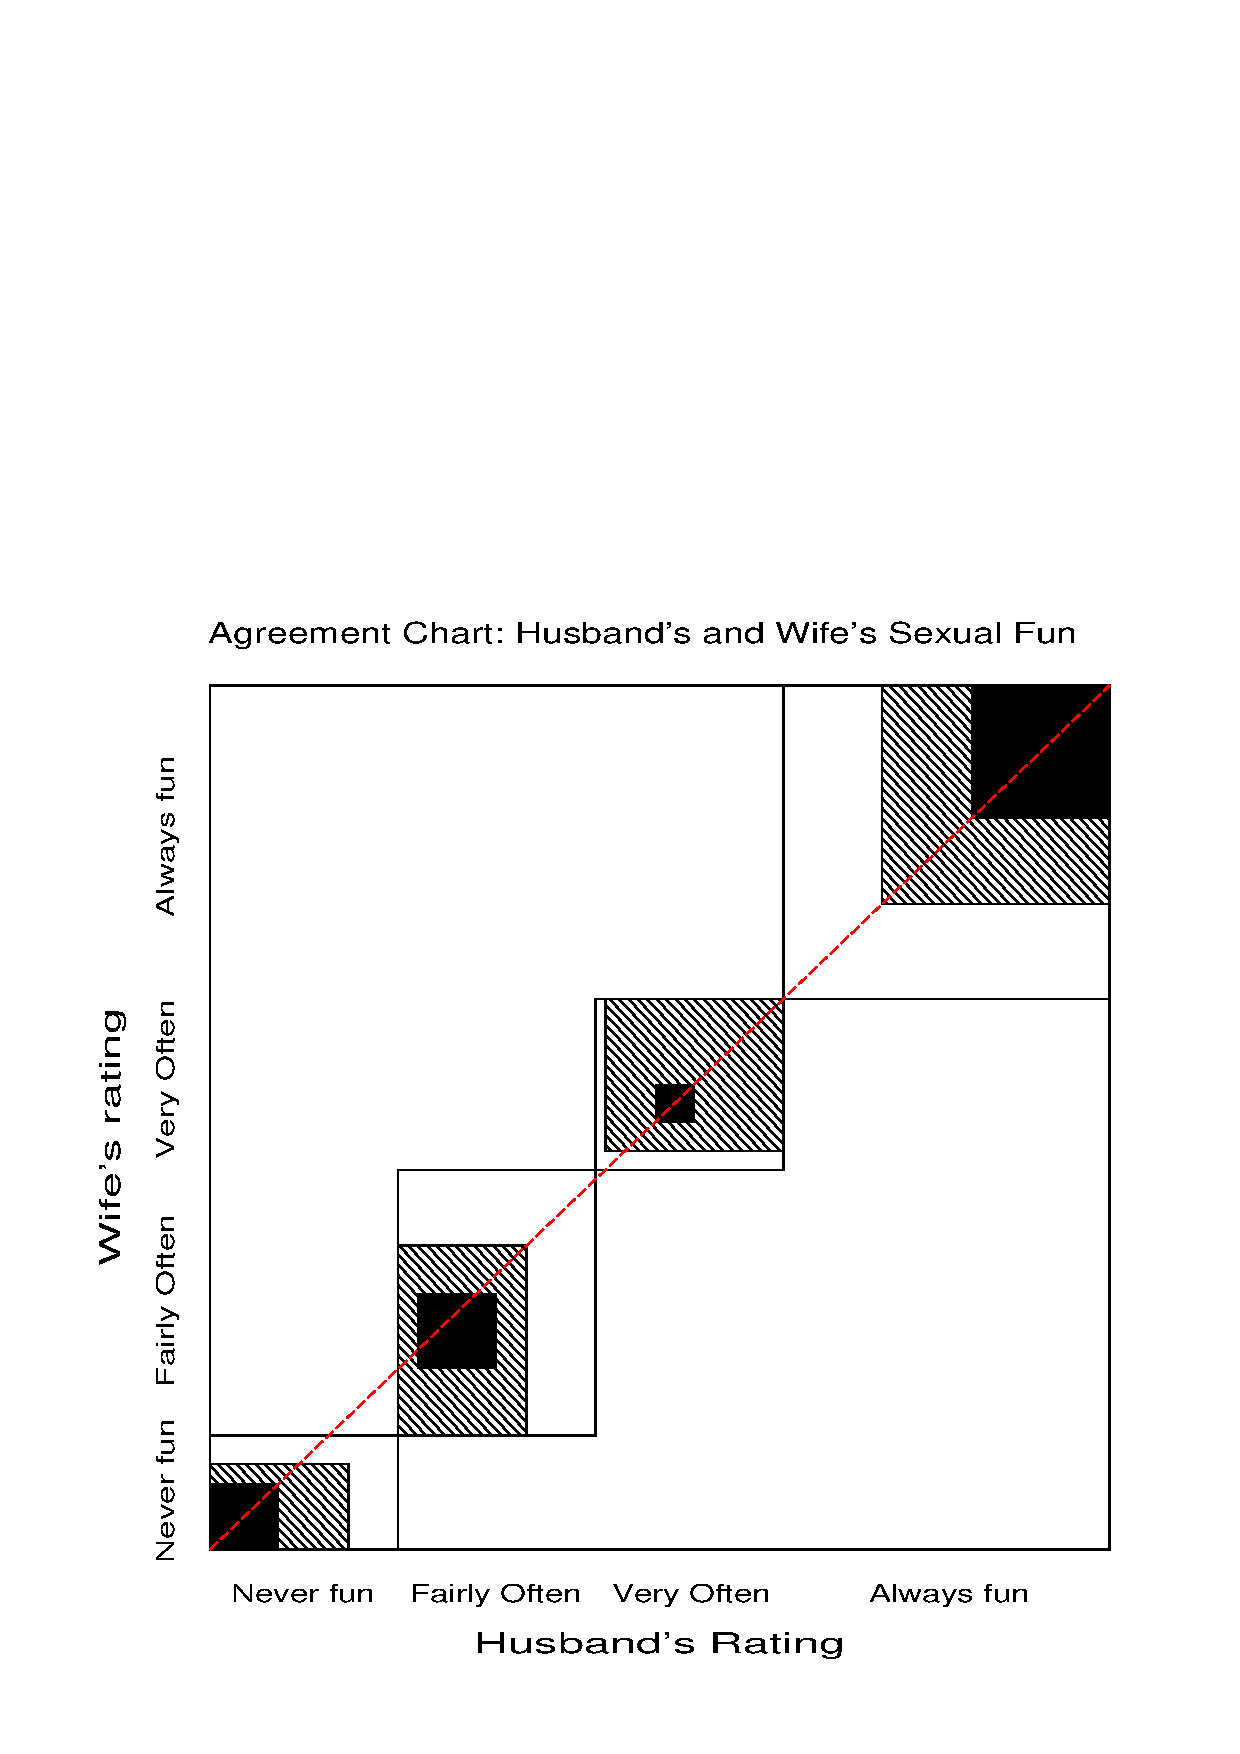
\includegraphics[width=1\linewidth,clip]{ch3/fig/agree12}
 \end{minipage}
\end{center}

   %% visual contents images

\chapterprelude{
Discrete data often follow various theoretical probability models.
Graphic displays are used to visualize goodness of fit,
to diagnose an appropriate model, and determine the impact of
individual observations on estimated parameters.
}
% \minitoc
% \clearpage

\epigraph{Not everything that counts can be counted, and not everything that
can be counted counts.}
{Albert Einstein}

Discrete frequency distributions often involve counts of occurrences of events,
such as accident fatalities, incidents of terrorism or suicide,
words in passages of text, or blood cells with some characteristic.
Often interest is focused on how closely such data follow a particular probability distribution,
such as the binomial, Poisson, or geometric distribution, which
provide the basis for generating mechanisms that might give rise to the
data.
Understanding and visualizing
such distributions
in the simplest case of an unstructured sample provides a building block for generalized
linear models (\chref{ch:glm}) where they serve as one component.  The also provide the basis for
a variety of recent extensions of regression models for count data (\chref{ch:glm}),
allowing excess counts of zeros (zero-inflated models), left- or right-
truncation often encountered in statistical practice.

\TODO{DM: Fix chapter ref if ch.09 gets split}

This chapter describes the well-known discrete
frequency distributions: the binomial, Poisson, negative binomial,
geometric, and logarithmic series distributions in the simplest case of an unstructured sample.
The chapter begins with simple graphical displays (line graphs and bar charts) to view
the distributions of empirical data and theoretical frequencies from a specified
discrete distribution.

It then describes methods for fitting data to a distribution of a given form
and simple, effective
graphical methods than can be used to visualize goodness of fit,
to diagnose an appropriate model (e.g., does a given data set follow the
Poisson or negative binomial?) and determine the impact of
individual observations on estimated parameters.

\section{Introduction to discrete distributions}\label{sec:discrete-intro}
Discrete data analysis is concerned with the study of the tabulation of one or
more types of events, often categorized into mutually exclusive and exhaustive
categories.  \term{Binary events} having two outcome categories include
the toss of a coin (head/tails), sex of a child (male/female), survival of
a patient following surgery (lived/died), and so forth.  \term{Polytomous events}
have more outcome categories, which may be \emph{ordered}
(rating of impairment: low/medium/high, by a physician)
and possibly numerically-valued
(number of dots (pips), 1--6 on the toss of a die)
or \emph{unordered} (political party supported: Liberal, Conservative, Greens, Socialist).

In this chapter, we focus largely on one-way frequency tables for a single
numerically-valued variable.
Probability models for such data provide the opportunity to describe or explain
the \emph{structure} in such data, in that they entail some data generating
mechanism and provide the basis for testing scientific hypotheses, prediction of
future results.  If a given probability model does not fit the data, this can often
be a further opportunity to extend understanding of the data or the underlying
substantive theory or both.

The remainder of this section gives a few substantive examples of situations where the
well-known discrete frequency distributions (binomial, Poisson, negative binomial,
geometric, and logarithmic series) might reasonably apply, at least approximately.
The mathematical characteristics and properties of these theoretical
distributions are postponed to \secref{sec:discrete-distrib}.

In many cases, the data at hand pertain to two types of variables in a one-way
frequency table. There is a basic outcome variable, $k$, taking integer values,
$k = 0, 1, \dots$, and called a \term{count}.  For each value of $k$, we also have
a \term{frequency}, $n_k$ that the count $k$ was observed in some sample.
For example, in the study of children in families, the count variable
$k$ could be the total number of children or the number of male children;
the frequency variable, $n_k$, would then give the number of families with that
basic count $k$.

\subsection{Binomial data}\label{sec:binom-data}
Binomial type data arise as the discrete distribution of the number of
``success'' events in $n$ independent binary trials, each of which
yields a success (yes/no, head/tail, lives/dies, male/female) with a constant probability $p$.

Sometimes, as in \exref{ex:arbuthnot1}
below, the available data record only the number of successes
in $n$ trials, with separate such observations recorded over
time or space.  More commonly, as in \exref{ex:saxony1}
and \exref{ex:dice},
we have available data on the frequency $n_k$
of $k = 0, 1, 2, \dots n$ successes in the $n$ trials.


\begin{Example}[arbuthnot1]{Arbuthnot data}
Sex ratios--- births of male to female children have long been of interest
in population studies and demography. Indeed, in 1710, John Arbuthnot \citep{Arbuthnot:1710}
used data on the ratios of male to female christenings in London from 1629--1710 to carry out the first known significance test.
The data for these 82 years showed that in \emph{every} year there were more boys than girls.
He calculated that the under the assumption
that male and female births were equally likely, the probability of 82 years of
more males than females was vanishingly small,
 ($\Pr \approx 4.14 \times 10^{-25}$).
He used this to argue that a nearly constant birth ratio $> 1$ (or $\Pr(\mathrm{Male}) > 0.5$)
could be interpreted to show the guiding hand of a divine being.

Arbuthnot's data, along with some other related variables
are available in \data{Arbuthnot} in the \Rpackage{HistData}.
For now, we simply display a plot of the probability of a male birth over time.
The plot in \figref{fig:arbuthnot1} shows the proportion of males over years,
with horizontal lines at $\Pr(\mathrm{Male}) = 0.5$ and the mean,
$\Pr(\mathrm{Male}) = 0.517$.  Also shown is a (loess) smoothed curve, which suggests
that any deviation from a constant sex ratio is relatively small.
\begin{knitrout}
\definecolor{shadecolor}{rgb}{1, 0.961, 0.933}\color{fgcolor}\begin{kframe}
\begin{alltt}
\hlstd{> }\hlkwd{data}\hlstd{(Arbuthnot,} \hlkwc{package} \hlstd{=} \hlstr{"HistData"}\hlstd{)}
\hlstd{> }\hlkwd{with}\hlstd{(Arbuthnot, \{}
\hlstd{+ }  \hlstd{prob} \hlkwb{=} \hlstd{Males} \hlopt{/} \hlstd{(Males} \hlopt{+} \hlstd{Females)}
\hlstd{+ }  \hlkwd{plot}\hlstd{(}\hlkwc{x} \hlstd{= Year,} \hlkwc{y} \hlstd{= prob,} \hlkwc{type} \hlstd{=} \hlstr{"b"}\hlstd{,}
\hlstd{+ }       \hlkwc{ylim} \hlstd{=} \hlkwd{c}\hlstd{(}\hlnum{0.5}\hlstd{,} \hlnum{0.54}\hlstd{),} \hlkwc{ylab} \hlstd{=} \hlstr{"Pr (Male)"}\hlstd{)}
\hlstd{+ }  \hlkwd{abline}\hlstd{(}\hlkwc{h} \hlstd{=} \hlnum{0.5}\hlstd{,} \hlkwc{col} \hlstd{=} \hlstr{"red"}\hlstd{,} \hlkwc{lwd} \hlstd{=} \hlnum{2}\hlstd{)}
\hlstd{+ }  \hlkwd{abline}\hlstd{(}\hlkwc{h} \hlstd{=} \hlkwd{mean}\hlstd{(prob),} \hlkwc{col} \hlstd{=} \hlstr{"blue"}\hlstd{)}
\hlstd{+ }  \hlkwd{text}\hlstd{(}\hlkwc{x} \hlstd{=} \hlnum{1640}\hlstd{,} \hlkwc{y} \hlstd{=} \hlnum{0.5}\hlstd{,} \hlkwd{expression}\hlstd{(H[}\hlnum{0}\hlstd{]}\hlopt{:} \hlstr{"Pr(Male)=0.5"}\hlstd{),} \hlkwc{pos} \hlstd{=} \hlnum{3}\hlstd{,} \hlkwc{col} \hlstd{=} \hlstr{"red"}\hlstd{)}
\hlstd{+ }  \hlstd{Arb.smooth} \hlkwb{<-} \hlkwd{loess.smooth}\hlstd{(Year, prob)}
\hlstd{+ }  \hlkwd{lines}\hlstd{(Arb.smooth,} \hlkwc{col} \hlstd{=} \hlstr{"blue"}\hlstd{,} \hlkwc{lwd} \hlstd{=} \hlnum{2}\hlstd{)}
\hlstd{+ }  \hlstd{\})}
\end{alltt}
\end{kframe}\begin{figure}[!htbp]

\centerline{\includegraphics[width=.75\textwidth]{ch03/fig/arbuthnot1-1} }

\caption[Arbuthnot's data on male/female sex ratios]{Arbuthnot's data on male/female sex ratios in London, 1629--1710, together with a (loess) smoothed curve over time and the mean Pr(Male)\label{fig:arbuthnot1}}
\end{figure}


\end{knitrout}

\TODO{DM: use slightly simpler alternative? :}

\begin{knitrout}
\definecolor{shadecolor}{rgb}{1, 0.961, 0.933}\color{fgcolor}\begin{kframe}
\begin{alltt}
\hlstd{> }\hlstd{prob} \hlkwb{<-} \hlkwd{with}\hlstd{(Arbuthnot, Males} \hlopt{/} \hlstd{(Males} \hlopt{+} \hlstd{Females))}
\hlstd{> }\hlkwd{scatter.smooth}\hlstd{(}\hlkwc{x} \hlstd{= Arbuthnot}\hlopt{$}\hlstd{Year,} \hlkwc{y} \hlstd{= prob,} \hlkwc{type} \hlstd{=} \hlstr{"b"}\hlstd{,}
\hlstd{+ }               \hlkwc{lpars} \hlstd{=} \hlkwd{list}\hlstd{(}\hlkwc{col} \hlstd{=} \hlstr{"blue"}\hlstd{,} \hlkwc{lwd} \hlstd{=} \hlnum{2}\hlstd{),}
\hlstd{+ }               \hlkwc{xlab} \hlstd{=} \hlstr{"Year"}\hlstd{,} \hlkwc{ylab} \hlstd{=} \hlstr{"Pr(Male)"}\hlstd{,} \hlkwc{ylim} \hlstd{=} \hlkwd{c}\hlstd{(}\hlnum{0.5}\hlstd{,} \hlnum{0.54}\hlstd{))}
\hlstd{> }\hlkwd{abline}\hlstd{(}\hlkwc{h} \hlstd{=} \hlnum{0.5}\hlstd{,} \hlkwc{col} \hlstd{=} \hlstr{"red"}\hlstd{,} \hlkwc{lwd} \hlstd{=} \hlnum{2}\hlstd{)}
\hlstd{> }\hlkwd{abline}\hlstd{(}\hlkwc{h} \hlstd{=} \hlkwd{mean}\hlstd{(prob),} \hlkwc{col} \hlstd{=} \hlstr{"blue"}\hlstd{)}
\hlstd{> }\hlkwd{text}\hlstd{(}\hlkwc{x} \hlstd{=} \hlnum{1640}\hlstd{,} \hlkwc{y} \hlstd{=} \hlnum{0.5}\hlstd{,} \hlkwd{expression}\hlstd{(H[}\hlnum{0}\hlstd{]}\hlopt{:} \hlstr{"Pr(Male)=0.5"}\hlstd{),} \hlkwc{pos} \hlstd{=} \hlnum{3}\hlstd{,} \hlkwc{col} \hlstd{=} \hlstr{"red"}\hlstd{)}
\end{alltt}
\end{kframe}\begin{figure}[!htbp]

\centerline{\includegraphics[width=.75\textwidth]{ch03/fig/arbuthnot12-1} }

\caption[Arbuthnot's data on male/female sex ratios]{Arbuthnot's data on male/female sex ratios in London, 1629--1710, together with a (loess) smoothed curve over time and the mean Pr(Male)\label{fig:arbuthnot12}}
\end{figure}


\end{knitrout}

We return to this data in a later chapter where we ask whether the variation around
the mean can be explained by any other considerations, or should just be considered
random variation (see \labref{lab:7.1})
\end{Example}

\begin{Example}[saxony1]{Families in Saxony}
A related example of sex ratio data that ought to follow a binomial distribution
comes from a classic study by A. Geissler \citeyearpar{Geissler:1889}.
Geissler listed the data on the distributions of boys and girls in families
in Saxony for the period 1876--1885. In total, over four million births were
recorded, and the sex distribution in the family was available because the parents had to state the sex of all their children on
the birth certificate.%

The complete data, classified by number of boys and number of girls
(each 0--12) appear in \citet[Table 1]{Edwards:1958}.%
\footnote{
\citet{Edwards:1958} notes that over these 10 years, many parents
will have had several children, and their family composition
is therefore recorded more than once.  However, in families with a given
number of children, each family can appear only once.
}
\citet[Table 6.2]{Lindsey:95} selected only the 6115 families with
12 children, and listed the frequencies by number of males.  The
data are shown in table form in \tabref{tab:saxtab} in the standard form
of a complete discrete distribution.  The basic outcome variable,
$k = 0, 1, \dots, 12$, is the number of male children in a family
and the frequency variable, $n_k$ is the number of families with that
number of boys.

% latex table generated in R 3.0.1 by xtable 1.7-1 package
% Tue Nov 26 14:56:02 2013
\begin{table}[t]
\caption{Number of male children in 6115 Saxony families of size 12} \label{tab:saxtab}
\centering
\begin{tabular}{l|rrrrrrrrrrrrr}
  \hline
Males ($k$) & 0 & 1 & 2 & 3 & 4 & 5 & 6 & 7 & 8 & 9 & 10 & 11 & 12 \\ 
  \hline
Families ($n_k$) & 3 & 24 & 104 & 286 & 670 & 1,033 & 1,343 & 1,112 & 829 & 478 & 181 & 45 & 7  \\ 
   \hline
\end{tabular}
\end{table}
 


\figref{fig:saxony-barplot} shows a bar plot of the frequencies in \tabref{tab:saxtab}.
It can be seen that the distribution is quite symmetric.  The questions of interest
here are:
(a) how close does the data follow a binomial distribution, with a constant
$\Pr(\mathrm{Male}) = p$?
(b) is there evidence to reject the hypothesis that $ p = 0.5$?

\begin{knitrout}
\definecolor{shadecolor}{rgb}{1, 0.961, 0.933}\color{fgcolor}\begin{kframe}
\begin{alltt}
\hlstd{> }\hlkwd{data}\hlstd{(Saxony,} \hlkwc{package} \hlstd{=} \hlstr{"vcd"}\hlstd{)}
\hlstd{> }\hlkwd{barplot}\hlstd{(Saxony,} \hlkwc{xlab} \hlstd{=} \hlstr{"Number of males"}\hlstd{,} \hlkwc{ylab} \hlstd{=} \hlstr{"Number of families"}\hlstd{,}
\hlstd{+ }        \hlkwc{col} \hlstd{=} \hlstr{"lightblue"}\hlstd{,} \hlkwc{cex.lab} \hlstd{=} \hlnum{1.5}\hlstd{)}
\end{alltt}
\end{kframe}\begin{figure}[!htbp]

\centerline{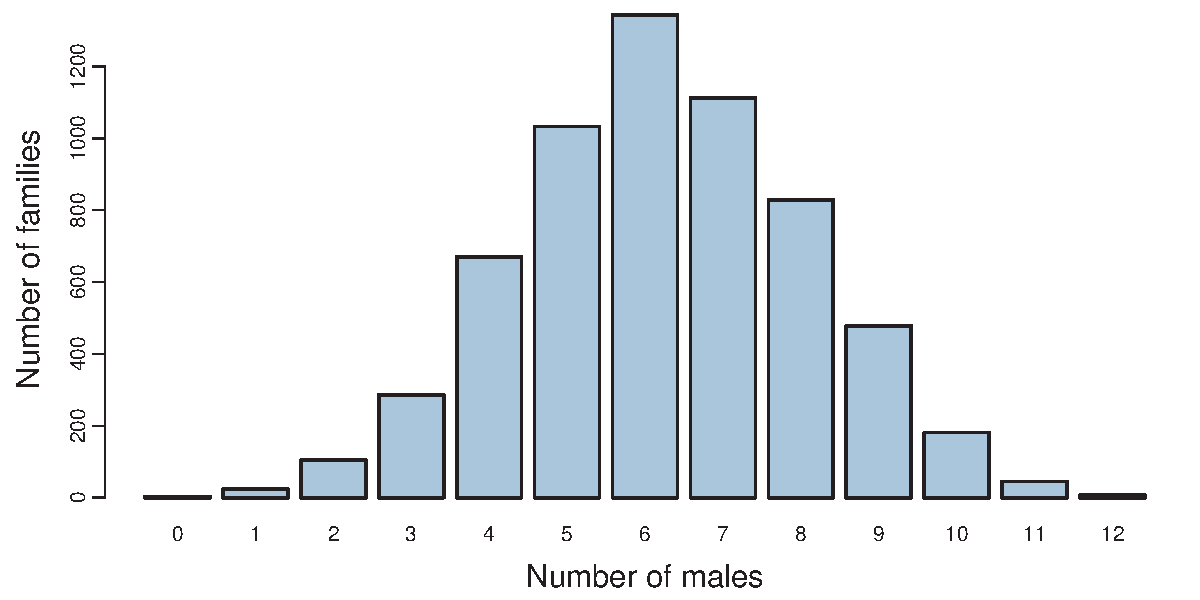
\includegraphics[width=.75\textwidth]{ch03/fig/saxony-barplot-1} }

\caption[Males in Saxony families of size 12]{Males in Saxony families of size 12\label{fig:saxony-barplot}}
\end{figure}


\end{knitrout}
\end{Example}

\begin{Example}[dice]{Weldon's dice}
Common examples of binomial distributions involve tossing coins
or dice, where some event outcome is considered a ``success''
and the number of successes ($k$) are tabulated
in a long series of trials to give the frequency ($n_k$)
of each basic count, $k$.

Perhaps the most industrious dice-tosser of all times,
W. F. Raphael Weldon, an English evolutionary biologist
and joint founding editor of \emph{Biometrika} (with Francis Galton and Karl Pearson)
tallied the results of throwing 12 dice 26,306 times.
For his purposes, he considered the outcome of 5 or 6 pips showing on each die
to be a success, and all other outcomes as failures.

Weldon reported his results in a letter to Francis Galton dated
February 2, 1894, in order
``to judge whether the differences between a series of group frequencies
and a theoretical law \dots were more than might be attributed
to the chance fluctuations of random sampling''
\citep{KempKemp:91}.
In his seminal paper,
\citet{Pearson:00} used Weldon's data to illustrate the \chisq{} goodness-of-fit test, as did
\citet[Table 5.1, p. 121]{KendallStuart:63}.

These data are
shown here as
\tabref{tab:dicetab},
in terms of the number of occurrences of a 5 or
6 in the throw of 12 dice.
If the dice were all identical and perfectly fair (balanced), one would
expect that $p = \Pr\{5 \textrm{ or } 6\} = \frac13$
and the distribution of the number of 5 or 6 would be binomial.

A peculiar feature of these data
as presented by Kendall and Stuart (not uncommon in discrete distributions)
is that the frequencies of 10--12 successes
are lumped together.%
\footnote{
The unlumped entries are, for (number of 5s or 6s: frequency) ---
(10: 14); (11: 4), (12:0),
given by \citet{Labby:2009}.
In this remarkable paper, Labby describes a mechanical device he constructed to
repeat Weldon's experiment physically and automate the counting of outcomes.
He created electronics to roll 12 dice in a physical box, and hooked that
up to a webcam to capture an image of each toss and used image processing
software to record the counts.
}
This grouping must be taken into account in fitting
the distribution.  This dataset is available as \data{WeldonDice} in the
\Rpackage{vcd}.  The distribution is plotted in \figref{fig:dice}.

% latex table generated in R 3.0.1 by xtable 1.7-1 package
% Thu Nov 28 15:27:53 2013
\begin{table}[tb]
\centering
\caption{Frequencies of 5s or 6s in throws of 12 dice} \label{tab:dicetab}
\begin{tabular}{l|rrrrrrrrrrr}
   \hline
\# 5s or 6s ($k$) & 0 & 1 & 2 & 3 & 4 & 5 & 6 & 7 & 8 & 9 & 10+ \\ 
Frequency ($n_k$) &   185 &  1,149 &  3,265 &  5,475 &  6,114 &  5,194 &  3,067 &  1,331 &   403 &   105 &    18  \\ 
   \hline
\end{tabular}
\end{table}



%%% one figure
%\begin{figure}[htb]
%%  \SASfig{dice.eps}{scale=.65}{dice}{Weldon's dice data}
%  \centering
%  \includegraphics[scale=.65]{dice.eps}
%  \caption{Weldon's dice data}%
%  \label{fig:dice}
%\end{figure}

\begin{knitrout}
\definecolor{shadecolor}{rgb}{1, 0.961, 0.933}\color{fgcolor}\begin{kframe}
\begin{alltt}
\hlstd{> }\hlkwd{data}\hlstd{(WeldonDice,} \hlkwc{package} \hlstd{=} \hlstr{"vcd"}\hlstd{)}
\hlstd{> }\hlkwd{dimnames}\hlstd{(WeldonDice)}\hlopt{$}\hlstd{n56[}\hlnum{11}\hlstd{]} \hlkwb{<-} \hlstr{"10+"}
\hlstd{> }\hlkwd{barplot}\hlstd{(WeldonDice,} \hlkwc{xlab} \hlstd{=} \hlstr{"Number of 5s and 6s"}\hlstd{,} \hlkwc{ylab} \hlstd{=} \hlstr{"Frequency"}\hlstd{,}
\hlstd{+ }        \hlkwc{col} \hlstd{=} \hlstr{"lightblue"}\hlstd{,} \hlkwc{cex.lab} \hlstd{=} \hlnum{1.5}\hlstd{)}
\end{alltt}
\end{kframe}\begin{figure}[!htbp]

\centerline{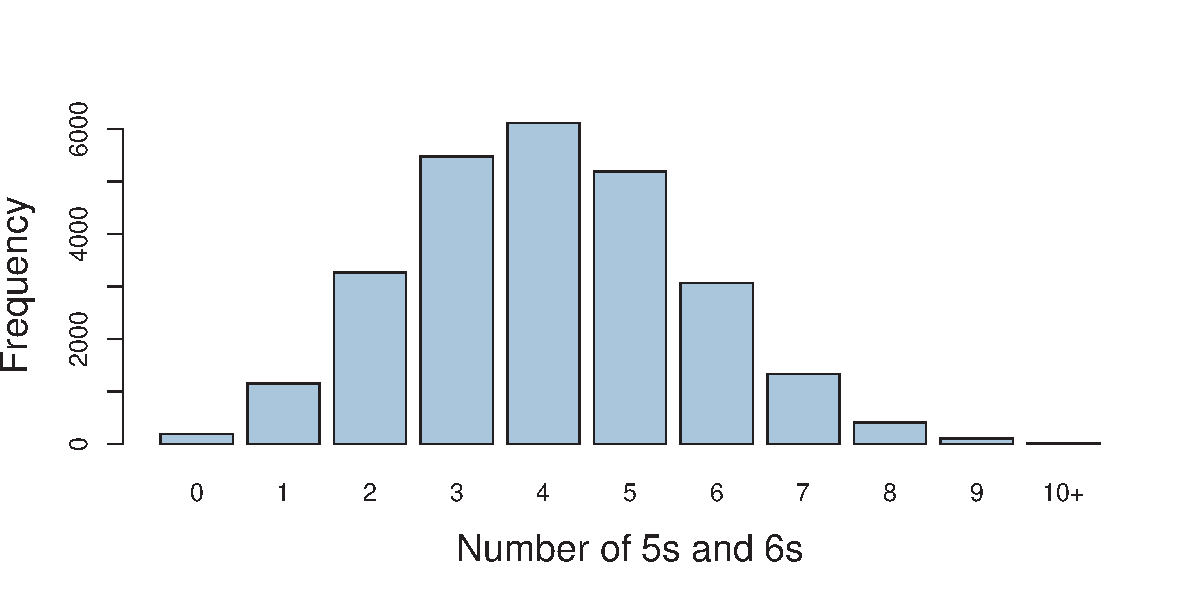
\includegraphics[width=.75\textwidth]{ch03/fig/dice-1} }

\caption[Weldon's dice data]{Weldon's dice data\label{fig:dice}}
\end{figure}


\end{knitrout}
\end{Example}

\subsection{Poisson data}\label{sec:pois-data}

Data of Poisson type arise when we observe the counts of events $k$ within a
fixed interval of time or space (length, area, volume) and tabulate their
frequencies, $n_k$.  For example, we may observe the number of radioactive
particles emitted by a source per second or number of births per hour,
or the number of tiger or whale sightings within some geographical regions.

In contrast to binomial data, where the counts are bounded below and above,
in Poisson data the counts $k$ are bounded below at 0, but can take integer
values with no fixed upper limit.
One defining characteristic for the Poisson distribution is for rare
events, which occur independently with a small and constant
probability, $p$, in small intervals, and we count the number of such occurrences.

Several examples of data of this general type are given below.

\begin{Example}[horsekick1]{Death by horse kick}
One of the oldest and best known examples of a Poisson distribution
is the data from
\citet{Bortkiewicz:98} on deaths of soldiers in the Prussian
army from kicks by horses and mules, shown in \tabref{tab:horsetab}.
Ladislaus von Bortkiewicz, an economist and statistician,
tabulated the number of soldiers in each of
14 army corps in the 20 years from 1875-1894
who died after being kicked by a horse
\citep[p. 18]{AndrewsHerzberg:85}.
\tabref{tab:horsetab} shows the data used by
\citet{Fisher:25} for 10 of these
army corps, summed over 20 years, giving 200
`corps-year' observations.  In 109 corps-years,
no deaths occurred; 65 corps-years had one death, etc.

The data set is available as \data{HorseKicks} in the \Rpackage{vcd}.
The distribution is plotted in \figref{fig:horsekicks}.
% latex table generated in R 3.0.1 by xtable 1.7-1 package
% Fri Nov 29 08:56:45 2013
\begin{table}[tb]
\centering
\caption{von Bortkiewicz's data on deaths by horse kicks} \label{tab:horsetab}
\begin{tabular}{l|rrrrr|r}
   \hline
Number of deaths ($k$) & 0 & 1 & 2 & 3 & 4 & Sum \\ 
  Frequency ($n_k$) & 109 &  65 &  22 &   3 &   1 & 200 \\ 
   \hline
\end{tabular}
\end{table}


\begin{knitrout}
\definecolor{shadecolor}{rgb}{1, 0.961, 0.933}\color{fgcolor}\begin{kframe}
\begin{alltt}
\hlstd{> }\hlkwd{data}\hlstd{(HorseKicks,} \hlkwc{package} \hlstd{=} \hlstr{"vcd"}\hlstd{)}
\hlstd{> }\hlkwd{barplot}\hlstd{(HorseKicks,} \hlkwc{xlab} \hlstd{=} \hlstr{"Number of deaths"}\hlstd{,} \hlkwc{ylab} \hlstd{=} \hlstr{"Frequency"}\hlstd{,}
\hlstd{+ }        \hlkwc{col} \hlstd{=} \hlstr{"lightblue"}\hlstd{,} \hlkwc{cex.lab} \hlstd{=} \hlnum{1.5}\hlstd{)}
\end{alltt}
\end{kframe}\begin{figure}[!htbp]

\centerline{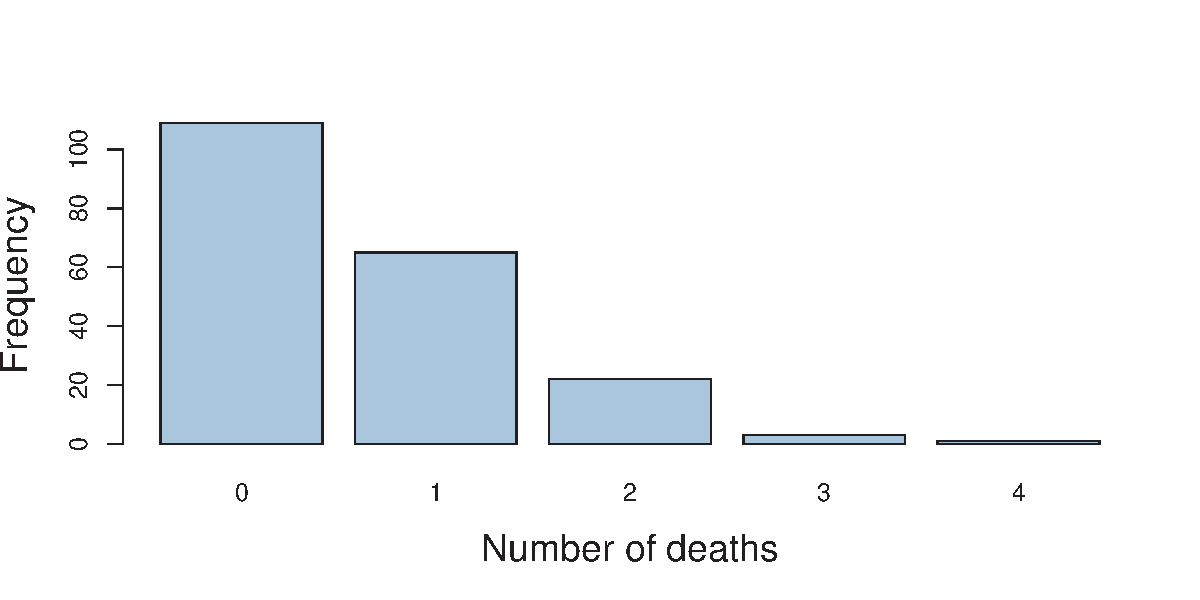
\includegraphics[width=.75\textwidth]{ch03/fig/horsekicks-1} }

\caption[HorseKicks data]{HorseKicks data\label{fig:horsekicks}}
\end{figure}


\end{knitrout}
\end{Example}

\begin{Example}[madison1]{Federalist papers}
In 1787--1788, Alexander Hamilton, John Jay, and James Madison
wrote a series of newspaper essays to persuade the voters of
New York State to ratify the U.S. Constitution.
The essays were titled \emph{The Federalist Papers}
and all were signed with the pseudonym ``Publius.''  Of the 77 papers published,
the author(s) of 65 are known, but \emph{both}
Hamilton and Madison later claimed sole authorship of the remaining 12.
\citet{MostellerWallace:63,MostellerWallace:84}
investigated the use of statistical methods to identify authors of
disputed works based on the frequency distributions of certain key
function words, and concluded that Madison had indeed authored the
12 disputed papers.%
\footnote{
It should be noted that this is a landmark work in the development and
application of statistical methods to the analysis of texts and
cases of disputed authorship. In addition to
\emph{may}, they considered many such marker words,
such as \emph{any}, \emph{by}, \emph{from}, \emph{upon}, and so forth.
Among these, the word \emph{upon} was the best discriminator between
the works known by Hamilton (3 per 1000 words) and Madison (1/6 per 1000 words).
In this work, they pioneered the use of Bayesian discriminant analysis,
and the use of cross-validation to assess the stability of estimates
and their conclusions.
}

\tabref{tab:fedtab} shows the distribution of the occurrence of one of
these ``marker'' words,
the
word \emph{may} in 262 blocks of text (each about 200 words long)
from issues of the \emph{Federalist Papers} and other essays known
to be written by James Madison.  Read the table as follows:
in 156 blocks, the word \emph{may}
did not occur; it occurred once in 63 blocks, etc.  The distribution
is plotted in \figref{fig:federalist}.

% latex table generated in R 3.0.1 by xtable 1.7-1 package
% Fri Nov 29 14:25:47 2013
\begin{table}[htb]
\centering
\caption{Number of occurrences of the word \emph{may} in texts written by James Madison\label{tab:fedtab}} 
\begin{tabular}{l|rrrrrrr|r}
   \hline
Occurrences of \emph{may} ($k$) & 0 & 1 & 2 & 3 & 4 & 5 & 6 & Sum \\ 
  Blocks of text ($n_k$)       & 156 &  63 &  29 &   8 &   4 &   1 &   1 & 262 \\ 
   \hline
\end{tabular}
\end{table}

\begin{knitrout}
\definecolor{shadecolor}{rgb}{1, 0.961, 0.933}\color{fgcolor}\begin{kframe}
\begin{alltt}
\hlstd{> }\hlkwd{data}\hlstd{(Federalist,} \hlkwc{package} \hlstd{=} \hlstr{"vcd"}\hlstd{)}
\hlstd{> }\hlkwd{barplot}\hlstd{(Federalist,}
\hlstd{+ }        \hlkwc{xlab} \hlstd{=} \hlstr{"Occurrences of 'may'"}\hlstd{,} \hlkwc{ylab} \hlstd{=} \hlstr{"Number of blocks of text"}\hlstd{,}
\hlstd{+ }        \hlkwc{col} \hlstd{=} \hlstr{"lightgreen"}\hlstd{,} \hlkwc{cex.lab} \hlstd{=} \hlnum{1.5}\hlstd{)}
\end{alltt}
\end{kframe}\begin{figure}[!htbp]

\centerline{\includegraphics[width=.75\textwidth]{ch03/fig/federalist-1} }

\caption[Mosteller and Wallace Federalist data]{Mosteller and Wallace Federalist data\label{fig:federalist}}
\end{figure}


\end{knitrout}
\end{Example}

\begin{Example}[cyclists1]{London cycling deaths}

\citet{AberdeinSpiegelhalter:2013} observed that from November 5--13, 2013,
six people were killed while cycling in London.  How unusual is this
number of deaths in less than a two-week period?
Was this a freak occurrence, or should Londoners petition for
cycling lanes and greater road safety?
To answer these question, they obtained data from the
UK Department of Transport \emph{Road Safety Data} from 2005--2012
and selected all accident fatalities of cyclists within the
city of London.

It seems reasonable to assume that, in any short period of time, deaths of
people riding bicycles are independent events.  If, in addition,
the probability of such events is constant over this time span,
the Poisson distribution should describe the distribution of
$0, 1, 2, 3, \dots$ deaths. Then, an answer to the main question can be
given in terms of the probability of six (or more) deaths in
a comparable period of time.

Their data, comprising 208 counts of deaths in the fortnightly periods
from January 2005 to December 2012 are contained in the \Dset
\data{CyclingDeaths} in \pkg{vcdExtra}.  To work with the
distribution, we first convert this to a one-way table.

\begin{knitrout}
\definecolor{shadecolor}{rgb}{1, 0.961, 0.933}\color{fgcolor}\begin{kframe}
\begin{alltt}
\hlstd{> }\hlkwd{data}\hlstd{(}\hlstr{"CyclingDeaths"}\hlstd{,} \hlkwc{package} \hlstd{=} \hlstr{"vcdExtra"}\hlstd{)}
\hlstd{> }\hlstd{CyclingDeaths.tab} \hlkwb{<-} \hlkwd{table}\hlstd{(CyclingDeaths}\hlopt{$}\hlstd{deaths)}
\hlstd{> }\hlstd{CyclingDeaths.tab}
\end{alltt}
\begin{verbatim}

  0   1   2   3 
114  75  14   5 
\end{verbatim}
\end{kframe}
\end{knitrout}
The maximum number of deaths was 3, which occurred in only 5 two-week periods.
The distribution is plotted in \figref{fig:cyclists2}.
\begin{knitrout}
\definecolor{shadecolor}{rgb}{1, 0.961, 0.933}\color{fgcolor}\begin{kframe}
\begin{alltt}
\hlstd{> }\hlkwd{barplot}\hlstd{(CyclingDeaths.tab,}
\hlstd{+ }        \hlkwc{xlab} \hlstd{=} \hlstr{"Number of deaths"}\hlstd{,} \hlkwc{ylab} \hlstd{=} \hlstr{"Number of fortnights"}\hlstd{,}
\hlstd{+ }        \hlkwc{col} \hlstd{=} \hlstr{"pink"}\hlstd{,} \hlkwc{cex.lab} \hlstd{=} \hlnum{1.5}\hlstd{)}
\end{alltt}
\end{kframe}\begin{figure}[!htbp]

\centerline{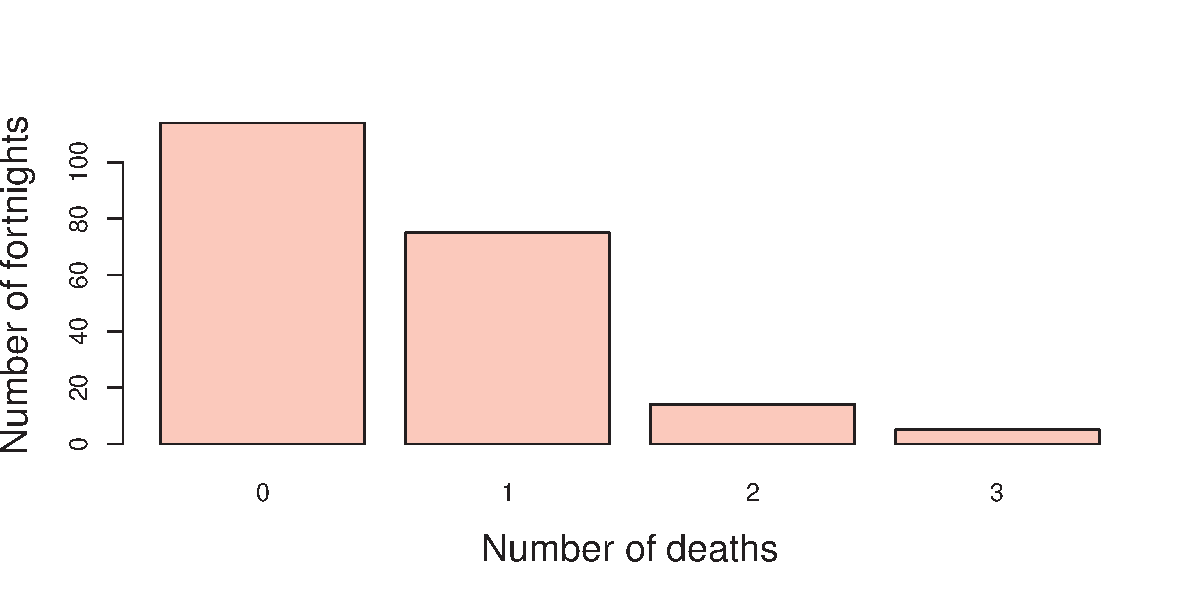
\includegraphics[width=.75\textwidth]{ch03/fig/cyclists2-1} }

\caption[Frequencies of number of cyclist deaths in two-week periods in London, 2005--2012]{Frequencies of number of cyclist deaths in two-week periods in London, 2005--2012\label{fig:cyclists2}}
\end{figure}


\end{knitrout}
We return to this data in \exref{ex:cyclists2} and answer the question of
how unusual six or more deaths would be in a Poisson distribution.

\end{Example}

\subsection{Type-token distributions}\label{sec:type-token}

There are a variety of other types of discrete data distributions.
One important class is \term{type-token} distributions, where
the basic count $k$ is the number of distinct types of some observed
event, $k = 1, 2, \dots$ and the frequency, $n_k$, is the number of
different instances observed.  For example, distinct words in a book,
words that subjects list as members of the semantic category ``fruit'',
musical notes that appear in a score, and species of animals caught
in traps can be considered as types, and the occurrences of
of those type comprise tokens.

This class differs from the Poisson type considered above
in that the frequency for value $k=0$ is \emph{unobserved}.  Thus, questions like
(a) How many words did Shakespeare know?
(b) How many words in the English language are members of the
``fruit'' category?
(c) How many wolves remain in Canada's Northwest territories?
depend on the unobserved count for $k=0$. They
cannot easily be answered without appeal to additional information
or statistical theory.


\begin{Example}[butterfly]{Butterfly species in Malaya}
In studies of the diversity of animal species, individuals are
collected and classified by species.
The distribution of the number of species (types) where $k = 1, 2, \dots$
individuals (tokens) were collected forms a kind of type-token distribution.
An early example of this kind of distribution was presented by
\citet{Fisher-etal:43}.
\tabref{tab:buttertab} lists the number of individuals of each of
501 species of butterfly collected in Malaya.
There were thus 118 species for which just a single instance was found,
74 species for which two individuals were found,
down to 3 species for which 24 individuals were collected.
Fisher et al.~note however that the distribution was truncated
at $k = 24$.
Type-token distributions are often J-shaped, with a long upper tail,
as we see in \figref{fig:butterfly}.
% latex table generated in R 3.0.1 by xtable 1.7-1 package
% Wed Nov 27 17:25:33 2013
%\begin{table}[ht]
%\centering
%\caption{Number of butterfly species $n_k$ for which $k$ individuals were collected} 
%\begin{tabular}{l|rrrrrrrrrrrrr rrrrrrrrrrrr}
%   \hline
%Individuals ($k$) & 1 & 2 & 3 & 4 & 5 & 6 & 7 & 8 & 9 & 10 & 11 & 12 
%                  & 13 & 14 & 15 & 16 & 17 & 18 & 19 & 20 & 21 & 22 & 23 & 24 & Sum \\ 
%   \hline
%Species ($n_k$) & 118 &  74 &  44 &  24 &  29 &  22 &  20 &  19 &  20 &  15 &  12 &  14 
%                &   6 &  12 &   6 &   9 &   9 &   6 &  10 &  10 &  11 &   5 &   3 &   3 & 501 \\ 
%  \end{tabular}
%\end{table}

%% hand edited to use two rows per line 
\begin{table}[ht]
\centering
\caption{Number of butterfly species $n_k$ for which $k$ individuals were collected} \label{tab:buttertab}
\begin{tabular}{l|rrrrrrrrrrrrr}
   \hline
Individuals ($k$) & 1 & 2 & 3 & 4 & 5 & 6 & 7 & 8 & 9 & 10 & 11 & 12 \\
Species ($n_k$)   & 118 &  74 &  44 &  24 &  29 &  22 &  20 &  19 &  20 &  15 &  12 &  14 \\
   \hline \hline
Individuals ($k$) & 13 & 14 & 15 & 16 & 17 & 18 & 19 & 20 & 21 & 22 & 23 & 24 & Sum \\ 
Species ($n_k$)   &   6 &  12 &   6 &   9 &   9 &   6 &  10 &  10 &  11 &   5 &   3 &   3 & 501 \\ 
   \hline
  \end{tabular}
\end{table}

 


\begin{knitrout}
\definecolor{shadecolor}{rgb}{1, 0.961, 0.933}\color{fgcolor}\begin{kframe}
\begin{alltt}
\hlstd{> }\hlkwd{data}\hlstd{(Butterfly,} \hlkwc{package} \hlstd{=} \hlstr{"vcd"}\hlstd{)}
\hlstd{> }\hlkwd{barplot}\hlstd{(Butterfly,} \hlkwc{xlab} \hlstd{=} \hlstr{"Number of individuals"}\hlstd{,} \hlkwc{ylab} \hlstd{=} \hlstr{"Number of species"}\hlstd{,}
\hlstd{+ }        \hlkwc{cex.lab} \hlstd{=} \hlnum{1.5}\hlstd{)}
\end{alltt}
\end{kframe}\begin{figure}[!htbp]

\centerline{\includegraphics[width=.9\textwidth]{ch03/fig/butterfly-1} }

\caption[Butterfly species in Malaya]{Butterfly species in Malaya\label{fig:butterfly}}
\end{figure}


\end{knitrout}

\end{Example}


\section{Characteristics of  discrete distributions}\label{sec:discrete-distrib}
This section briefly reviews the characteristics of some of the
important discrete distributions encountered in practice and illustrates their
use with \R.
An overview of these distributions is shown in \tabref{tab:distns}.
For more detailed information on these and other discrete distributions,
\citet{Johnson-etal:92} and \citet{WimmerAltman:1999:thesaurus}
present the most comprehensive treatments;
\citet[\C 2]{Zelterman:99} gives a compact summary.

\begin{table}[htbp]%
\caption{Discrete probability distributions\label{tab:distns}}%
\medskip
\small
\centering
\begin{tabular}{lll}\hline
Discrete          & Probability       & parameter(s)    \\ 
distribution      & function, $p(k)$  
\\ \hline
%
Binomial           & $\binom nk p^k(1-p)^{n-k}$       & \brk{$p$ = Pr
  (success);\\ $n$ = \# trials} \\[1ex] 
Poisson            & $e^{-\lambda }\lambda ^k/k!$     & $\lambda$ = mean  \\[1ex] 
Negative binomial  & $\binom{n+k-1}kp^n(1-p)^k$       &  $p$; $n$ = \#
\emph{successful} trials \\[1ex] 
Geometric          & $p(1-p)^k$                       &  $p$  \\[1ex]
Logarithmic series & $\theta ^k/[-k\log (1-\theta )]$ &  $\theta$ \\[1ex] \hline
\end{tabular}
\end{table}%



For each distribution, we describe properties and generating
mechanisms, and show how its parameters can be estimated
and how to plot the frequency distribution.  \R has a wealth of
functions for a wide variety of distributions.  For ease of reference,
their names and types for the distributions covered here are shown
in \tabref{tab:distfuns}. The naming scheme is simple and easy to
remember:  for each distribution, there are functions, with a prefix
letter, \code{d}, \code{p}, \code{q}, \code{r}, followed by the
name for that class of distribution:%
\footnote{The CRAN Task View on Probability Distributions,
\url{http://cran.r-project.org/web/views/Distributions.html},
provides a general overview and lists a wide variety of contributed
packages for specialized distributions, discrete and continuous.}
%\DONE{Resolved notation conflict here: I'm using $k$ for the number of successes, but \R functions use $x$.}
\begin{description*}
  \item[d] a density function,%
\footnote{
For discrete random variables this is usually called the probability mass function (pmf).
}
  $\Pr \{X = k\} \equiv p(k)$
for the probability that the variable $X$ takes the value $k$.
  \item[p] a cumulative probability function, or CDF,
  $F(k) = \sum_{X\le k} p(k)$.
  \item[q] a quantile function, the inverse of the CDF, $k = F^{-1} (p)$.
  The quantile  is defined as the smallest value $x$ such that $F(k) \ge p$.
  \item[r] a random number generating function for that distribution.
\end{description*}
In the \R console, \code{help(Distributions)} gives an overview listing of
the distribution functions available in the \Rpackage{stats}.

\begin{table}[htbp]%
\caption{\R functions for discrete probability distributions\label{tab:distfuns}}%
\medskip
%\small
\centering
\begin{tabular}{l|llll}
  \hline
  \tableheader
  \multilineL{Discrete\\distribution} & \multilineL{Density (pmf)\\function} 
          & \multilineL{Cumulative\\(CDF)} & \multilineL{Quantile\\CDF$^{-1}$} & \multilineL{Random \#\\generator} \\
%
%Discrete     & Density (pmf)    & Cumulative  & Quantile & Random \# \\ 
%distribution & function         & (CDF)       & CDF$^{-1}$    & generator \\  
\hline
%
Binomial          & \func{dbinom} & \func{pbinom} & \func{qbinom}  & \func{rbinom}  \\[0.5ex] 
Poisson           & \func{dpois} & \func{ppois} & \func{qpois}  & \func{rpois}  \\[0.5ex] 
Negative binomial & \func{dnbinom} & \func{pnbinom} & \func{qnbinom}  & \func{rnbinom}  \\[0.5ex] 
Geometric         & \func{dgeom} & \func{pgeom} & \func{qgeom}  & \func{rgeom}  \\[0.5ex]
Logarithmic series& \func{dlogseries} & \func{plogseries} & \func{qlogseries}  & \func{rlogseries}  \\[0.5ex]
\hline
\end{tabular}
\end{table}%




\subsection{The binomial distribution}\label{sec:binomial}
\ix{binomial distribution|(}
The binomial distribution, $\Bin(n, p)$,
arises as the distribution of the
number $k$ of events of interest which occur in $n$ independent trials
when the probability of the event on any one trial is the constant
value $p = \Pr ( \textrm{event} )$.
For example, if 15\% of the population has red hair,
the number of red-heads in randomly sampled groups of $n=10$
might follow a binomial distribution, $\Bin(10, 0.15)$;
in Weldon's dice data (\exref{ex:dice}), the probability of
a 5 or 6 should be $\frac13$ on any one trial, and
the number of 5s or 6s in tosses of 12 dice would follow
$\Bin(12, \frac13)$.

Over $n$ independent trials, the number of events  $k$
may range from 0 to $n$; if $X$ is a random variable
with a binomial distribution, the probability that $X = k$ is given
by
\begin{equation}\label{eq:binom}
\Bin(n,p): \Pr \{ X = k \} \equiv p ( k )  =
{n \choose k} p^k (1-p)^{n-k}
  \quad\quad k = 0, 1, \dots, n
  \comma
\end{equation}
where ${n \choose k} = n! / k! (n - k)!$ is the number of ways
of choosing $k$ out of $n$.
The first three (central) moments of the binomial distribution are
as follows
(letting $q = 1 - p$),
\begin{eqnarray*}
\textrm{Mean}(X) & = & n p  \\
\textrm{Var}(X) &  = & n p q \\
\textrm{Skew}(X) & = & n p q (q - p)
\period
\end{eqnarray*}
It is easy to verify that
the binomial distribution has its maximum variance when $p = \frac12$.
It is symmetric (Skew(x)=0) when $p = \frac12$, and negatively (positively)
skewed when $p < \frac12$ ($p > \frac12$ ).

If we are given data in the form of a discrete (binomial) distribution
(and $n$ is known),
then the maximum likelihood estimator of $p$ can be obtained
as the weighted mean of the values $k$ with weights $n_k$,
\begin{equation*}% \label{eq:binp}
\hat{p} = \frac{\bar{x}}{n} =
  \frac{(\sum_{k} k \times n_k ) / \sum_k n_k}{n}
  \comma
\end{equation*}
and has sampling variance $\V(\hat{p}) = pq/n$.

\TODO{DM: either add ref to some text explaining Maximum Likelihood estimation,
  or maybe add a section similar to old book to the Appendix), or add a note in preface
  that this is assumed to be known.}

\subsubsection{Calculation and visualization}
As indicated in \tabref{tab:distfuns} (but without listing the
parameters of these functions),
binomial probabilities
can be calculated with \code{dbinom(x, n, p)},
where \code{x} is a vector of the number of successes in \code{n}
trials and \code{p} is the probability of success on any one trial.
Cumulative probabilities, summed up to a vector of quantiles, \code{Q}
can be calculated with \code{pbinom(Q, n, p)},
and the quantiles (the smallest value $x$ such that $F(x) \ge P$)
with \code{qbinom(P, n, p)}.
To generate \code{N} random observations from a binomial distribution
with \code{n} trials and success probability \code{p}
use \code{rbinom(N, n, p)}\footnote{Note that the actual \R function
  arguments differ from the ones used here.}.


For example, to find and plot the binomial probabilities corresponding
to Weldon's tosses of 12 dice, with $k=0, \dots, 12$ and $p=\frac13$,
we could do the following
\begin{knitrout}
\definecolor{shadecolor}{rgb}{1, 0.961, 0.933}\color{fgcolor}\begin{kframe}
\begin{alltt}
\hlstd{> }\hlstd{k} \hlkwb{<-} \hlkwd{seq}\hlstd{(}\hlnum{0}\hlstd{,} \hlnum{12}\hlstd{)}
\hlstd{> }\hlstd{Pk} \hlkwb{<-} \hlkwd{dbinom}\hlstd{(k,} \hlnum{12}\hlstd{,} \hlnum{1}\hlopt{/}\hlnum{3}\hlstd{)}
\hlstd{> }\hlkwd{plot}\hlstd{(}\hlkwc{x} \hlstd{= k,} \hlkwc{y} \hlstd{= Pk,} \hlkwc{type} \hlstd{=} \hlstr{"h"}\hlstd{,}
\hlstd{+ }     \hlkwc{xlab} \hlstd{=} \hlstr{"Number of successes"}\hlstd{,} \hlkwc{ylab} \hlstd{=} \hlstr{"Probability"}\hlstd{,}
\hlstd{+ }     \hlkwc{lwd} \hlstd{=} \hlnum{8}\hlstd{,} \hlkwc{lend} \hlstd{=} \hlstr{"square"}\hlstd{)}
\hlstd{> }\hlkwd{lines}\hlstd{(}\hlkwc{x} \hlstd{= k,} \hlkwc{y} \hlstd{= Pk)}
\end{alltt}
\end{kframe}\begin{figure}[!htbp]

\centerline{\includegraphics[width=.75\textwidth]{ch03/fig/dbinom1-1} }

\caption[Binomial distribution for ]{Binomial distribution for $k=0,\dots,12$ successes in 12 trials and $p$=1/3\label{fig:dbinom1}}
\end{figure}


\end{knitrout}
\TODO{DM: Why not directly using a barplot?}
\begin{knitrout}
\definecolor{shadecolor}{rgb}{1, 0.961, 0.933}\color{fgcolor}\begin{kframe}
\begin{alltt}
\hlstd{> }\hlstd{k} \hlkwb{<-} \hlnum{0} \hlopt{:} \hlnum{12}
\hlstd{> }\hlstd{Pk} \hlkwb{<-} \hlkwd{dbinom}\hlstd{(k,} \hlnum{12}\hlstd{,} \hlnum{1}\hlopt{/}\hlnum{3}\hlstd{)}
\hlstd{> }\hlstd{b} \hlkwb{<-} \hlkwd{barplot}\hlstd{(Pk,} \hlkwc{names.arg} \hlstd{= k,}
\hlstd{+ }             \hlkwc{xlab} \hlstd{=} \hlstr{"Number of successes"}\hlstd{,} \hlkwc{ylab} \hlstd{=} \hlstr{"Probability"}\hlstd{)}
\hlstd{> }\hlkwd{lines}\hlstd{(}\hlkwc{x} \hlstd{= b,} \hlkwc{y} \hlstd{= Pk,} \hlkwc{col} \hlstd{=} \hlstr{"red"}\hlstd{)}
\end{alltt}
\end{kframe}\begin{figure}[!htbp]

\centerline{\includegraphics[width=.75\textwidth]{ch03/fig/dbinom12-1} }

\caption[Binomial distribution for ]{Binomial distribution for $k=0,\dots,12$ successes in 12 trials and $p$=1/3\label{fig:dbinom12}}
\end{figure}


\end{knitrout}
Note that in the call to \func{plot}, \code{type = "h"} draws histogram-typed
lines to the bottom of the vertical axis, and \code{lwd = 8} makes them wide.
The call to \func{lines} shows another way to plot the data, as a probability
polygon. We illustrate other styles for plotting in \secref{sec:poisson},
\exref{ex:dpois-plot} below.

\begin{Example}[dice2]{Weldon's dice}
Going a bit further, we can compare Weldon's data with the
theoretical binomial distribution as shown below. Because the
\data{WeldonDice} data collapsed the frequencies for 10--12
successes as $10+$,
we do the same with the binomial probabilities.
The expected frequencies (\code{Exp}), if Weldon's dice tosses obeyed
the binomial distribution, are calculated as $N \times p(k)$ for
$N=26,306$ tosses.  In addition, we compute the differences of
the observed (\code{Freq}) and expected (\code{Exp}) frequencies as
column \code{Diff}, to be used for the $\chisq$ test for goodness of fit
described later in \secref{sec:discrete-fit}, but a glance
these are all negative for
$k=0, \dots 4$ and positive thereafter.

\begin{knitrout}
\definecolor{shadecolor}{rgb}{1, 0.961, 0.933}\color{fgcolor}\begin{kframe}
\begin{alltt}
\hlstd{> }\hlstd{Weldon_df} \hlkwb{<-} \hlkwd{as.data.frame}\hlstd{(WeldonDice)} \hlcom{# convert to data frame}
\hlstd{> }
\hlstd{> }\hlstd{k} \hlkwb{<-} \hlnum{0} \hlopt{:} \hlnum{12}                       \hlcom{# same as seq(0, 12)}
\hlstd{> }\hlstd{Pk} \hlkwb{<-} \hlkwd{dbinom}\hlstd{(k,} \hlnum{12}\hlstd{,} \hlnum{1}\hlopt{/}\hlnum{3}\hlstd{)}          \hlcom{# binomial probabilities}
\hlstd{> }\hlstd{Pk} \hlkwb{<-} \hlkwd{c}\hlstd{(Pk[}\hlnum{1}\hlopt{:}\hlnum{10}\hlstd{],} \hlkwd{sum}\hlstd{(Pk[}\hlnum{11}\hlopt{:}\hlnum{13}\hlstd{]))} \hlcom{# sum values for 10+}
\hlstd{> }\hlstd{Exp} \hlkwb{<-} \hlkwd{round}\hlstd{(}\hlnum{26306} \hlopt{*} \hlstd{Pk)}          \hlcom{# expected frequencies}
\hlstd{> }\hlstd{Diff} \hlkwb{<-} \hlstd{Weldon_df}\hlopt{$}\hlstd{Freq} \hlopt{-} \hlstd{Exp}      \hlcom{# raw residuals}
\hlstd{> }\hlstd{Chisq} \hlkwb{<-} \hlstd{Diff}\hlopt{^}\hlnum{2} \hlopt{/} \hlstd{Exp}
\hlstd{> }\hlkwd{data.frame}\hlstd{(Weldon_df,} \hlkwc{Prob} \hlstd{=} \hlkwd{round}\hlstd{(Pk,} \hlnum{5}\hlstd{), Exp, Diff, Chisq)}
\end{alltt}
\begin{verbatim}
   n56 Freq    Prob  Exp Diff   Chisq
1    0  185 0.00771  203  -18 1.59606
2    1 1149 0.04624 1216  -67 3.69161
3    2 3265 0.12717 3345  -80 1.91330
4    3 5475 0.21195 5576 -101 1.82945
5    4 6114 0.23845 6273 -159 4.03013
6    5 5194 0.19076 5018  176 6.17298
7    6 3067 0.11127 2927  140 6.69628
8    7 1331 0.04769 1255   76 4.60239
9    8  403 0.01490  392   11 0.30867
10   9  105 0.00331   87   18 3.72414
11 10+   18 0.00054   14    4 1.14286
\end{verbatim}
\end{kframe}
\end{knitrout}
\end{Example}

Finally, we can use programming features in \R to calculate and plot
probabilities for binomial distributions over a range of
both \code{k} and \code{p} as follows, for the purposes of
graphing the distributions as one or both varies.
The following code uses \func{expand.grid} to create a data frame \code{KP}
containing all combinations of \code{k = 0:12} and
\code{p = c(1/6, 1/3, 1/2, 2/3)}. These values are then supplied as
arguments to \func{dbinom}.  For the purpose of plotting,
the decimal value of \code{p} is declared as a factor.

\begin{knitrout}
\definecolor{shadecolor}{rgb}{1, 0.961, 0.933}\color{fgcolor}\begin{kframe}
\begin{alltt}
\hlstd{> }\hlstd{KP} \hlkwb{<-} \hlkwd{expand.grid}\hlstd{(}\hlkwc{k} \hlstd{=} \hlnum{0} \hlopt{:} \hlnum{12}\hlstd{,} \hlkwc{p} \hlstd{=} \hlkwd{c}\hlstd{(}\hlnum{1}\hlopt{/}\hlnum{6}\hlstd{,} \hlnum{1}\hlopt{/}\hlnum{3}\hlstd{,} \hlnum{1}\hlopt{/}\hlnum{2}\hlstd{,} \hlnum{2}\hlopt{/}\hlnum{3}\hlstd{))}
\hlstd{> }\hlstd{bin_df} \hlkwb{<-} \hlkwd{data.frame}\hlstd{(KP,} \hlkwc{prob} \hlstd{=} \hlkwd{dbinom}\hlstd{(KP}\hlopt{$}\hlstd{k,} \hlnum{12}\hlstd{, KP}\hlopt{$}\hlstd{p))}
\hlstd{> }\hlstd{bin_df}\hlopt{$}\hlstd{p} \hlkwb{<-} \hlkwd{factor}\hlstd{(bin_df}\hlopt{$}\hlstd{p,} \hlkwc{labels} \hlstd{=} \hlkwd{c}\hlstd{(}\hlstr{"1/6"}\hlstd{,} \hlstr{"1/3"}\hlstd{,} \hlstr{"1/2"}\hlstd{,} \hlstr{"2/3"}\hlstd{))}
\hlstd{> }\hlkwd{str}\hlstd{(bin_df)}
\end{alltt}
\begin{verbatim}
'data.frame':	52 obs. of  3 variables:
 $ k   : int  0 1 2 3 4 5 6 7 8 9 ...
 $ p   : Factor w/ 4 levels "1/6","1/3","1/2",..: 1 1 1 1 1 1 1 1 1 1 ...
 $ prob: num  0.1122 0.2692 0.2961 0.1974 0.0888 ...
\end{verbatim}
\end{kframe}
\end{knitrout}

This data can be plotted using \func{xyplot} in \pkg{lattice},
using the \code{groups} argument to make separate curves for each
value of \code{p}.  The following code generates \figref{fig:dbinom2-plot}.
\begin{knitrout}
\definecolor{shadecolor}{rgb}{1, 0.961, 0.933}\color{fgcolor}\begin{kframe}
\begin{alltt}
\hlstd{> }\hlkwd{library}\hlstd{(lattice)}
\hlstd{> }\hlstd{mycol} \hlkwb{<-} \hlkwd{palette}\hlstd{()[}\hlnum{2}\hlopt{:}\hlnum{5}\hlstd{]}
\hlstd{> }\hlkwd{xyplot}\hlstd{(prob} \hlopt{~} \hlstd{k,} \hlkwc{data} \hlstd{= bin_df,} \hlkwc{groups} \hlstd{= p,}
\hlstd{+ }  \hlkwc{xlab} \hlstd{=} \hlkwd{list}\hlstd{(}\hlstr{"Number of successes"}\hlstd{,} \hlkwc{cex} \hlstd{=} \hlnum{1.25}\hlstd{),}
\hlstd{+ }  \hlkwc{ylab} \hlstd{=} \hlkwd{list}\hlstd{(}\hlstr{"Probability"}\hlstd{,}  \hlkwc{cex} \hlstd{=} \hlnum{1.25}\hlstd{),}
\hlstd{+ }  \hlkwc{type} \hlstd{=} \hlstr{"b"}\hlstd{,} \hlkwc{pch} \hlstd{=} \hlnum{15}\hlopt{:}\hlnum{17}\hlstd{,} \hlkwc{lwd} \hlstd{=} \hlnum{2}\hlstd{,} \hlkwc{cex} \hlstd{=} \hlnum{1.25}\hlstd{,} \hlkwc{col} \hlstd{= mycol,}
\hlstd{+ }  \hlkwc{key} \hlstd{=} \hlkwd{list}\hlstd{(}
\hlstd{+ }    \hlkwc{title} \hlstd{=} \hlstr{"Pr(success)"}\hlstd{,}
\hlstd{+ }    \hlkwc{points} \hlstd{=} \hlkwd{list}\hlstd{(}\hlkwc{pch} \hlstd{=} \hlnum{15} \hlopt{:} \hlnum{17}\hlstd{,} \hlkwc{col} \hlstd{= mycol,} \hlkwc{cex} \hlstd{=} \hlnum{1.25}\hlstd{),}
\hlstd{+ }    \hlkwc{lines} \hlstd{=} \hlkwd{list}\hlstd{(}\hlkwc{lwd} \hlstd{=} \hlnum{2}\hlstd{,} \hlkwc{col} \hlstd{= mycol),}
\hlstd{+ }    \hlkwc{text} \hlstd{=} \hlkwd{list}\hlstd{(}\hlkwd{levels}\hlstd{(bin_df}\hlopt{$}\hlstd{p)),}
\hlstd{+ }    \hlkwc{x} \hlstd{=} \hlnum{0.9}\hlstd{,} \hlkwc{y} \hlstd{=} \hlnum{0.98}\hlstd{,} \hlkwc{corner} \hlstd{=} \hlkwd{c}\hlstd{(}\hlkwc{x} \hlstd{=} \hlnum{1}\hlstd{,} \hlkwc{y} \hlstd{=} \hlnum{1}\hlstd{)}
\hlstd{+ }    \hlstd{)}
\hlstd{+ }  \hlstd{)}
\end{alltt}
\end{kframe}\begin{figure}[!htbp]

\centerline{\includegraphics[width=.75\textwidth]{ch03/fig/dbinom2-plot-1} }

\caption[Binomial distributions for ]{Binomial distributions for $k=0, \dots, 12$ successes in $n=12$ trials, and four values of $p$\label{fig:dbinom2-plot}}
\end{figure}


\end{knitrout}

\TODO{DM: Avoid lattice to reduce complexity. Either only use ggplot2
  throughout the chpater,
  or use base graphics here, and ggplot2 for the remaining plots:}

\begin{knitrout}
\definecolor{shadecolor}{rgb}{1, 0.961, 0.933}\color{fgcolor}\begin{kframe}
\begin{alltt}
\hlstd{> }\hlstd{p} \hlkwb{<-} \hlkwd{c}\hlstd{(}\hlnum{1}\hlopt{/}\hlnum{6}\hlstd{,} \hlnum{1}\hlopt{/}\hlnum{3}\hlstd{,} \hlnum{1}\hlopt{/}\hlnum{2}\hlstd{,} \hlnum{2}\hlopt{/}\hlnum{3}\hlstd{)}
\hlstd{> }\hlstd{k} \hlkwb{<-} \hlnum{0} \hlopt{:} \hlnum{12}
\hlstd{> }\hlstd{Prob} \hlkwb{<-} \hlkwd{outer}\hlstd{(k, p,} \hlkwa{function}\hlstd{(}\hlkwc{k}\hlstd{,} \hlkwc{p}\hlstd{)} \hlkwd{dbinom}\hlstd{(k,} \hlnum{12}\hlstd{, p))}
\hlstd{> }\hlkwd{str}\hlstd{(Prob)}
\end{alltt}
\begin{verbatim}
 num [1:13, 1:4] 0.1122 0.2692 0.2961 0.1974 0.0888 ...
\end{verbatim}
\end{kframe}
\end{knitrout}

\begin{knitrout}
\definecolor{shadecolor}{rgb}{1, 0.961, 0.933}\color{fgcolor}\begin{kframe}
\begin{alltt}
\hlstd{> }\hlstd{col} \hlkwb{<-} \hlkwd{palette}\hlstd{()[}\hlnum{2}\hlopt{:}\hlnum{5}\hlstd{]}
\hlstd{> }\hlkwd{matplot}\hlstd{(k, Prob,}
\hlstd{+ }        \hlkwc{type} \hlstd{=} \hlstr{"o"}\hlstd{,} \hlkwc{pch} \hlstd{=} \hlnum{15} \hlopt{:} \hlnum{17}\hlstd{,} \hlkwc{col} \hlstd{= col,} \hlkwc{lty} \hlstd{=} \hlnum{1}\hlstd{,}
\hlstd{+ }        \hlkwc{xlab} \hlstd{=} \hlstr{"Number of Successes"}\hlstd{,} \hlkwc{ylab} \hlstd{=} \hlstr{"Probability"}\hlstd{)}
\hlstd{> }\hlkwd{legend}\hlstd{(}\hlstr{"topright"}\hlstd{,} \hlkwc{legend} \hlstd{=} \hlkwd{c}\hlstd{(}\hlstr{"1/6"}\hlstd{,}\hlstr{"1/3"}\hlstd{,}\hlstr{"1/2"}\hlstd{,}\hlstr{"2/3"}\hlstd{),}
\hlstd{+ }       \hlkwc{pch} \hlstd{=} \hlnum{15} \hlopt{:} \hlnum{17}\hlstd{,} \hlkwc{lty} \hlstd{=} \hlnum{1}\hlstd{,} \hlkwc{col} \hlstd{= col,} \hlkwc{title} \hlstd{=} \hlstr{"Pr(Success)"}\hlstd{)}
\end{alltt}
\end{kframe}\begin{figure}[!htbp]

\centerline{\includegraphics[width=.75\textwidth]{ch03/fig/dbinom2-plot2-1} }

\caption[Binomial distributions for ]{Binomial distributions for $k=0, \dots, 12$ successes in $n=12$ trials, and four values of $p$\label{fig:dbinom2-plot2}}
\end{figure}


\end{knitrout}

\ix{binomial distribution|)}  % end index on

\subsection{The Poisson distribution}\label{sec:poisson}
\ix{Poisson distribution|(}

The Poisson distribution gives the probability of an event occurring
$k = 0, 1, 2, \dots$ times over a large number of independent ``trials'',
when the probability, $p$, that the event occurs on any one
trial (in time or space) is small and constant.
Hence, the Poisson distribution is usually applied to the study of
rare events such as highway accidents at a particular location,
deaths from horse kicks, or defects in a well-controlled manufacturing
process.  Other applications include:
the number of customers contacting a call center per unit time;
the number of insurance claims per unit region or unit time;
number of particles emitted from a small radioactive sample.

For the \IX{Poisson distribution}, the probability function
is
\begin{equation}\label{eq:poisf}
\Pois(\lambda):\Pr \{ X = k \} \equiv p (k)=
  \frac{ e^{ - \lambda } \:  \lambda^k } { k ! }
  \quad\quad k = 0, 1, \dots
\end{equation}
where the rate parameter, $\lambda$ ($>0$), turns out to be the mean of the
distribution.
The first three (central) moments of the Poisson distribution are:
%in fact all equal to $\lambda$:
\begin{eqnarray*}
\textrm{Mean}(X) & = & \lambda \\
\textrm{Var}(X) &  = & \lambda \\
\textrm{Skew}(X) & = & \lambda^{- 1/2}
\end{eqnarray*}
%% Mathematica gives Skew = 1 / \sqrt(\lambda) ???

So, the mean and variance of the Poisson distribution are always
the same, which is sometimes used to identify a distribution
as Poisson.  For the binomial distribution, the mean ($Np$) is always
greater than the variance ($Npq$); for other distributions
(negative binomial and geometric) the mean is less than the
variance. The Poisson distribution is always positively skewed,
but skewness decreases as $\lambda$ increases.

The maximum likelihood estimator of the parameter \(\lambda\)
in \eqref{eq:poisf} is just
the mean of the distribution,
\begin{equation}
  \hat{\lambda}= \bar{x} = \frac{\sum_k k \,  n_k}{\sum_k  n_k} \label{eq:pois-lambda}
  \period
\end{equation}
Hence, the expected frequencies can be estimated by substituting the
sample mean into \eqref{eq:poisf} and multiplying by the total
sample size $N$.

There are many useful properties of the Poisson distribution.%
\TODO{DM: Better add some book ref? Wikipedia is not persistent ...}
\footnote{
See: \url{http://en.wikipedia.org/wiki/Poisson_distribution}
}
Among these:
\begin{itemize*}
  \item Poisson variables have a nice reproductive property:
    if $X_1, X_2, \dots X_m$ are independent Poisson
    variables with the same parameter $\lambda$, then their
    sum, $\sum X_i$ is a Poisson variate with parameter $m \lambda$;
    if the Poisson parameters differ, the sum is still Poisson with
    parameter $\sum \lambda_i$.
  \item For two or more independent Poisson variables,
    $X_1 \sim \Pois(\lambda_1), X_2 \sim \Pois(\lambda_2), \dots$, with rate parameters
    $ \lambda_1, \lambda_2 \dots$, the distribution of
    any $X_i$, \emph{conditional on their sum}, $\sum_j X_j = n$, is
    binomial, $\Bin (n, p)$, where $p = \lambda_i / \sum_j \lambda_j$.
  \item As $\lambda$ increases, the Poisson distribution becomes increasingly
    symmetric, and approaches the normal distribution $N (\lambda, \lambda)$
    with mean and variance $\lambda$ as $\lambda \rightarrow \infty$.
    The approximation is quite good with $\lambda > 20$.
  \item If $X \sim \Pois(\lambda)$, then $\sqrt{X}$ converges much faster to
    a normal distribution $N (\lambda, \frac14)$, with mean $\sqrt\lambda$
    and constant variance $\frac14$.  Hence, the square root transformation is often recommended
    as a \emph{variance stabilizing} transformation for count data
    when classical methods (ANOVA, regression) assuming normality are employed.
  \end{itemize*}


\begin{Example}[soccer]{UK Soccer scores}
\tabref{tab:soccer1}  gives the distributions of goals scored by
the 20 teams in the  1995/96 season of the
 Premier League of the UK Football Association
as presented originally by
\citet{Lee:97}, and now available as the two-way table \data{UKSoccer}
in the \Rpackage{vcd}.
\begin{table}[!t]
\caption{Goals scored by home and away teams in 380 games in the Premier
Football League, 1995/96 season}
\label{tab:soccer1}
\begin{center}
\vspace{.1in}
\begin{tabular}{r|rrrrr|r}
  \hline
Home      & \multicolumn{5}{c|}{Away Team Goals} \\
Team      &       0 &      1 &       2&       3&      4+&  Total \\
Goals     &  \multicolumn{5}{c|}{}   \\
  \hline
			0 &     27 &     29 &     10 &      8 &      2 &     76 \\
			1 &     59 &     53 &     14 &     12 &      4 &    142 \\
			2 &     28 &     32 &     14 &     12 &      4 &     90 \\
			3 &     19 &     14 &      7 &      4 &      1 &     45 \\
			4+&      7 &      8 &     10 &      2 &      0 &     27 \\
  \hline
Total      &  140   &    136 &     55 &     38 &     11 &    380 \\
  \hline
\end{tabular}
\end{center}
\end{table}
Over a season
each team plays each other team exactly once, so there are a total of
$20 \times 19 = 380$ games.
Because there may be an advantage for the home team,
the goals scored have been classified as ``home team'' goals
and ``away team'' goals in the table. Of interest for this example is whether
the number of goals scores by home teams and away teams follow
Poisson distributions, and how this relates to the distribution of the
total number of goals scored.

If we assume that in any small interval of time there is a small, constant
probability that the home team or the away team may score a goal,
the distributions of the goals scored by home teams
(the row totals in \tabref{tab:soccer1})
may be modeled as Pois($\lambda_H$) and the distribution of
the goals scored by away teams (the column totals)
may be modeled as Pois($\lambda_A$).

If the number of goals scored by the home and away teams are independent%
\footnote{This question
is examined visually in \chref{ch:mosaic} (\exref{ex:soccer2})
and \chref{ch:corresp} (\exref{ex:soccer3}), where we find that the answer
is ``basically, yes''.},
we would expect that the total number of goals scored in any
game would be distributed as Pois($\lambda_H + \lambda_A$).
These totals are shown in \tabref{tab:soccer2}.
\begin{table}[!hb]
\caption{Total goals scored in 380 games in the Premier
Football League, 1995/95 season}
\label{tab:soccer2}
\vspace{.1in}
\begin{center}
\begin{tabular}{l|rrrr rrrr}
\hline
Total goals      &  0  &  1  &  2  &  3  &  4  &  5  &  6  &  7  \\
\hline
Number of games  & 27  & 88  & 91  & 73  & 49  & 31  & 18  &  3  \\
  \hline
\end{tabular}
\end{center}
\end{table}


As a preliminary check of the distributions for the home and away goals,
we can determine if the means and variances are reasonably close
to each other.
If so, then the total goals variable should also have a mean and variance
equal to the sum of those statistics for the home and away goals.

In the \R code below, we first convert the two-way frequency table
\data{UKSoccer} to a data frame in frequency form.
We use \func{within} to convert \var{Home} and \var{Away} to
numeric variables, and calculate \var{Total} as their sum.

\begin{knitrout}
\definecolor{shadecolor}{rgb}{1, 0.961, 0.933}\color{fgcolor}\begin{kframe}
\begin{alltt}
\hlstd{> }\hlkwd{data}\hlstd{(UKSoccer,} \hlkwc{package} \hlstd{=} \hlstr{"vcd"}\hlstd{)}
\hlstd{> }
\hlstd{> }\hlstd{soccer.df} \hlkwb{<-} \hlkwd{as.data.frame}\hlstd{(UKSoccer,} \hlkwc{stringsAsFactors} \hlstd{=} \hlnum{FALSE}\hlstd{)}
\hlstd{> }\hlstd{soccer.df} \hlkwb{<-} \hlkwd{within}\hlstd{(soccer.df, \{}
\hlstd{+ }  \hlstd{Home} \hlkwb{<-} \hlkwd{as.numeric}\hlstd{(Home)}       \hlcom{# make numeric}
\hlstd{+ }  \hlstd{Away} \hlkwb{<-} \hlkwd{as.numeric}\hlstd{(Away)}       \hlcom{# make numeric}
\hlstd{+ }  \hlstd{Total} \hlkwb{<-} \hlstd{Home} \hlopt{+} \hlstd{Away}           \hlcom{# total goals}
\hlstd{+ }\hlstd{\})}
\hlstd{> }\hlkwd{str}\hlstd{(soccer.df)}
\end{alltt}
\begin{verbatim}
'data.frame':	25 obs. of  4 variables:
 $ Home : num  0 1 2 3 4 0 1 2 3 4 ...
 $ Away : num  0 0 0 0 0 1 1 1 1 1 ...
 $ Freq : num  27 59 28 19 7 29 53 32 14 8 ...
 $ Total: num  0 1 2 3 4 1 2 3 4 5 ...
\end{verbatim}
\end{kframe}
\end{knitrout}
To calculate the mean and variance of these variables, first expand
the data frame to 380 individual observations using \func{expand.dft}.
Then use \func{apply} over the rows to calculate the mean and variance
in each column.
\begin{knitrout}
\definecolor{shadecolor}{rgb}{1, 0.961, 0.933}\color{fgcolor}\begin{kframe}
\begin{alltt}
\hlstd{> }\hlstd{soccer.df} \hlkwb{<-} \hlkwd{expand.dft}\hlstd{(soccer.df)}   \hlcom{# expand to ungrouped form}
\hlstd{> }\hlkwd{apply}\hlstd{(soccer.df,} \hlnum{2}\hlstd{,} \hlkwc{FUN} \hlstd{=} \hlkwa{function}\hlstd{(}\hlkwc{x}\hlstd{)} \hlkwd{c}\hlstd{(}\hlkwc{mean} \hlstd{=} \hlkwd{mean}\hlstd{(x),} \hlkwc{var} \hlstd{=} \hlkwd{var}\hlstd{(x)))}
\end{alltt}
\begin{verbatim}
       Home   Away  Total
mean 1.4868 1.0632 2.5500
var  1.3164 1.1728 2.6175
\end{verbatim}
\end{kframe}
\end{knitrout}

The means are all approximately equal to the corresponding variances.
More to the point, the variance of the \texttt{Total} score
is approximately equal to the sum of the individual variances.
Note also there does appear to be an advantage for the home team,
of nearly half a goal.

\end{Example}

\begin{Example}[cyclists2]{London cycling deaths}
A quick check of whether the numbers of deaths among London cyclists
follows the Poisson distribution
can be carried out by calculating the mean and variance.
The \term{index of dispersion}, the ratio of the variance to the mean,
is commonly used to quantify whether a set of observed frequencies
is more or less dispersed than a reference (Poisson) distribution.
\begin{knitrout}
\definecolor{shadecolor}{rgb}{1, 0.961, 0.933}\color{fgcolor}\begin{kframe}
\begin{alltt}
\hlstd{> }\hlkwd{with}\hlstd{(CyclingDeaths,} \hlkwd{c}\hlstd{(}\hlkwc{mean} \hlstd{=} \hlkwd{mean}\hlstd{(deaths),}
\hlstd{+ }                      \hlkwc{var} \hlstd{=} \hlkwd{var}\hlstd{(deaths),}
\hlstd{+ }                      \hlkwc{ratio} \hlstd{=} \hlkwd{mean}\hlstd{(deaths)} \hlopt{/} \hlkwd{var}\hlstd{(deaths)))}
\end{alltt}
\begin{verbatim}
   mean     var   ratio 
0.56731 0.52685 1.07679 
\end{verbatim}
\end{kframe}
\end{knitrout}
Thus, there was an average of about
0.57
deaths per fortnight,
or a bit more than 1 per month, and no evidence for over- or 
underdispersion.

We can now answer the question of whether it was an extraordinary
event to observe six deaths in a two-week period, by calculating
the probability of more than 5 deaths using \func{ppois}.
\begin{knitrout}
\definecolor{shadecolor}{rgb}{1, 0.961, 0.933}\color{fgcolor}\begin{kframe}
\begin{alltt}
\hlstd{> }\hlstd{mean.deaths} \hlkwb{<-} \hlkwd{mean}\hlstd{(CyclingDeaths}\hlopt{$}\hlstd{deaths)}
\hlstd{> }\hlkwd{ppois}\hlstd{(}\hlnum{5}\hlstd{, mean.deaths,} \hlkwc{lower.tail} \hlstd{=} \hlnum{FALSE}\hlstd{)}
\end{alltt}
\begin{verbatim}
[1] 2.8543e-05
\end{verbatim}
\end{kframe}
\end{knitrout}
This probability is extremely small, so we conclude that the
occurrence of six deaths was a singular event.
The interpretation of this result might indicate an increased
risk to cycling in London, and might prompt further study of
road safety.
\end{Example}


\subsubsection{Calculation and visualization}
For the Poisson distribution, you can generate probabilities using
\code{dpois(x, lambda)} for the numbers of events in \code{x} with
rate parameter \code{lambda}. As we did earlier for the binomial
distribution, we can calculate these for a collection of values
of \code{lambda} by using \func{expand.grid} to create all combinations
of with the values of \code{x} we wish to plot.

\begin{Example}[dpois-plot]{Plotting styles for discrete distributions}
In this example, we illustrate some additional styles for plotting discrete
distributions, using both \pkg{lattice} \func{xyplot} and the
\Rpackage{ggplot2}.  The goal here is to visualize a collection of
Poisson distributions for varying values of $\lambda$.

We first create the 63 combinations of \code{x = 0 : 20} for
three values of $\lambda$, \code{lambda = c(1, 4, 10)}, and use these
columns as arguments to \func{dpois}.  Again, \code{lambda} is
a numeric variable, but the plotting methods are easier if this
variable is converted to a factor.
\begin{knitrout}
\definecolor{shadecolor}{rgb}{1, 0.961, 0.933}\color{fgcolor}\begin{kframe}
\begin{alltt}
\hlstd{> }\hlstd{KL} \hlkwb{<-} \hlkwd{expand.grid}\hlstd{(}\hlkwc{k} \hlstd{=} \hlnum{0} \hlopt{:} \hlnum{20}\hlstd{,} \hlkwc{lambda} \hlstd{=} \hlkwd{c}\hlstd{(}\hlnum{1}\hlstd{,} \hlnum{4}\hlstd{,} \hlnum{10}\hlstd{))}
\hlstd{> }\hlstd{pois_df} \hlkwb{<-} \hlkwd{data.frame}\hlstd{(KL,} \hlkwc{prob} \hlstd{=} \hlkwd{dpois}\hlstd{(KL}\hlopt{$}\hlstd{k, KL}\hlopt{$}\hlstd{lambda))}
\hlstd{> }\hlstd{pois_df}\hlopt{$}\hlstd{lambda} \hlkwb{=} \hlkwd{factor}\hlstd{(pois_df}\hlopt{$}\hlstd{lambda)}
\hlstd{> }\hlkwd{str}\hlstd{(pois_df)}
\end{alltt}
\begin{verbatim}
'data.frame':	63 obs. of  3 variables:
 $ k     : int  0 1 2 3 4 5 6 7 8 9 ...
 $ lambda: Factor w/ 3 levels "1","4","10": 1 1 1 1 1 1 1 1 1 1 ...
 $ prob  : num  0.3679 0.3679 0.1839 0.0613 0.0153 ...
\end{verbatim}
\end{kframe}
\end{knitrout}

Discrete distributions are often plotted as bar charts or in histogram-like
form, as we did for the examples in \secref{sec:discrete-intro},
rather than the line-graph form used for the binomial distribution in
\figref{fig:dbinom2-plot}.  With \func{xyplot}, the plot style is controlled
by the \code{type} argument, and the code below uses \code{type = c("h", "p")}
to get \emph{both} histogram-like lines to the origin and points.
As well, the plot formula, \code{prob ~ k | lambda} instructs \func{xyplot}
to produce a multi-panel plot, conditioned on values of \code{lambda}.
These lines produce \figref{fig:dpois-xyplot1}.

\begin{knitrout}
\definecolor{shadecolor}{rgb}{1, 0.961, 0.933}\color{fgcolor}\begin{kframe}
\begin{alltt}
\hlstd{> }\hlkwd{xyplot}\hlstd{(prob} \hlopt{~} \hlstd{k} \hlopt{|} \hlstd{lambda,} \hlkwc{data} \hlstd{= pois_df,}
\hlstd{+ }  \hlkwc{type} \hlstd{=} \hlkwd{c}\hlstd{(}\hlstr{"h"}\hlstd{,} \hlstr{"p"}\hlstd{),} \hlkwc{pch} \hlstd{=} \hlnum{16}\hlstd{,} \hlkwc{lwd} \hlstd{=} \hlnum{4}\hlstd{,} \hlkwc{cex} \hlstd{=} \hlnum{1.25}\hlstd{,} \hlkwc{layout} \hlstd{=} \hlkwd{c}\hlstd{(}\hlnum{3}\hlstd{,} \hlnum{1}\hlstd{),}
\hlstd{+ }  \hlkwc{xlab} \hlstd{=} \hlkwd{list}\hlstd{(}\hlstr{"Number of events (k)"}\hlstd{,} \hlkwc{cex} \hlstd{=} \hlnum{1.25}\hlstd{),}
\hlstd{+ }  \hlkwc{ylab} \hlstd{=} \hlkwd{list}\hlstd{(}\hlstr{"Probability"}\hlstd{,} \hlkwc{cex} \hlstd{=} \hlnum{1.25}\hlstd{))}
\end{alltt}
\end{kframe}\begin{figure}[!htbp]

\centerline{\includegraphics[width=\textwidth]{ch03/fig/dpois-xyplot1-1} }

\caption[Poisson distributions for ]{Poisson distributions for $\lambda$ = 1, 4, 10, in a multi-panel display\label{fig:dpois-xyplot1}}
\end{figure}


\end{knitrout}

The line-graph plot style of \figref{fig:dbinom2-plot} has the advantage that
it is easier to compare the separate distributions in a single plot
(using the \code{groups} argument) than
across multiple panels (using a conditioning formula).
It has the disadvantages that (a) a proper legend is
difficult to construct with \pkg{lattice}, and (b) is difficult to read, because
you have to visually coordinate the curves in the plot with the values shown
in the legend.  \figref{fig:dpois-xyplot2} solves both problems using
the \Rpackage{directlabels}.
\begin{knitrout}
\definecolor{shadecolor}{rgb}{1, 0.961, 0.933}\color{fgcolor}\begin{kframe}
\begin{alltt}
\hlstd{> }\hlstd{mycol} \hlkwb{<-} \hlkwd{palette}\hlstd{()[}\hlnum{2}\hlopt{:}\hlnum{4}\hlstd{]}
\hlstd{> }\hlstd{plt} \hlkwb{<-} \hlkwd{xyplot}\hlstd{(prob} \hlopt{~} \hlstd{k,} \hlkwc{data} \hlstd{= pois_df,} \hlkwc{groups} \hlstd{= lambda,}
\hlstd{+ }  \hlkwc{type} \hlstd{=} \hlstr{"b"}\hlstd{,} \hlkwc{pch} \hlstd{=} \hlnum{15} \hlopt{:} \hlnum{17}\hlstd{,} \hlkwc{lwd} \hlstd{=} \hlnum{2}\hlstd{,} \hlkwc{cex} \hlstd{=} \hlnum{1.25}\hlstd{,} \hlkwc{col} \hlstd{= mycol,}
\hlstd{+ }  \hlkwc{xlab} \hlstd{=} \hlkwd{list}\hlstd{(}\hlstr{"Number of events (k)"}\hlstd{,} \hlkwc{cex} \hlstd{=} \hlnum{1.25}\hlstd{),}
\hlstd{+ }  \hlkwc{ylab} \hlstd{=} \hlkwd{list}\hlstd{(}\hlstr{"Probability"}\hlstd{,}  \hlkwc{cex} \hlstd{=} \hlnum{1.25}\hlstd{))}
\hlstd{> }	
\hlstd{> }\hlkwd{library}\hlstd{(directlabels)}
\hlstd{> }\hlkwd{direct.label}\hlstd{(plt,} \hlkwd{list}\hlstd{(}\hlstr{"top.points"}\hlstd{,} \hlkwc{cex} \hlstd{=} \hlnum{1.5}\hlstd{,} \hlkwd{dl.trans}\hlstd{(}\hlkwc{y} \hlstd{= y} \hlopt{+} \hlnum{0.1}\hlstd{)))}
\end{alltt}
\end{kframe}\begin{figure}[!htbp]

\centerline{\includegraphics[width=.8\textwidth]{ch03/fig/dpois-xyplot2-1} }

\caption[Poisson distributions for ]{Poisson distributions for $\lambda$ = 1, 4, 10, using direct labels\label{fig:dpois-xyplot2}}
\end{figure}


\end{knitrout}
Note that the plot constructed by \func{xyplot} is saved as a
(\class{trellis}) object, \code{plt}.  The function
\func{direct.label}
massages this to add the labels directly to each curve.  In the
second argument above, \code{"top.points"} says to locate these
at the maximum value on each curve.

Finally, we illustrate the use of \pkg{ggplot2} to produce a single-panel,
multi-line plot of these distributions. The basic plot uses
\code{aes(x = k, y = prob, ...)} to produce a plot of \code{prob} vs. \code{k},
assigning color and shape attributes to the values of \code{lambda}.

\begin{knitrout}
\definecolor{shadecolor}{rgb}{1, 0.961, 0.933}\color{fgcolor}\begin{kframe}
\begin{alltt}
\hlstd{> }\hlkwd{library}\hlstd{(ggplot2)}
\hlstd{> }\hlstd{gplt} \hlkwb{<-} \hlkwd{ggplot}\hlstd{(pois_df,} \hlkwd{aes}\hlstd{(}\hlkwc{x} \hlstd{= k,} \hlkwc{y} \hlstd{= prob,} \hlkwc{colour} \hlstd{= lambda,} \hlkwc{shape} \hlstd{= lambda))} \hlopt{+}
\hlstd{+ }  \hlkwd{geom_line}\hlstd{(}\hlkwc{size} \hlstd{=} \hlnum{1}\hlstd{)} \hlopt{+} \hlkwd{geom_point}\hlstd{(}\hlkwc{size} \hlstd{=} \hlnum{3}\hlstd{)} \hlopt{+}
\hlstd{+ }        \hlkwd{xlab}\hlstd{(}\hlstr{"Number of events (k)"}\hlstd{)} \hlopt{+}
\hlstd{+ }        \hlkwd{ylab}\hlstd{(}\hlstr{"Probability"}\hlstd{)}
\end{alltt}
\end{kframe}
\end{knitrout}
\pkg{ggplot2} allows most details of the plot to be modified using
\func{theme}.  Here we use this to move the legend inside the plot,
and enlarge the axis labels and titles.
\begin{knitrout}
\definecolor{shadecolor}{rgb}{1, 0.961, 0.933}\color{fgcolor}\begin{kframe}
\begin{alltt}
\hlstd{> }\hlstd{gplt} \hlopt{+} \hlkwd{theme}\hlstd{(}\hlkwc{legend.position} \hlstd{=} \hlkwd{c}\hlstd{(}\hlnum{0.8}\hlstd{,} \hlnum{0.8}\hlstd{))} \hlopt{+}  \hlcom{# manually move legend}
\hlstd{+ }       \hlkwd{theme}\hlstd{(}\hlkwc{axis.text} \hlstd{=} \hlkwd{element_text}\hlstd{(}\hlkwc{size} \hlstd{=} \hlnum{12}\hlstd{),}
\hlstd{+ }             \hlkwc{axis.title} \hlstd{=} \hlkwd{element_text}\hlstd{(}\hlkwc{size} \hlstd{=} \hlnum{14}\hlstd{,} \hlkwc{face} \hlstd{=} \hlstr{"bold"}\hlstd{))}
\end{alltt}
\end{kframe}\begin{figure}[!htbp]

\centerline{\includegraphics[width=.8\textwidth]{ch03/fig/dpois-ggplot2-1} }

\caption[Poisson distributions for ]{Poisson distributions for $\lambda$ = 1, 4, 10, using ggplot\label{fig:dpois-ggplot2}}
\end{figure}


\end{knitrout}

\end{Example}

\ix{Poisson distribution|)}

\subsection{The negative binomial distribution}\label{sec:negbin}
\ix{negative binomial distribution|(}

The negative binomial distribution is a type of waiting-time distribution,
but also arises in statistical applications as a generalization of the
Poisson distribution, allowing for \term{overdispersion} (variance > mean).
See \citet{Hilbe:2011:negbin} for a comprehensive treatment
of negative binomial statistical models with many applications in \R.

One form of
the negative binomial distribution
(also called the \term{Pascal distribution}) arises when a series of
independent Bernoulli
trials is observed with constant probability $p$ of some event,
and we ask how many non-events (failures), $k$, it takes to observe
$n$ successful events.  For example, in tossing one die repeatedly,
we may consider the outcome ``1'' as a ``success'' (with $p=\frac16$)
and ask about the probability of observing $k = 0, 1, 2, \dots$
failures before getting $n=3$ 1s.


The probability function with parameters $n$ (a positive integer, $0 < n < \infty$) and $p \, (0 < p < 1)$
gives the probability that $k$ non-events (failures) are observed before
the $n$-th event (success), and
can be written%
\footnote{
There are a variety of other parameterizations of the negative binomial distribution,
but all of these can be converted to the form shown here, which is relatively
standard, and consistent with \R. They differ in whether the parameter $n$
relates to the number of successes or the total number of trials, and
whether the stopping criterion is defined in terms of failures or successes.
See: \url{http://en.wikipedia.org/wiki/Negative_binomial_distribution}
for details on these variations.
}
\begin{equation}\label{eq:negbinf}
\NBin(n,p):   \Pr \{ X = k \} \equiv p(k)  =
  {n+k-1 \choose k} p^n (1-p)^k
  \quad\quad k = 0, 1, \dots , \infty
\end{equation}
This formulation makes clear that a given sequence of events involves
a total of $n+k$ trials of which there are $n$ successes,
with probability $p^n$, and $k$ are failures, with probability $(1-p)^k$.
The binomial coefficient, ${n+k-1 \choose k}$ gives the number of ways
to choose the $k$ successes from the remaining $n+k-1$ trials preceding
the last success.

The first three central moments of the negative binomial distribution are:
\begin{eqnarray*}
\textrm{Mean}(X) &=&nq / p  = \mu \\
\textrm{Var}(X) &=&nq / p^2 \\
\textrm{Skew}(X) &=&\frac{2-p}{\sqrt{nq}}
\comma
\end{eqnarray*}
where $q=1-p$. The variance of $X$ is therefore greater than the mean,
and the distribution is always positively skewed.

A more general form of the negative binomial distribution
(the \term{Polya distribution})
allows $n$ to take non-integer values and to be an unknown
parameter.
In this case, the combinatorial coefficient,
${n+k-1 \choose k}$ in \eqref{eq:negbinf} is calculated using
the gamma function, $\Gamma(\bullet)$,
a generalization of the factorial for non-integer values,
defined so that $\Gamma(x+1) = x!$ when $x$ is an integer.

Then the probability function \eqref{eq:negbinf} becomes
\begin{equation}\label{eq:negbinf2}
  \Pr \{ X = k \} \equiv p(k)  =
  \frac{\Gamma(n+k)}{\Gamma(n) \Gamma(k+1)}
   p^n (1-p)^k
  \quad\quad k = 0, 1, \dots , \infty
  \period
\end{equation}

\citet{GreenwoodYule:20}
developed the negative binomial distribution as a model for
accident proneness or susceptibility of individuals to
repeated attacks of disease.
They assumed that for any individual, $i$, the number of accidents
or disease occurrences has a Poisson distribution with parameter
$\lambda_i$.
If individuals vary in proneness, so that the $\lambda_i$ have
a gamma distribution, the resulting distribution is the
negative binomial.

In this form, the negative binomial distribution is frequently used
as an alternative to the Poisson distribution when the assumptions
of the Poisson (constant probability and independence) are not
satisfied, or when the variance of the distribution is greater
than the mean (overdispersion).
This gives rise to an alternative parameterization in terms of the
mean ($\mu$) of the distribution and its relation to the variance.
From the relation of the mean and variance to the parameters
$n, p$ given above,

\begin{eqnarray}
\textrm{Mean}(X) = \mu = \frac{n (1-p)}{p} & \implies & p = \frac{n}{n+\mu} \\
\textrm{Var}(X) = \frac{n (1-p)}{p^2} & \implies & \textrm{Var}(X) = \mu + \frac{\mu^2}{n}
\end{eqnarray}
This formulation allows the variance of the distribution to exceed the mean,
and in these terms, the ``size'' parameter $n$ is called the
\term{dispersion parameter}.%
\footnote{
Other terms are ``shape parameter,'' with reference to the mixing distribution
of Poissons with varying $\lambda$,
``heterogeneity parameter,'' or ``aggregation parameter.''
}
Increasing this parameter corresponds to less heterogeneity, variance closer
to the mean, and therefore greater applicability of the Poisson distribution.

\subsubsection{Calculation and visualization}

In \R, the density (pmf), distribution (CDF), quantile and random number functions
for the negative binomial distribution are a bit special, in that the parameterization
can be specified using either $(n, p)$ or $(n, \mu)$ forms,
where $\mu = n (1-p) /p$.
In our notation, probabilities can be calculated using \func{dnbinom}
using the call \code{dbinom(k, n, p)}
or the call \code{dbinom(k, n, mu=)}, as illustrated below:

\begin{knitrout}
\definecolor{shadecolor}{rgb}{1, 0.961, 0.933}\color{fgcolor}\begin{kframe}
\begin{alltt}
\hlstd{> }\hlstd{k} \hlkwb{<-} \hlnum{2}
\hlstd{> }\hlstd{n} \hlkwb{<-} \hlnum{2} \hlopt{:} \hlnum{4}
\hlstd{> }\hlstd{p} \hlkwb{<-} \hlnum{0.2}
\hlstd{> }\hlkwd{dnbinom}\hlstd{(k, n, p)}
\end{alltt}
\begin{verbatim}
[1] 0.07680 0.03072 0.01024
\end{verbatim}
\begin{alltt}
\hlstd{> }\hlstd{(mu} \hlkwb{<-} \hlstd{n} \hlopt{*} \hlstd{(}\hlnum{1} \hlopt{-} \hlstd{p)} \hlopt{/} \hlstd{p)}
\end{alltt}
\begin{verbatim}
[1]  8 12 16
\end{verbatim}
\begin{alltt}
\hlstd{> }\hlkwd{dnbinom}\hlstd{(k, n,} \hlkwc{mu} \hlstd{= mu)}
\end{alltt}
\begin{verbatim}
[1] 0.07680 0.03072 0.01024
\end{verbatim}
\end{kframe}
\end{knitrout}
Thus, for the distribution with \code{k = 2} failures and
 \code{n = 2 : 4} successes with probability \code{p = 0.2},
the values \code{n = 2:4} correspond to means $\mu= 8, 12, 16$
as shown above.

As before, we can calculate these probabilities for a range
of the combinations of arguments using \func{expand.grid}.
In the example below,
we allow three values for each of \code{n} and \code{p}
and calculate all probabilities for all values of \code{k}
from 0 to 20. The result, \code{nbin_df} is like a 3-way,
$21 \times 3 \times 3$
array of \code{prob} values, but in data frame format.
\begin{knitrout}
\definecolor{shadecolor}{rgb}{1, 0.961, 0.933}\color{fgcolor}\begin{kframe}
\begin{alltt}
\hlstd{> }\hlstd{XN} \hlkwb{<-} \hlkwd{expand.grid}\hlstd{(}\hlkwc{k} \hlstd{=} \hlnum{0} \hlopt{:} \hlnum{20}\hlstd{,} \hlkwc{n} \hlstd{=} \hlkwd{c}\hlstd{(}\hlnum{2}\hlstd{,} \hlnum{4}\hlstd{,} \hlnum{6}\hlstd{),} \hlkwc{p} \hlstd{=} \hlkwd{c}\hlstd{(}\hlnum{0.2}\hlstd{,} \hlnum{0.3}\hlstd{,} \hlnum{0.4}\hlstd{))}
\hlstd{> }\hlstd{nbin_df} \hlkwb{<-} \hlkwd{data.frame}\hlstd{(XN,} \hlkwc{prob} \hlstd{=} \hlkwd{dnbinom}\hlstd{(XN}\hlopt{$}\hlstd{k, XN}\hlopt{$}\hlstd{n, XN}\hlopt{$}\hlstd{p))}
\hlstd{> }\hlstd{nbin_df}\hlopt{$}\hlstd{n} \hlkwb{<-} \hlkwd{factor}\hlstd{(nbin_df}\hlopt{$}\hlstd{n)}
\hlstd{> }\hlstd{nbin_df}\hlopt{$}\hlstd{p} \hlkwb{<-} \hlkwd{factor}\hlstd{(nbin_df}\hlopt{$}\hlstd{p)}
\hlstd{> }\hlkwd{str}\hlstd{(nbin_df)}
\end{alltt}
\begin{verbatim}
'data.frame':	189 obs. of  4 variables:
 $ k   : int  0 1 2 3 4 5 6 7 8 9 ...
 $ n   : Factor w/ 3 levels "2","4","6": 1 1 1 1 1 1 1 1 1 1 ...
 $ p   : Factor w/ 3 levels "0.2","0.3","0.4": 1 1 1 1 1 1 1 1 1 1 ...
 $ prob: num  0.04 0.064 0.0768 0.0819 0.0819 ...
\end{verbatim}
\end{kframe}
\end{knitrout}

With 9 combinations of the parameters, it is most convenient
to plot these in separate panels, in a $3 \times 3$ display.
The formula \code{prob ~ k | n + p} in the call to
\func{xyplot} constructs plots of
\code{prob} vs. \code{k} conditioned on the combinations of
\code{n} and \code{p}.
\begin{knitrout}
\definecolor{shadecolor}{rgb}{1, 0.961, 0.933}\color{fgcolor}\begin{kframe}
\begin{alltt}
\hlstd{> }\hlkwd{xyplot}\hlstd{(prob} \hlopt{~} \hlstd{k} \hlopt{|} \hlstd{n} \hlopt{+} \hlstd{p,} \hlkwc{data} \hlstd{= nbin_df,}
\hlstd{+ }  \hlkwc{xlab} \hlstd{=} \hlkwd{list}\hlstd{(}\hlstr{"Number of failures (k)"}\hlstd{,} \hlkwc{cex} \hlstd{=} \hlnum{1.25}\hlstd{),}
\hlstd{+ }  \hlkwc{ylab} \hlstd{=} \hlkwd{list}\hlstd{(}\hlstr{"Probability"}\hlstd{,}  \hlkwc{cex} \hlstd{=} \hlnum{1.25}\hlstd{),}
\hlstd{+ }  \hlkwc{type} \hlstd{=} \hlkwd{c}\hlstd{(}\hlstr{"h"}\hlstd{,} \hlstr{"p"}\hlstd{),} \hlkwc{pch} \hlstd{=} \hlnum{16}\hlstd{,} \hlkwc{lwd} \hlstd{=} \hlnum{2}\hlstd{,}
\hlstd{+ }  \hlkwc{strip} \hlstd{=} \hlkwd{strip.custom}\hlstd{(}\hlkwc{strip.names} \hlstd{=} \hlnum{TRUE}\hlstd{)}
\hlstd{+ }        \hlstd{)}
\end{alltt}
\end{kframe}\begin{figure}[!htbp]

\centerline{\includegraphics[width=.85\textwidth]{ch03/fig/dnbin3-1} }

\caption[Negative binomial distributions for ]{Negative binomial distributions for $n = 2, 4, 6$ and $p=0.2, 0.3, 0.4$, using xyplot\label{fig:dnbin3}}
\end{figure}


\end{knitrout}
%\TODO{Modify \figref{fig:dnbin3} to show the mean and standard deviation}

It can be readily seen that the mean increases from left to
right with \code{n}, and increases from top to bottom with
decreasing \code{p}.  For these distributions, we can also
calculate the theory-implied means, $\mu$, across the entire
distributions, $k = 0, 1, \dots \infty$, as shown below.

\begin{knitrout}
\definecolor{shadecolor}{rgb}{1, 0.961, 0.933}\color{fgcolor}\begin{kframe}
\begin{alltt}
\hlstd{> }\hlstd{NP} \hlkwb{<-} \hlkwd{expand.grid}\hlstd{(}\hlkwc{n}\hlstd{=}\hlkwd{c}\hlstd{(}\hlnum{2}\hlstd{,} \hlnum{4}\hlstd{,} \hlnum{6}\hlstd{),} \hlkwc{p}\hlstd{=}\hlkwd{c}\hlstd{(}\hlnum{0.2}\hlstd{,} \hlnum{0.3}\hlstd{,} \hlnum{0.4}\hlstd{))}
\hlstd{> }\hlstd{NP} \hlkwb{<-} \hlkwd{within}\hlstd{(NP, \{ mu} \hlkwb{=} \hlstd{n}\hlopt{*}\hlstd{(}\hlnum{1}\hlopt{-}\hlstd{p)}\hlopt{/}\hlstd{p \})}
\hlstd{> }\hlcom{# show as matrix}
\hlstd{> }\hlkwd{matrix}\hlstd{(NP}\hlopt{$}\hlstd{mu,} \hlnum{3}\hlstd{,} \hlnum{3}\hlstd{,} \hlkwc{dimnames}\hlstd{=}\hlkwd{list}\hlstd{(}\hlkwc{n}\hlstd{=}\hlkwd{c}\hlstd{(}\hlnum{2}\hlstd{,}\hlnum{4}\hlstd{,}\hlnum{6}\hlstd{),} \hlkwc{p}\hlstd{=(}\hlnum{2}\hlopt{:}\hlnum{4}\hlstd{)}\hlopt{/}\hlnum{10}\hlstd{))}
\end{alltt}
\begin{verbatim}
   p
n   0.2     0.3 0.4
  2   8  4.6667   3
  4  16  9.3333   6
  6  24 14.0000   9
\end{verbatim}
\end{kframe}
\end{knitrout}

\TODO{DM: maybe simpler?}

\begin{knitrout}
\definecolor{shadecolor}{rgb}{1, 0.961, 0.933}\color{fgcolor}\begin{kframe}
\begin{alltt}
\hlstd{> }\hlstd{n} \hlkwb{<-} \hlkwd{c}\hlstd{(}\hlnum{2}\hlstd{,} \hlnum{4}\hlstd{,} \hlnum{6}\hlstd{)}
\hlstd{> }\hlstd{p} \hlkwb{<-} \hlkwd{c}\hlstd{(}\hlnum{0.2}\hlstd{,} \hlnum{0.3}\hlstd{,} \hlnum{0.4}\hlstd{)}
\hlstd{> }\hlstd{NP} \hlkwb{<-} \hlkwd{outer}\hlstd{(n, p,} \hlkwa{function}\hlstd{(}\hlkwc{n}\hlstd{,} \hlkwc{p}\hlstd{) n} \hlopt{*} \hlstd{(}\hlnum{1} \hlopt{-} \hlstd{p)} \hlopt{/} \hlstd{p)}
\hlstd{> }\hlkwd{dimnames}\hlstd{(NP)} \hlkwb{<-} \hlkwd{list}\hlstd{(}\hlkwc{n} \hlstd{= n,} \hlkwc{p} \hlstd{= p)}
\hlstd{> }\hlstd{NP}
\end{alltt}
\begin{verbatim}
   p
n   0.2     0.3 0.4
  2   8  4.6667   3
  4  16  9.3333   6
  6  24 14.0000   9
\end{verbatim}
\end{kframe}
\end{knitrout}

\ix{negative binomial distribution|)}

\subsection{The geometric distribution}\label{sec:geometric}
\ix{geometric distribution|(}
The special case of the negative binomial distribution when $n=1$
is a geometric distribution.
We observe a series of independent trials and count the number
of non-events (failures) preceding the first successful event.
The probability that there will be  $k$ failures before the first
success
is given by
\begin{equation}\label{eq:geomf}
\Geom(p):   \Pr \{ X = k \} \equiv p ( k )  =
   p (1-p)^k
  \quad\quad k = 0, 1, \dots
  \period
\end{equation}
For this distribution the central moments are:
\begin{eqnarray*}
\textrm{Mean}(X) & = & 1 / p\\
\textrm{Var}(X) &  = & (1-p) / p^2 \\
\textrm{Skew}(X) & = & (2-p) / \sqrt{1-p}
\end{eqnarray*}

Note that estimation of the parameter $p$ for the geometric distribution
can be handled as the special case of the negative binomial by fixing $n=1$,
so no special software is needed.
Going the other way, if $X_1, X_2, \dots X_n$ are independent geometrically
distributed as $\Geom(p)$, then their sum, $Y = \sum_j^n X_j$ is distributed
as $\NBin(p, n)$.

In \R, the standard set of functions for the geometric distribution are
available as
\code{dgeom(x, prob)},
\code{pgeom(q, prob)},
\code{qgeom(p, prob)} and
\code{rgeom(n, prob)} where \code{prob} represents $p$ here.
Visualization of the geometric distribution follows the pattern used earlier
for other discrete distributions.

\ix{geometric distribution|)}

\subsection{The logarithmic series distribution}
\ix{logarithmic series distribution|(}
The logarithmic series distribution is a long-tailed distribution
introduced by
\citet{Fisher-etal:43}
in connection with data on the abundance of individuals
classified by species of the type shown for the distribution of butterfly
species
in \tabref{tab:buttertab}.

The probability distribution function with parameter $p$ is given by
\begin{equation}\label{eq:logseriesf}
\textrm{LogSer}(p): \Pr \{ X = k \} \equiv p ( k )  =
\frac{p^k}{-(k\log (1-p ))} =
\alpha \, p^k / k
\quad\quad k = 1, 2, \dots, \infty
\comma
\end{equation}
where $\alpha = -1 / \log(1 - p)$
and $0 < p <1$.
For this distribution, the first two central moments are:
\begin{eqnarray*}
\textrm{Mean}(X) & = & \alpha \left(\frac{p}{1-p}\right)\\
\textrm{Var}(X) &  = & -p \frac{p + \log(1-p)}{(1-p)^2 \log^2(1-p)}\\
\end{eqnarray*}


Fisher derived the logarithmic series distribution by assuming that
for a given species the number of individuals trapped has a Poisson
distribution with parameter $\lambda = \gamma t$, where
$\gamma$ is a parameter of the species (susceptibility to entrapment)
and $t$ is a parameter of the trap.
If different species vary so that the parameter $\gamma$ has a gamma
distribution, then the number of representatives of each species trapped
will have a negative binomial distribution.
However, the observed distribution is necessarily truncated on the left,
because one cannot observe the number of species never caught (where $k=0$).
The logarithmic series distribution thus arises as a limiting form of the
zero-truncated negative binomial.

Maximum likelihood estimation of the parameter $p$ in the log-series
distribution is described by \citet{Bohning:1983}, extending a simpler
Newton's method approximation by \citet{Birch:63}.
The \Rpackage{vcdExtra} contains the
set of \R functions,
\code{dlogseries(x, prob)},
\code{plogseries(q, prob)},
\code{qlogseries(p, prob)} and
\code{rlogseries(n, prob)} where \code{prob} represents $p$ here.


\TODO{implement the log-series in \func{goodfit} and \func{distplot} so this distribution
can be used in later sections.}


\ix{logarithmic series distribution|)}

\subsection{Power series family}\label{sec:pwrseries}
\ix{power series distributions|(}

We mentioned earlier that the Poisson distribution was unique among all discrete (one parameter) distributions, in that it is the only one whose mean and variance are equal
\citep{Kosambi:49}.
The relation between mean and variance of discrete distributions also provides
the basis for integrating them into a general family.
All of the discrete distributions described in this section are in fact
special cases of a family of discrete distributions
called the power series distributions by
\citet{Noack:50}
and defined by
\begin{equation*}
p(k) = a(k) \theta^k / f(\theta)
\quad\quad k=0, 1, \dots \comma
\end{equation*}
with parameter $\theta > 0$,
where $a(k)$ is a coefficient function depending only on $k$
and $f ( \theta) = \sum_k a(k) \theta^k$ is called the series
function.  The definitions of these functions are shown in
\tabref{tab:pwrseries}.
\begin{table}[!tb] \centering%
\caption{The Power Series family of discrete distributions\label{tab:pwrseries}}%
\small
\begin{tabular}{lllll}\hline
Discrete & Probability  & Series  & Series  & Series \\ 
Distributiion & function, $p(k)$ & parameter, $\theta$ &
function, $f(\theta )$ & coefficient, $a(k)$ \\ \hline
%
Poisson & $e^{-\lambda }\lambda ^k/k!$ & $\theta = \lambda$ & $e^\theta $ & $1/k!$ \\[1ex] 
Binomial & $\binom nkp^k(1-p)^{n-k}$ & $\theta = p / (1-p) $ & $(1+\theta )^n$ & $\binom nk$ \\[1ex] 
Negative binomial & $\binom{n+k-1}kp^n(1-p)^k$ &  $\theta = (1-p) $ & $(1-\theta )^{-k}$ & $%
\binom{n+k-1}k$ \\[1ex] 
Geometric & $p(1-p)^k$ &  $\theta = (1-p)$ & $(1-\theta )^{-k}$ & $1$ \\[1ex]
Logarithmic series & $\theta ^k/[-k\log (1-\theta )]$ &  $\theta = \theta$ & $-\log (1-\theta )$
& $1/k$ \\[1ex] \hline
\end{tabular}
%TCIMACRO{\TeXButton{E}{\end{table}}}
%BeginExpansion
\end{table}%
%EndExpansion



These relations among the discrete distribution provide the basis for
graphical techniques for diagnosing the form of discrete data described
later in this chapter (\secref{sec:discrete-other}).
\ix{power series distributions|)}


\section{Fitting discrete distributions}\label{sec:discrete-fit}

In applications to discrete data such as the examples in
\secref{sec:discrete-intro}, interest is often focused on how closely such data follow a
particular distribution, such as the Poisson, binomial, or geometric
distribution.  A close fit provides for interpretation in terms
of the underlying mechanism for the distribution;  conversely, a
bad fit can suggest the possibility for improvement by relaxing
one or more of the assumptions. We examine more detailed and
nuanced methods for diagnosing and testing discrete distributions
in \secref{sec:discrete-ord} and \secref{sec:discrete-Poissonness}
below.

Fitting a discrete distribution involves three basic steps:
\begin{enumerate*}

\item Estimating the parameter(s) of the distribution from the
data, for example, $p$ for the binomial, $\lambda$ for the
Poisson, $n$ and $p$ for the negative binomial. Typically,
this is carried out by maximum likelihood methods, or a simpler
method of moments, which equates sample moments (mean, variance, skewness) to those of the theoretical distribution, and solves
for the parameter estimates.  These methods are illustrated in \secref{sec:fitdistr}.

\item  From this, we can calculate the fitted probabilities,
$\hat{p}_k$ that apply for the given distribution,
or equivalently, the model expected frequencies,
$N \hat{p}_k$, where $N$ is the total sample size.

\item Finally, we can calculate goodness-of-fit tests
measuring the departure between the observed and
fitted frequencies.
\end{enumerate*}

Often goodness-of-fit is examined with a classical (Pearson)
\term{goodness-of-fit} (GOF) chi-squared test,
%\glosstex{chi-square test}

\begin{equation}\label{eq:chi2}
  X^2 = \sum_{k=1}^K \:
  \frac{{ ( n_k - N \hat{p}_k ) }^2}
  { N \hat{p}_k }  \sim \chi^2_{( K-s-1 )}
  \comma
\end{equation}
where there are $K$ frequency classes,
$s$ parameters have been estimated from the data and
\(\hat{p}_k\) is the estimated probability of each basic count,
under the null hypothesis that the data follows the chosen distribution.

An alternative test statistic is the likelihood-ratio $G^2$
statistic,
\begin{equation}\label{eq:g2}
 G^2 = \sum_{k=1}^K \: n_k \log ( n_k / N \hat{p}_k )
 \comma
\end{equation}
when the $\hat{p}_k$ are estimated by maximum likelihood,
which also has an asymptotic $\chi^2_{(K - s - 1)}$ distribution.
``Asymptotic'' means that these are \emph{large sample tests},
meaning that the test statistic follows the $\chi^2$ distribution
increasingly well as $N \rightarrow \infty$.
A common rule of thumb is that all \emph{expected} frequencies
should exceed one and that fewer than 20\% should be less than 5.

\begin{Example}[horsekick2]{Death by horse kick}
We illustrate the basic ideas of goodness-of fit tests
with the \data{HorseKick} data, where we expect a Poisson
distribution with parameter $\lambda$ = mean number of
deaths. As shown in \eqref{eq:pois-lambda}, this is calculated
as the frequency ($n_k$) weighted mean of the $k$ values,
here, number of deaths.

In \R, such one-way frequency distributions should be converted
to data frames with numeric variables. The calculation below
uses \func{weighted.mean} with the frequencies as weights,
and finds $\lambda = 0.61$ as the mean number of deaths per
corps-year.
\begin{knitrout}
\definecolor{shadecolor}{rgb}{1, 0.961, 0.933}\color{fgcolor}\begin{kframe}
\begin{alltt}
\hlstd{> }\hlcom{# goodness-of-fit test}
\hlstd{> }\hlstd{tab} \hlkwb{<-} \hlkwd{as.data.frame}\hlstd{(HorseKicks,} \hlkwc{stringsAsFactors} \hlstd{=} \hlnum{FALSE}\hlstd{)}
\hlstd{> }\hlkwd{colnames}\hlstd{(tab)} \hlkwb{<-} \hlkwd{c}\hlstd{(}\hlstr{"nDeaths"}\hlstd{,} \hlstr{"Freq"}\hlstd{)}
\hlstd{> }\hlkwd{str}\hlstd{(tab)}
\end{alltt}
\begin{verbatim}
'data.frame':	5 obs. of  2 variables:
 $ nDeaths: chr  "0" "1" "2" "3" ...
 $ Freq   : int  109 65 22 3 1
\end{verbatim}
\begin{alltt}
\hlstd{> }\hlstd{(lambda} \hlkwb{<-} \hlkwd{weighted.mean}\hlstd{(}\hlkwd{as.numeric}\hlstd{(tab}\hlopt{$}\hlstd{nDeaths),} \hlkwc{w} \hlstd{= tab}\hlopt{$}\hlstd{Freq))}
\end{alltt}
\begin{verbatim}
[1] 0.61
\end{verbatim}
\end{kframe}
\end{knitrout}

From this, we can calculate the probabilities (\code{phat})
of \code{k = 0 : 4}
deaths, and hence the expected (\code{exp}) frequencies in a
Poisson distribution.

\begin{knitrout}
\definecolor{shadecolor}{rgb}{1, 0.961, 0.933}\color{fgcolor}\begin{kframe}
\begin{alltt}
\hlstd{> }\hlstd{phat} \hlkwb{<-} \hlkwd{dpois}\hlstd{(}\hlnum{0} \hlopt{:} \hlnum{4}\hlstd{,} \hlkwc{lambda} \hlstd{= lambda)}
\hlstd{> }\hlstd{exp} \hlkwb{<-} \hlkwd{sum}\hlstd{(tab}\hlopt{$}\hlstd{Freq)} \hlopt{*} \hlstd{phat}
\hlstd{> }\hlstd{chisq} \hlkwb{<-} \hlstd{(tab}\hlopt{$}\hlstd{Freq} \hlopt{-} \hlstd{exp)}\hlopt{^}\hlnum{2} \hlopt{/} \hlstd{exp}
\hlstd{> }
\hlstd{> }\hlstd{GOF} \hlkwb{<-} \hlkwd{data.frame}\hlstd{(tab, phat, exp, chisq)}
\hlstd{> }\hlstd{GOF}
\end{alltt}
\begin{verbatim}
  nDeaths Freq      phat       exp     chisq
1       0  109 0.5433509 108.67017 0.0010011
2       1   65 0.3314440  66.28881 0.0250573
3       2   22 0.1010904  20.21809 0.1570484
4       3    3 0.0205551   4.11101 0.3002534
5       4    1 0.0031346   0.62693 0.2220057
\end{verbatim}
\end{kframe}
\end{knitrout}
Finally, the Pearson $\chi^2$ is just the sum of the \code{chisq}
values and \func{pchisq} is used to calculate the
$p$-value of this test statistic---the probability of obtaining this
$\chi^2$ or a more extreme value if our assumption on the
underlying distribution is true. 

\begin{knitrout}
\definecolor{shadecolor}{rgb}{1, 0.961, 0.933}\color{fgcolor}\begin{kframe}
\begin{alltt}
\hlstd{> }\hlkwd{sum}\hlstd{(chisq)}  \hlcom{# chi-square value}
\end{alltt}
\begin{verbatim}
[1] 0.70537
\end{verbatim}
\begin{alltt}
\hlstd{> }\hlkwd{pchisq}\hlstd{(}\hlkwd{sum}\hlstd{(chisq),} \hlkwc{df} \hlstd{=} \hlkwd{nrow}\hlstd{(tab)} \hlopt{-} \hlnum{2}\hlstd{,} \hlkwc{lower.tail} \hlstd{=} \hlnum{FALSE}\hlstd{)}
\end{alltt}
\begin{verbatim}
[1] 0.87194
\end{verbatim}
\end{kframe}
\end{knitrout}
The result, $\chi^2_3$ = 0.70537 shows an
extremely good fit of these data to the Poisson distribution,
perhaps exceptionally so.%
\footnote{
An exceptionally good fit occurs when the $p$-value for
the test $\chi^2$ statistic is so high, as to suggest
that something unreasonable under random sampling might have
occurred.  The classic example of this is the
controversy over Gregor Mendel's experiments of cross-breeding
garden peas with various observed (phenotype) characteristics,
where R. A. Fisher \citeyearpar{Fisher:1936:Mendel} suggested that
observed frequencies of combinations like (smooth/wrinkled),
(green/yellow) in a 2$^{nd}$ generation were uncomfortably too
close to the $3:1$ ratio predicted by genetic theory.
}

\end{Example}

\subsection[R tools for discrete distributions]{\R tools for discrete distributions}\label{sec:fitdistr}
In \R, the function \func{fitdistr} in the \pkg{MASS}
is a basic work horse for fitting a variety of distributions
by maximum likelihood and other methods, giving parameter estimates
and standard errors.
Among discrete distributions, the binomial,
Poisson and geometric distributions have closed-form
maximum likelihood estimates; the negative binomial distribution,
parameterized by ($n, \mu$), is estimated iteratively by direct
optimization.

These basic calculations are extended and enhanced for one-way
discrete distributions in the \pkg{vcd} function
\func{goodfit}, which
computes the fitted values of a discrete distribution (either Poisson, binomial or negative binomial) to the count data.
If the parameters are not specified they are estimated either by ML or Minimum Chi-squared. \func{print} and \func{summary} methods for
the \class{goodfit} objects give, respectively, a table of
observed and fitted frequencies, and the Pearson and/or likelihood
ratio goodness-of-fit statistics. Plotting methods for visualizing
the discrepancies between observed and fitted frequencies are
described and illustrated in \secref{sec:fitplot}.

\begin{Example}[saxfit]{Families in Saxony}
This example uses \func{goodfit} to fit the binomial
to the distribution of the number of male children in families
of size 12 in Saxony.  Note that for the binomial, both $n$ and $p$
are considered as parameters, and by default $n$ is taken as the maximum count.
\begin{knitrout}
\definecolor{shadecolor}{rgb}{1, 0.961, 0.933}\color{fgcolor}\begin{kframe}
\begin{alltt}
\hlstd{> }\hlkwd{data}\hlstd{(Saxony,} \hlkwc{package} \hlstd{=} \hlstr{"vcd"}\hlstd{)}
\hlstd{> }\hlstd{Sax_fit} \hlkwb{<-} \hlkwd{goodfit}\hlstd{(Saxony,} \hlkwc{type} \hlstd{=} \hlstr{"binomial"}\hlstd{)}
\hlstd{> }\hlkwd{unlist}\hlstd{(Sax_fit}\hlopt{$}\hlstd{par)} \hlcom{# estimated parameters}
\end{alltt}
\begin{verbatim}
    prob     size 
 0.51922 12.00000 
\end{verbatim}
\end{kframe}
\end{knitrout}
So, we estimate the probability of a male in these families to be $p=0.519$,
a value that is quite close to the value found in Arbuthnot's data
($p=0.517$).

It is useful to know that \func{goodfit} returns a list structure of
named components which are used by method functions for class \class{goodfit}
objects. The \func{print.goodfit} method prints the table of
observed and fitted frequencies. \func{summary.goodfit} calculates and
prints the likelihood ratio $\chi^2$ GOF test when the ML estimation method is used.
\begin{knitrout}
\definecolor{shadecolor}{rgb}{1, 0.961, 0.933}\color{fgcolor}\begin{kframe}
\begin{alltt}
\hlstd{> }\hlkwd{names}\hlstd{(Sax_fit)}     \hlcom{# components of "goodfit" objects}
\end{alltt}
\begin{verbatim}
[1] "observed" "count"    "fitted"   "type"     "method"  
[6] "df"       "par"     
\end{verbatim}
\begin{alltt}
\hlstd{> }\hlstd{Sax_fit}            \hlcom{# print method}
\end{alltt}
\begin{verbatim}

Observed and fitted values for binomial distribution
with parameters estimated by `ML' 

 count observed     fitted
     0        3    0.93284
     1       24   12.08884
     2      104   71.80317
     3      286  258.47513
     4      670  628.05501
     5     1033 1085.21070
     6     1343 1367.27936
     7     1112 1265.63031
     8      829  854.24665
     9      478  410.01256
    10      181  132.83570
    11       45   26.08246
    12        7    2.34727
\end{verbatim}
\begin{alltt}
\hlstd{> }\hlkwd{summary}\hlstd{(Sax_fit)}   \hlcom{# summary method}
\end{alltt}
\begin{verbatim}

	 Goodness-of-fit test for binomial distribution

                    X^2 df   P(> X^2)
Likelihood Ratio 97.007 11 6.9782e-16
\end{verbatim}
\end{kframe}
\end{knitrout}
Note that the GOF test gives a highly significant $p$-value
(pratically zero), indicating
significant lack of fit to the binomial distribution.%
\footnote{
A handy rule-of-thumb is to think of the ratio of $\chi^2 / df$,
because, under the null hypothesis of acceptable fit, $\E (\chi^2 / df) = 1$,
so ratios exceeding $\approx 2.5$ are troubling.
Here, the ratio is $97 / 11 = 8.8$, so the lack of fit is substantial.
}
Some further analysis of this result is explored in examples below.
\end{Example}

\begin{Example}[dicefit]{Weldon's dice}
Weldon's dice data, explored in \exref{ex:dice}, are also expected to follow
9a binomial distribution, here with $p=\frac13$.  However, as given in
the data set \data{WeldonDice}, the frequencies for counts 10--12 were
grouped as ``10+''.
In this case, it necessary to supply the correct
value of $n=12$ as the value of the \code{size} parameter in the call to \func{goodfit}.
\begin{knitrout}
\definecolor{shadecolor}{rgb}{1, 0.961, 0.933}\color{fgcolor}\begin{kframe}
\begin{alltt}
\hlstd{> }\hlkwd{data}\hlstd{(WeldonDice,} \hlkwc{package} \hlstd{=} \hlstr{"vcd"}\hlstd{)}
\hlstd{> }\hlstd{dice_fit} \hlkwb{<-} \hlkwd{goodfit}\hlstd{(WeldonDice,} \hlkwc{type} \hlstd{=} \hlstr{"binomial"}\hlstd{,} \hlkwc{par} \hlstd{=} \hlkwd{list}\hlstd{(}\hlkwc{size} \hlstd{=} \hlnum{12}\hlstd{))}
\hlstd{> }\hlkwd{unlist}\hlstd{(dice_fit}\hlopt{$}\hlstd{par)}
\end{alltt}
\begin{verbatim}
    prob     size 
 0.33769 12.00000 
\end{verbatim}
\end{kframe}
\end{knitrout}
The probability of a success (a 5 or 6) is estimated as $\hat{p} = 0.3377$,
not far from the theoretical value, $p=1/3$.

% \TODO{Fix infelicity in vcd:::print.goodfit to provide control of number
% of digits in the \code{fitted} column.
% --  \code{print(dice.fit)} uses E notation.
% }

\begin{knitrout}
\definecolor{shadecolor}{rgb}{1, 0.961, 0.933}\color{fgcolor}\begin{kframe}
\begin{alltt}
\hlstd{> }\hlkwd{print}\hlstd{(dice_fit,} \hlkwc{digits} \hlstd{=} \hlnum{0}\hlstd{)}
\end{alltt}
\begin{verbatim}

Observed and fitted values for binomial distribution
with parameters estimated by `ML' 

 count observed     fitted
     0      185 1.8742e+02
     1     1149 1.1467e+03
     2     3265 3.2156e+03
     3     5475 5.4650e+03
     4     6114 6.2694e+03
     5     5194 5.1144e+03
     6     3067 3.0422e+03
     7     1331 1.3295e+03
     8      403 4.2366e+02
     9      105 9.6003e+01
    10       18 1.4684e+01
    11        0 1.3613e+00
    12        0 5.7838e-02
\end{verbatim}
\begin{alltt}
\hlstd{> }\hlkwd{summary}\hlstd{(dice_fit)}
\end{alltt}
\begin{verbatim}

	 Goodness-of-fit test for binomial distribution

                    X^2 df P(> X^2)
Likelihood Ratio 11.506  9   0.2426
\end{verbatim}
\end{kframe}
\end{knitrout}
Here, we find an acceptable fit for the binomial distribution.
\end{Example}

\begin{Example}[HKfit]{Death by horse kick}
This example reproduces the calculations done ``manually''
in \exref{ex:horsekick2} above. We fit the Poisson distribution to
the \data{HorseKicks} data by specifying \code{type = "poisson"}
(actually, that is the default for \func{goodfit}).
\begin{knitrout}
\definecolor{shadecolor}{rgb}{1, 0.961, 0.933}\color{fgcolor}\begin{kframe}
\begin{alltt}
\hlstd{> }\hlkwd{data}\hlstd{(}\hlstr{"HorseKicks"}\hlstd{,} \hlkwc{package} \hlstd{=} \hlstr{"vcd"}\hlstd{)}
\hlstd{> }\hlstd{HK_fit} \hlkwb{<-} \hlkwd{goodfit}\hlstd{(HorseKicks,} \hlkwc{type} \hlstd{=} \hlstr{"poisson"}\hlstd{)}
\hlstd{> }\hlstd{HK_fit}\hlopt{$}\hlstd{par}
\end{alltt}
\begin{verbatim}
$lambda
[1] 0.61
\end{verbatim}
\begin{alltt}
\hlstd{> }\hlstd{HK_fit}
\end{alltt}
\begin{verbatim}

Observed and fitted values for poisson distribution
with parameters estimated by `ML' 

 count observed    fitted
     0      109 108.67017
     1       65  66.28881
     2       22  20.21809
     3        3   4.11101
     4        1   0.62693
\end{verbatim}
\end{kframe}
\end{knitrout}
The \code{summary} method uses the LR test by default, so the \verb|X^2|
value reported below differs slightly from the Pearson $\chi^2$ value shown
earlier.
\begin{knitrout}
\definecolor{shadecolor}{rgb}{1, 0.961, 0.933}\color{fgcolor}\begin{kframe}
\begin{alltt}
\hlstd{> }\hlkwd{summary}\hlstd{(HK_fit)}
\end{alltt}
\begin{verbatim}

	 Goodness-of-fit test for poisson distribution

                     X^2 df P(> X^2)
Likelihood Ratio 0.86822  3  0.83309
\end{verbatim}
\end{kframe}
\end{knitrout}
\end{Example}

\begin{Example}[Fedfit]{Federalist papers}
In \exref{ex:madison1} we examined the distribution of the marker word
``may'' in blocks of text in the \emph{Federalist Papers} written by
James Madison.  A naive hypothesis is that these occurrences might
follow a Poisson distribution, that is, as independent occurrences
with constant probability across the 262 blocks of text.
Using the same methods as above, we fit these data to the
Poisson distribution:
\begin{knitrout}
\definecolor{shadecolor}{rgb}{1, 0.961, 0.933}\color{fgcolor}\begin{kframe}
\begin{alltt}
\hlstd{> }\hlkwd{data}\hlstd{(}\hlstr{"Federalist"}\hlstd{,} \hlkwc{package} \hlstd{=} \hlstr{"vcd"}\hlstd{)}
\hlstd{> }\hlstd{Fed_fit0} \hlkwb{<-} \hlkwd{goodfit}\hlstd{(Federalist,} \hlkwc{type} \hlstd{=} \hlstr{"poisson"}\hlstd{)}
\hlstd{> }\hlkwd{unlist}\hlstd{(Fed_fit0}\hlopt{$}\hlstd{par)}
\end{alltt}
\begin{verbatim}
 lambda 
0.65649 
\end{verbatim}
\begin{alltt}
\hlstd{> }\hlstd{Fed_fit0}
\end{alltt}
\begin{verbatim}

Observed and fitted values for poisson distribution
with parameters estimated by `ML' 

 count observed     fitted
     0      156 135.891389
     1       63  89.211141
     2       29  29.283046
     3        8   6.407995
     4        4   1.051694
     5        1   0.138085
     6        1   0.015109
\end{verbatim}
\end{kframe}
\end{knitrout}
The GOF test below shows a substantial lack of fit, rejecting the
assumptions of the Poisson model.
\begin{knitrout}
\definecolor{shadecolor}{rgb}{1, 0.961, 0.933}\color{fgcolor}\begin{kframe}
\begin{alltt}
\hlstd{> }\hlkwd{summary}\hlstd{(Fed_fit0)}
\end{alltt}
\begin{verbatim}

	 Goodness-of-fit test for poisson distribution

                    X^2 df   P(> X^2)
Likelihood Ratio 25.243  5 0.00012505
\end{verbatim}
\end{kframe}
\end{knitrout}
\citet{MostellerWallace:63} determined that the negative binomial distribution
provided a better fit to these data than the Poisson.  We can verify this as follows:
\begin{knitrout}
\definecolor{shadecolor}{rgb}{1, 0.961, 0.933}\color{fgcolor}\begin{kframe}
\begin{alltt}
\hlstd{> }\hlstd{Fed_fit1} \hlkwb{<-} \hlkwd{goodfit}\hlstd{(Federalist,} \hlkwc{type} \hlstd{=} \hlstr{"nbinomial"}\hlstd{)}
\hlstd{> }\hlkwd{unlist}\hlstd{(Fed_fit1}\hlopt{$}\hlstd{par)}
\end{alltt}
\begin{verbatim}
   size    prob 
1.18633 0.64376 
\end{verbatim}
\begin{alltt}
\hlstd{> }\hlkwd{summary}\hlstd{(Fed_fit1)}
\end{alltt}
\begin{verbatim}

	 Goodness-of-fit test for nbinomial distribution

                   X^2 df P(> X^2)
Likelihood Ratio 1.964  4  0.74238
\end{verbatim}
\end{kframe}
\end{knitrout}
Recall that the Poisson distributionassumes that the probability of a word like \emph{may}
appearing in a block of text is small and constant and that for the Poisson,
$\E (x) = \V(x) =\lambda$.
One interpretation of the better fit of the negative binomial is that
the use of a given word occurs with Poisson frequencies, but Madison
varied its rate $\lambda_i$ from one block of text to another
according to a gamma distribution, allowing the variance to be
greater than the mean.

\end{Example}

\subsection{Plots of observed and fitted frequencies}\label{sec:fitplot}

In the examples of the last section, we saw cases where
the GOF tests showed close agreement between the observed and
model-fitted frequencies, and cases where they diverged significantly,
to cause rejection of a hypothesis that the data followed the
specified distribution.

What is missing from such numerical summaries is any appreciation
of the \emph{details} of this statistical comparison.
Plots of the observed and fitted frequencies can help to show
both the shape of the theoretical distribution we have fitted and the
pattern of any deviations between our data and theory.

In this section we illustrate some simple plotting tools for
these purposes, using the \func{plot.goodfit} method for
\class{goodfit} objects.%
\footnote{
Quantile-quantile (QQ) plots are a common alternative for
for the goal of comparing observed and expected values
under some distribution.  These plots are useful for
unstructured samples, but less so when we want to also
see the shape of a distribution, as is the case here.
}
The left panel of
\figref{fig:Fed0-plots1} shows the fit of the Poisson distribution to the Federalist papers data, using one common form of plot that is sometimes
used for this purpose.
In this plot, observed frequencies are shown by bars and fitted
frequencies are shown by points, connected by a smooth (spline)
curve.

Such a plot, however, is dominated by the largest frequencies,
making it hard to assess the deviations among the smaller frequencies.
To make the smaller frequencies more visible, \citet{Tukey:77}
suggest plotting the frequencies  on a square-root scale,
which he calls a \term{rootogram}. This plot is shown in the right
panel of \figref{fig:Fed0-plots1}.

\begin{knitrout}
\definecolor{shadecolor}{rgb}{1, 0.961, 0.933}\color{fgcolor}\begin{kframe}
\begin{alltt}
\hlstd{> }\hlkwd{plot}\hlstd{(Fed_fit0,} \hlkwc{scale} \hlstd{=} \hlstr{"raw"}\hlstd{,} \hlkwc{type} \hlstd{=} \hlstr{"standing"}\hlstd{)}
\hlstd{> }\hlkwd{plot}\hlstd{(Fed_fit0,} \hlkwc{type} \hlstd{=} \hlstr{"standing"}\hlstd{)}
\end{alltt}
\end{kframe}\begin{figure}[!htbp]

\centerline{\includegraphics[width=.48\textwidth]{ch03/fig/Fed0-plots1-1} 
\includegraphics[width=.48\textwidth]{ch03/fig/Fed0-plots1-2} }

\caption[Plots for the Federalist Papers data, fitting the Poisson model]{Plots for the Federalist Papers data, fitting the Poisson model. Each panel shows the observed frequencies as bars and the fitted frequencies as a smooth curve. Left: raw frequencies; right: plotted on a square root scale to emphasize smaller frequencies.\label{fig:Fed0-plots1}}
\end{figure}


\end{knitrout}
Additional improvements over the standard plot on the scale of raw
frequencies are shown in \figref{fig:Fed0-plots2}, both of which
use the square root scale.  The left panel
moves the rootogram bars so their tops
are at the expected frequencies (giving a \term{hanging rootogram}).
This has the advantage that we can more easily judge the pattern
of departures against the horizontal reference line at 0, than
against the curve.

\begin{knitrout}
\definecolor{shadecolor}{rgb}{1, 0.961, 0.933}\color{fgcolor}\begin{kframe}
\begin{alltt}
\hlstd{> }\hlkwd{plot}\hlstd{(Fed_fit0,} \hlkwc{type} \hlstd{=} \hlstr{"hanging"}\hlstd{)}
\hlstd{> }\hlkwd{plot}\hlstd{(Fed_fit0,} \hlkwc{type} \hlstd{=} \hlstr{"deviation"}\hlstd{)}
\end{alltt}
\end{kframe}\begin{figure}[!htbp]

\centerline{\includegraphics[width=.48\textwidth]{ch03/fig/Fed0-plots2-1} 
\includegraphics[width=.48\textwidth]{ch03/fig/Fed0-plots2-2} }

\caption[Plots for the Federalist Papers data, fitting the Poisson model]{Plots for the Federalist Papers data, fitting the Poisson model. Left: hanging rootogram; right: deviation rootogram.\label{fig:Fed0-plots2}}
\end{figure}


\end{knitrout}

A final variation is to emphasize the differences between the
observed and fitted frequencies by drawing the bars to show the
gaps between the 0 line and the (observed$-$expected) difference
(\figref{fig:Fed0-plots2}, right).

All of these plots are actually produced by the \func{rootogram} function
in \pkg{vcd}.  The default is \code{type = "hanging"}, and there are many
options to control the plot details.

The plots in \figref{fig:Fed0-plots1} and \figref{fig:Fed0-plots2}
used the ill-fitting Poisson model on purpose to highlight how these
plots show the departure between the observed and fitted frequencies.
\figref{fig:Fed0-Fed1} compares this with the negative
binomial model, \code{Fed_fit1}, which we saw has a much better, and acceptable
fit.
\begin{knitrout}
\definecolor{shadecolor}{rgb}{1, 0.961, 0.933}\color{fgcolor}\begin{kframe}
\begin{alltt}
\hlstd{> }\hlkwd{plot}\hlstd{(Fed_fit0,} \hlkwc{main} \hlstd{=} \hlstr{"Poisson"}\hlstd{)}
\hlstd{> }\hlkwd{plot}\hlstd{(Fed_fit1,} \hlkwc{main} \hlstd{=} \hlstr{"Negative binomial"}\hlstd{)}
\end{alltt}
\end{kframe}\begin{figure}[!htbp]

\centerline{\includegraphics[width=.48\textwidth]{ch03/fig/Fed0-Fed1-1} 
\includegraphics[width=.48\textwidth]{ch03/fig/Fed0-Fed1-2} }

\caption[Hanging rootograms for the Federalist Papers data, comparing the Poisson and negative binomial models]{Hanging rootograms for the Federalist Papers data, comparing the Poisson and negative binomial models.\label{fig:Fed0-Fed1}}
\end{figure}


\end{knitrout}
Comparing the two plots in \figref{fig:Fed0-Fed1}, we can see that the Poisson model underestimates the frequencies of 0 counts and the larger counts for 4--6 occurrences.
The deviations for the negative binomial are small and unsystematic.

Finally, \figref{fig:But-fit} shows hanging rootograms for two
atrociously bad models for the data on butterfly species in Malaya
considered in \exref{ex:butterfly}. As we will see in \secref{sec:discrete-ord},
this long-tailed distribution is better approximated by the logarithmic series
distribution, but this distribution is presently not handled by \func{goodfit}.
\begin{knitrout}
\definecolor{shadecolor}{rgb}{1, 0.961, 0.933}\color{fgcolor}\begin{kframe}
\begin{alltt}
\hlstd{> }\hlkwd{data}\hlstd{(Butterfly,} \hlkwc{package} \hlstd{=} \hlstr{"vcd"}\hlstd{)}
\hlstd{> }\hlstd{But_fit1} \hlkwb{<-} \hlkwd{goodfit}\hlstd{(Butterfly,} \hlkwc{type} \hlstd{=} \hlstr{"poisson"}\hlstd{)}
\hlstd{> }\hlstd{But_fit2} \hlkwb{<-} \hlkwd{goodfit}\hlstd{(Butterfly,} \hlkwc{type} \hlstd{=} \hlstr{"nbinomial"}\hlstd{)}
\hlstd{> }\hlkwd{plot}\hlstd{(But_fit1,} \hlkwc{main} \hlstd{=} \hlstr{"Poisson"}\hlstd{)}
\hlstd{> }\hlkwd{plot}\hlstd{(But_fit2,} \hlkwc{main} \hlstd{=} \hlstr{"Negative binomial"}\hlstd{)}
\end{alltt}
\end{kframe}\begin{figure}[!htbp]

\centerline{\includegraphics[width=.48\textwidth]{ch03/fig/But-fit-1} 
\includegraphics[width=.48\textwidth]{ch03/fig/But-fit-2} }

\caption[Hanging rootograms for the Butterfly data, comparing the Poisson and negative binomial models]{Hanging rootograms for the Butterfly data, comparing the Poisson and negative binomial models. The lack of fit for both is readily apparent.\label{fig:But-fit}}
\end{figure}


\end{knitrout}

% \TODO{Old sections here described the general ideas behind maximum likelihood
% estimation, and methods for fitting discrete distributions as loglinear models.
% What should be included in this revision?}

\section{Diagnosing discrete distributions: Ord plots}\label{sec:discrete-ord}

\ix{Ord plot|(}
Ideally, the general form chosen for a discrete distribution should
be dictated by substantive knowledge of a plausible mechanism
for generating the data.
When such knowledge is lacking, however,
we may not know which distribution is most appropriate for
some particular set of data.
In these cases, the question is often turned around, so that we seek
a distribution that fits well, and then try to understand the mechanism
in terms of aspects of the underlying probability theory (independent trials,
rare events, waiting-time to an occurrence, and so forth).

Although it is possible to fit each of several possibilities,
the summary goodness-of-fit statistics can easily be influenced by
one or two disparate cells, or additional (ignored or unknown) factors.
One simple alternative is a plot suggested by
\citet{Ord:67} which may be used to diagnose
the form of the discrete distribution.

Ord showed that a linear
relationship of the form:
\begin{equation} \label{eq:ord}
  \frac{ k \,  p(k) } { p(k-1) }
\equiv \frac{ k \,  n_k } { n_{k-1} }
 = a  +  b \, k 
\end{equation}
holds for each of the Poisson, binomial, negative binomial, and
logarithmic series distributions, and these distributions are
distinguished by the signs of the intercept,
$a$, and slope, $b$, as shown in
\tabref{tab:ordparm}.
\begin{table}[htb]
\caption[Diagnostic slope and intercept for four discrete distributions]{Diagnostic slope and
intercept for four discrete distributions.  The ratios $k n_k / n_{k-1}$ plotted
against $k$ should appear as a straight line, whose slope and intercept
determine the particular distribution.}
\label{tab:ordparm}
\begin{center}
%\vspace{1ex}
\begin{tabular}{|ccll|}\hline
Slope & Intercept & Distribution & Parameter \\
(b)   & (a)       & (parameter)  &  estimate \\ \hline
0     &  $+$      &  Poisson (\(\lambda\)) & \(\lambda = a\)    \\
$-$   &  $+$      &  Binomial (n, p)       & \(p = b / (b-1)\)  \\
$+$   &  $+$      &  Negative binomial (n, p)      & \(p = 1 - b\)      \\
$+$   &  $-$      &  Log.\ series (\(\theta\)) & \(\theta =  b\) \\
      &      &                     &   \(\theta = - a\) \\ \hline
\end{tabular}
\end{center}
\end{table}



The slope, \(b\),
in \eqref{eq:ord} is zero for the
Poisson, negative for the binomial, and positive for the negative
binomial and logarithmic series distributions; the latter two are
distinguished by their intercepts. In practical applications of this
idea, the details are important:  how to fit the line, and how to determine
if the pattern of signs are sufficient to reasonably provide a
diagnosis of the distribution type.

One difficulty in applying this technique is that the number of points
(distinct values of $k$)
in the Ord plot is often small, and the sampling variances of
\(k \,  n_k /  n_{k-1}\) can vary enormously.
A little reflection indicates that points where $n_k$ is small
should be given less weight in determining the slope of the
line (and hence determining the form of the distribution).
In applications it has been found that
using a weighted least squares fit of \(k \,
n_k /  n_{k-1}\) on \(k\), using weights of \(w_k = \sqrt { n_k -1
}\)
produces reasonably good
automatic diagnosis of the form of a
probability distribution. Moreover, to judge whether a coefficient is
positive or negative, a small tolerance is used;  if none of the distributions
can be classified, no parameters are estimated.  Caution is advised in
accepting the conclusion, because it is based on these simple heuristics.

In the \Rpackage{vcd} this method is implemented in the \func{Ord\_plot}
function. The essential ideas are illustrated using the
\data{Butterfly} data below, which produces \figref{fig:ordplot1}. Note that the
function returns (invisibly) the values of the intercept and slope in the
weighted LS regression.

\begin{knitrout}
\definecolor{shadecolor}{rgb}{1, 0.961, 0.933}\color{fgcolor}\begin{kframe}
\begin{alltt}
\hlstd{> }\hlstd{ord} \hlkwb{<-} \hlkwd{Ord_plot}\hlstd{(Butterfly,}
\hlstd{+ }                \hlkwc{main} \hlstd{=} \hlstr{"Butterfly species collected in Malaya"}\hlstd{,}
\hlstd{+ }                \hlkwc{gp} \hlstd{=} \hlkwd{gpar}\hlstd{(}\hlkwc{cex} \hlstd{=} \hlnum{1}\hlstd{),} \hlkwc{pch} \hlstd{=} \hlnum{16}\hlstd{)}
\hlstd{> }\hlstd{ord}
\end{alltt}
\begin{verbatim}
Intercept     Slope 
 -0.70896   1.06082 
\end{verbatim}
\end{kframe}\begin{figure}[!htbp]

\centerline{\includegraphics[width=.5\textwidth]{ch03/fig/ordplot1-1} }

\caption[Ord plot for the Butterfly data]{Ord plot for the Butterfly data. The slope and intercept in the plot correctly diagnoses the log-series distribution.\label{fig:ordplot1}}
\end{figure}


\end{knitrout}
In this plot, the black line shows the usual OLS regression fit of
frequency, $n_k$ on number of occurrences, $k$;  the red line shows
the weighted least squares fit, using weights of $\sqrt{n_k-1}$.
In this case, the two lines are fairly close together, as regards
their intercepts and slopes.  The positive slope and negative intercept
diagnoses this as a log-series distribution.
\ix{logarithmic series distribution}

In other cases, the number of distinct points (values of $k$) is small,
and the sampling variances of the ratios $ k \, n_k / n_{k-1}$ can vary
enormously.  The following examples illustrate some other distributions
and some of the details of the heuristics.

%\DONE{In \code{vcd\_1.3-2}, fixed \func{Ord\_plot} to provide control of \code{lwd}, \code{lty}, etc.}

\subsubsection{Ord plot examples}
\begin{Example}[horsekick3]{Death by horse kick}
The results below show the calculations for
the horse kicks data, with the frequency ratio \({ k \,  n_k } /  { n_{k-1}
}\) labeled \texttt{y}.

\begin{knitrout}
\definecolor{shadecolor}{rgb}{1, 0.961, 0.933}\color{fgcolor}\begin{kframe}
\begin{alltt}
\hlstd{> }\hlkwd{data}\hlstd{(HorseKicks,} \hlkwc{package} \hlstd{=} \hlstr{"vcd"}\hlstd{)}
\hlstd{> }\hlstd{nk} \hlkwb{<-} \hlkwd{as.vector}\hlstd{(HorseKicks)}
\hlstd{> }\hlstd{k} \hlkwb{<-} \hlkwd{as.numeric}\hlstd{(}\hlkwd{names}\hlstd{(HorseKicks))}
\hlstd{> }\hlstd{nk1} \hlkwb{<-} \hlkwd{c}\hlstd{(}\hlnum{NA}\hlstd{, nk[}\hlopt{-}\hlkwd{length}\hlstd{(nk)])}
\hlstd{> }\hlstd{y} \hlkwb{<-} \hlstd{k} \hlopt{*} \hlstd{nk} \hlopt{/} \hlstd{nk1}
\hlstd{> }\hlstd{weight} \hlkwb{<-} \hlkwd{sqrt}\hlstd{(}\hlkwd{pmax}\hlstd{(nk,} \hlnum{1}\hlstd{)} \hlopt{-} \hlnum{1}\hlstd{)}
\hlstd{> }\hlstd{(ord_df} \hlkwb{<-} \hlkwd{data.frame}\hlstd{(k, nk, nk1, y, weight))}
\end{alltt}
\begin{verbatim}
  k  nk nk1       y  weight
1 0 109  NA      NA 10.3923
2 1  65 109 0.59633  8.0000
3 2  22  65 0.67692  4.5826
4 3   3  22 0.40909  1.4142
5 4   1   3 1.33333  0.0000
\end{verbatim}
\begin{alltt}
\hlstd{> }\hlkwd{coef}\hlstd{(}\hlkwd{lm}\hlstd{(y} \hlopt{~} \hlstd{k,} \hlkwc{weights} \hlstd{= weight,} \hlkwc{data} \hlstd{= ord_df))}
\end{alltt}
\begin{verbatim}
(Intercept)           k 
   0.656016   -0.034141 
\end{verbatim}
\end{kframe}
\end{knitrout}

The weighted least squares line, with weights
\(w_k\), has a slope (-0.03) close to zero, indicating the Poisson
distribution.%
\footnote{
The heuristic adopted in \func{Ord\_plot} uses a tolerance of 0.1
to decide if a coefficient is negative, zero, or positive.
}
The estimate \(\lambda = a = .656\) compares
favorably with the MLE, $\lambda=0.610$ and the
value from the Poissonness plot, shown in the
following section.  The call to \func{Ord\_plot} below
produces \figref{fig:ordplot2}.
\ixd{death by horse kick}
\ix{Poisson distribution}

\begin{knitrout}
\definecolor{shadecolor}{rgb}{1, 0.961, 0.933}\color{fgcolor}\begin{kframe}
\begin{alltt}
\hlstd{> }\hlkwd{Ord_plot}\hlstd{(HorseKicks,}
\hlstd{+ }         \hlkwc{main} \hlstd{=} \hlstr{"Death by horse kicks"}\hlstd{,} \hlkwc{gp} \hlstd{=} \hlkwd{gpar}\hlstd{(}\hlkwc{cex} \hlstd{=} \hlnum{1}\hlstd{),} \hlkwc{pch} \hlstd{=} \hlnum{16}\hlstd{)}
\end{alltt}
\end{kframe}\begin{figure}[!htbp]

\centerline{\includegraphics[width=.5\textwidth]{ch03/fig/ordplot2-1} }

\caption[Ord plot for the HorseKicks data]{Ord plot for the HorseKicks data. The plot correctly diagnoses the Poisson distribution.\label{fig:ordplot2}}
\end{figure}


\end{knitrout}
\end{Example}

\begin{Example}[madison3]{Federalist papers}
\figref{fig:ordplot3} (left) shows the Ord plot for the \data{Federalist} data.
The slope is positive, so either the
negative binomial or log series are possible, according to \tabref{tab:ordparm}.
The intercept is
essentially zero, which is ambiguous.  However, the logarithmic
series requires \(b \approx  - a\), so the negative binomial is a
better choice.  \citet{MostellerWallace:63,MostellerWallace:84} did in fact find a reasonably
good fit to this distribution. Note that there is one apparent outlier,
at $k=6$, whose effect on the OLS line is to increase the slope and decrease
the intercept.
\ix{logarithmic series distribution}
\ix{negative binomial distribution}
\ixd{Federalist papers}
\end{Example}

\begin{knitrout}
\definecolor{shadecolor}{rgb}{1, 0.961, 0.933}\color{fgcolor}\begin{kframe}
\begin{alltt}
\hlstd{> }\hlkwd{Ord_plot}\hlstd{(Federalist,} \hlkwc{main} \hlstd{=} \hlstr{"Instances of 'may' in Federalist papers"}\hlstd{,}
\hlstd{+ }         \hlkwc{gp} \hlstd{=} \hlkwd{gpar}\hlstd{(}\hlkwc{cex} \hlstd{=} \hlnum{1}\hlstd{),} \hlkwc{pch} \hlstd{=} \hlnum{16}\hlstd{)}
\end{alltt}
\end{kframe}
\end{knitrout}

\begin{knitrout}
\definecolor{shadecolor}{rgb}{1, 0.961, 0.933}\color{fgcolor}\begin{figure}[!htbp]

\centerline{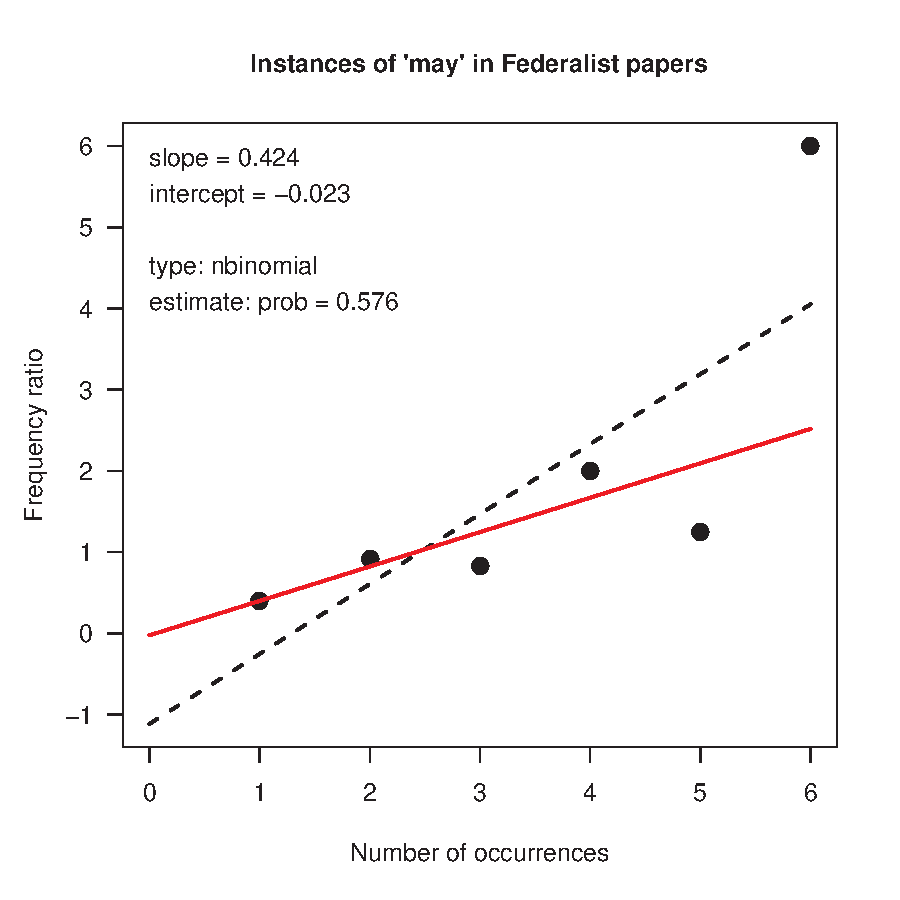
\includegraphics[width=.48\textwidth]{ch03/fig/ordplot3plot-1} 
\includegraphics[width=.48\textwidth]{ch03/fig/ordplot3plot-2} }

\caption[Ord plots for the Federalist (left) and WomenQueue (right) data sets]{Ord plots for the Federalist (left) and WomenQueue (right) data sets.\label{fig:ordplot3plot}}
\end{figure}


\end{knitrout}

\begin{Example}[queues]{Women in queues}
\citet{JinkinsonSlater:81,HoaglinTukey:85}
give the frequency distribution of the number of females observed in 100
queues of length 10 in a London Underground station, recorded
in the data set \data{WomenQueue} in \pkg{vcd}.
\begin{knitrout}
\definecolor{shadecolor}{rgb}{1, 0.961, 0.933}\color{fgcolor}\begin{kframe}
\begin{alltt}
\hlstd{> }\hlkwd{data}\hlstd{(WomenQueue,} \hlkwc{package} \hlstd{=} \hlstr{"vcd"}\hlstd{)}
\hlstd{> }\hlstd{WomenQueue}
\end{alltt}
\begin{verbatim}
nWomen
 0  1  2  3  4  5  6  7  8  9 10 
 1  3  4 23 25 19 18  5  1  1  0 
\end{verbatim}
\end{kframe}
\end{knitrout}

If it is assumed that people line up independently, and that
men and women are equally likely to be found in a queue
(not necessarily reasonable assumptions),
then the number of women out of 10
would have a (symmetric) binomial distribution with parameters $n=10$ and
$p=\frac12$.
However, there is no real reason to expect that males and females are
equally likely to be found in queues in the London underground,
so we may be interested in estimating $p$ from the data
and determining if a binomial distribution fits.
\ix{binomial distribution}

\begin{knitrout}
\definecolor{shadecolor}{rgb}{1, 0.961, 0.933}\color{fgcolor}\begin{kframe}
\begin{alltt}
\hlstd{> }\hlkwd{Ord_plot}\hlstd{(WomenQueue,} \hlkwc{main} \hlstd{=} \hlstr{"Women in queues of length 10"}\hlstd{,}
\hlstd{+ }         \hlkwc{gp} \hlstd{=} \hlkwd{gpar}\hlstd{(}\hlkwc{cex} \hlstd{=} \hlnum{1}\hlstd{),} \hlkwc{pch} \hlstd{=} \hlnum{16}\hlstd{)}
\end{alltt}
\end{kframe}
\end{knitrout}
\figref{fig:ordplot3} (right) shows the Ord plot for these data.
The negative slope and positive intercept clearly diagnose this distribution
as binomial.  The rough estimate of $\hat{p} = b/(1-b) = 0.53$ indicates that
women are slightly more prevalent than men in these data for the London
underground.
\end{Example}

\subsubsection{Limitations of Ord plots}
Using a single simple diagnostic plot to determine one of four common discrete
distributions is advantageous, but your enthusiasm should be
dampened by several weaknesses:

\begin{itemize*}
\item The Ord plot lacks resistance, since a single discrepant
       frequency affects the points $n_k / n_{k-1}$
       for both \(k\) and \(k  +  1\).

\item The sampling variance of \(k \,  n_k /  n_{k-1}\) fluctuates
       widely
       \citep{HoaglinTukey:85,JinkinsonSlater:81}.
       The use of weights \(w_k\) helps, but is purely a
       heuristic device. The \func{Ord\_plot} function explicitly shows both
       the OLS line and the WLS line, which provides some indication of the
       effect of the points on the estimation of slope and intercept.
\end{itemize*}


\ix{Ord plot|)}


\section{Poissonness plots and generalized distribution plots}\label{sec:discrete-Poissonness}

\ix{Poissonness plot|(}

The \term{Poissonness plot}
\citep{Hoaglin:80}
is a robust plot to sensitively determine how well a
one-way table of frequencies follows a \IX{Poisson distribution}.
It plots a quantity called a count metameter
against \(k\), designed
so that the result will be points along a
straight line when the data follow a \IX{Poisson distribution}.  When the
data deviate from a Poisson, the points will be curved.
\citet{HoaglinTukey:85}
develop similar plots for other discrete distributions,
including the binomial, negative binomial, and logarithmic series
distributions.  We first describe the features and construction
of these plots for the Poisson distribution and then (\secref{sec:discrete-other})
the extension to other distributions.


\ix{binomial distribution}
\ix{negative binomial distribution}

\subsection{Features of the Poissonness plot}
The Poissonness plot has the following desirable features:
\begin{itemize}
\item \boldital{Resistance}: a single discrepant value of \(n_k\)
       affects only the point at value \(k\).  (In the Ord plot
       it affects each of its neighbors.)
\item \boldital{Comparison standard}:  An approximate confidence
       interval can be found for each point, indicating its inherent
       variability and helping to judge whether each point is
       discrepant.
\item \boldital{Influence}:  Extensions of the method result in
       plots which show the effect of each point on the estimate of
       the main parameter of the distribution (\(\lambda\) in the
       Poisson).
\end{itemize}

\subsection{Plot construction}
Assume, for some fixed \(\lambda\), each observed frequency, \(n_k\)
equals the expected frequency, \(m_k = N p_k\).  Then, setting
\(n_k = N p_k  = N { e^{ - \lambda } \:  \lambda^k } /  { k ! }\),
and taking logs of both sides gives
\begin{equation*}
  \log ( n_k ) = \log \,  N - \lambda  +  k \,  \log \,  \lambda  -
  \log \,  k !
  \period
\end{equation*}
This can be rearranged to a linear equation in $k$,
\begin{equation} \label{eq:poispl}
  \phi \,  ( n_k ) \equiv \log \left(  \frac{ k ! \:  n_k } {N} \right)
 = - \lambda  +  ( \log \,  \lambda ) \,  k
 \period
\end{equation}
The left side of \eqref{eq:poispl} is called the \term{count metameter}, and
denoted \(\phi \,  ( n_k )\).  Hence,
plotting \(\phi ( n_k )\) against \(k\) should give a straight line of the form
\(\phi ( n_k )= a + b k\) with
\begin{itemize*}
\item slope = \(\log  \,  \lambda\)
\item intercept = \(- \lambda\)
\end{itemize*}
when the observed frequencies follow a Poisson distribution.
If the points in this plot are close enough to a straight line,
then an estimate of $\lambda$ may be obtained from the slope $b$ of the line,
$\hat{\lambda} = e^b$ should be reasonably close in value
to the MLE of $\lambda$, $\hat{\lambda} = \bar{x}$.
In this case, we might as well use the MLE as our estimate.

\subsubsection{Leveled plot}
If we have a preliminary estimate $\lambda_0$ of $\lambda$,
we can use this to give a new plot where the reference line
is horizontal, making comparison of the points with the line
easier.
In this leveled plot the vertical coordinate $\phi (n_k)$ is modified to
\begin{equation}\label{eq:pois-leveled}
 \phi ' (n_k) = \phi (n_k) + \lambda_0 - k \log \lambda_0
 \period
\end{equation}
When the data follow a Poisson distribution with parameter
$\lambda$, the modified plot will have
\begin{itemize*}
\item slope = \(\log  \lambda - \log  \lambda_0 = \log ( \lambda / \lambda_0 ) \)
\item intercept = \(\lambda_0 - \lambda\)
\end{itemize*}
In the ideal case, where our estimate of $\lambda_0$ is close to the true
$\lambda$, the line will be approximately
horizontal at $\phi(n_k) ' = 0$.
The modified plot is particularly useful in conjunction with the
confidence intervals for individual points described below.

\subsubsection{Confidence intervals}
The goal of the Poissonness plot is to determine whether the points
are ``sufficiently linear'' to conclude that the Poisson distribution
is adequate for the data. Confidence intervals for the points can help
you decide, and also show the relative precision of the points in these
plots.

For example, when one or two points deviate from an otherwise nearly linear
relation,
it is helpful to determine whether the discrepancy is consistent with
chance variation.
As well, we must recognize that classes with small frequencies $n_k$
are less precise than classes with large frequencies.

\citet{HoaglinTukey:85} develop approximate confidence intervals
for $\log (m_k)$ for each point in the Poissonness plot.
These are calculated as
\begin{equation}\label{eq:poisCI}
\phi \left( n_k^{*}\right) \pm h_k
\end{equation}
where the count metameter function is calculated using a modified frequency $%
n_k^{*}$, defined as
\begin{equation*}
n_k^{*}= \left\{
\begin{array}{ll}
n_k-.8n_k-.67 & n\geq 2 \\
1/e & n=1 \\
\textrm{undefined} & n=0
\end{array}
\right.
\end{equation*}
%
and $h_k$ is the half-width of the 95\% confidence interval,
\begin{equation*}
h_k=1.96\frac{\sqrt{1-\widehat{p}_k}}{[n_k-(.25\widehat{p}_k+.47)\sqrt{n_k}%
]^{1/2}}
\end{equation*}
and $\hat{p}_k = n_k / N$.


\subsection[The distplot function]{The \func{distplot} function}
Poissonness plots (and versions for other distributions)
are produced by the function \func{distplot} in \pkg{vcd}.
As with \func{Ord\_plot}, the first argument is
either a vector of counts, a one-way table of frequencies of counts or a data frame or matrix with frequencies in the first column and the corresponding counts in the second column. Nearly all of the examples in this chapter use one-way tables of counts.

The \code{type} argument specifies the type of distribution. For \code{type = "poisson"},
specifying a value for \code{lambda} $=\lambda_0$ gives the leveled version of the
plot.

\begin{Example}[horsekick4]{Death by horse kick}
The calculations for the Poissonness plot, including confidence
intervals, are shown below for the \data{HorseKicks} data.  The
call to \func{distplot}
produces the plot in the left panel of
\figref{fig:distplot1}.

\begin{knitrout}
\definecolor{shadecolor}{rgb}{1, 0.961, 0.933}\color{fgcolor}\begin{kframe}
\begin{alltt}
\hlstd{> }\hlkwd{data}\hlstd{(}\hlstr{"HorseKicks"}\hlstd{,} \hlkwc{package}\hlstd{=}\hlstr{"vcd"}\hlstd{)}
\hlstd{> }\hlstd{dp} \hlkwb{<-} \hlkwd{distplot}\hlstd{(HorseKicks,} \hlkwc{type} \hlstd{=} \hlstr{"poisson"}\hlstd{,}
\hlstd{+ }  \hlkwc{xlab}\hlstd{=}\hlstr{"Number of deaths"}\hlstd{,} \hlkwc{main}\hlstd{=}\hlstr{"Poissonness plot: HorseKicks data"}\hlstd{)}
\hlstd{> }\hlkwd{print}\hlstd{(dp,} \hlkwc{digits}\hlstd{=}\hlnum{4}\hlstd{)}
\end{alltt}
\begin{verbatim}
  Counts Freq Metameter CI.center CI.width CI.lower CI.upper
1      0  109    -0.607   -0.6131   0.1305  -0.7436  -0.4827
2      1   65    -1.124   -1.1343   0.2069  -1.3412  -0.9274
3      2   22    -1.514   -1.5451   0.4169  -1.9620  -1.1281
4      3    3    -2.408   -2.6607   1.3176  -3.9783  -1.3431
5      4    1    -2.120   -3.1203   2.6887  -5.8089  -0.4316
\end{verbatim}
\end{kframe}
\end{knitrout}
In this plot, the open circles show the calculated
observed values of the count \code{Metameter} = $\phi \,  ( n_k )$.
The smaller filled points show the centers of the confidence intervals,
\code{CI.center} = $\phi \left( n_k^{*}\right)$ (\eqref{eq:poisCI}),
and the dashed lines show the extent of the confidence intervals.

The fitted least squares line has a slope of -0.431, which would
indicate $\lambda = e^{-0.431} = 0.65$.  This compares well with the MLE,
$\lambda = \bar{x} = 0.61$.
\ixd{death by horse kick}

Using \code{lambda = 0.61} as below gives the leveled version shown in
the right panel of \figref{fig:distplot1}.
\begin{knitrout}
\definecolor{shadecolor}{rgb}{1, 0.961, 0.933}\color{fgcolor}\begin{kframe}
\begin{alltt}
\hlstd{> }\hlcom{# leveled version, specifying lambda}
\hlstd{> }\hlkwd{distplot}\hlstd{(HorseKicks,} \hlkwc{type} \hlstd{=} \hlstr{"poisson"}\hlstd{,} \hlkwc{lambda} \hlstd{=} \hlnum{0.61}\hlstd{,}
\hlstd{+ }  \hlkwc{xlab}\hlstd{=}\hlstr{"Number of deaths"}\hlstd{,} \hlkwc{main}\hlstd{=}\hlstr{"Leveled Poissonness plot"}\hlstd{)}
\end{alltt}
\end{kframe}
\end{knitrout}

\begin{figure}[htbp]
\centerline{
\includegraphics[width=.48\textwidth]{ch03/fig/distplot1}
\includegraphics[width=.48\textwidth]{ch03/fig/distplot2}
}
\caption[Poissonness plots for the HorseKick data]{Poissonness plots for the HorseKick data. Left: standard plot; right: leveled plot.\label{fig:distplot1}}
\end{figure}

\TODO{DM: In the leveled plot, the label for the slope is actually
  wrong, should be exp(slope + log $\lambda$) = 0.65}

In both plots the fitted line is within the confidence intervals,
indicating the adequacy of the Poisson model for these data.
The widths of the intervals for $k > 2$ are graphic reminders that these observations
have decreasingly low precision where the counts $n_k$ are small.

\end{Example}

% \subsection{Leverage and influence}
% \TODO{This subsection should be omitted, unless we extend the calculation and plotting
% methods.}

\ix{Poissonness plot|)}

\subsection{Plots for other distributions}\label{sec:discrete-other}
As described in \secref{sec:pwrseries}, the binomial, Poisson, negative binomial,
geometric, and logseries distributions are all members of the
general  power series family of discrete distributions.
For this family, \citet{HoaglinTukey:85} develop similar plots
of a count metameter against $k$ which appear as a straight line
when a data distribution follows a given family member.

The distributions which can be analyzed in this way are shown in
\tabref{tab:distparms}, with the interpretation given to the
slope and intercept in each case.
For example, for the Binomial distribution, a ``binomialness''
plot is constructed by plotting $\log n_k^{*} / N \binom{n}{k}$
against $k$.  If the points in this plot approximate a straight
line, the slope is interpreted as $\log (p/(1-p))$, so the
binomial parameter $p$ may be estimated as $p = e^b/(1+e^b)$.
\begin{table}[!b]
\caption[Plot parameters for five discrete distributions]{Plot parameters for five discrete distributions. In each case the count metameter, $\phi
(n_k^{*})$ is plotted against $k$, yielding a straight line when the data
follow the given distribution.}
\label{tab:distparms}
 \begin{center}
\begin{tabular}{p{2.4cm}llll}
  \hline
  \tableheader
%              & Probability      & Count                      & Theoretical & Theoretical \\
%Distributiion & function, $p(k)$ & metameter, $\phi(n_k^{*})$ & Slope ($b$) & Intercept ($a$)\\[1ex]
  \multilineL{Distribution\\} & \multilineL{Probability\\function, $p(k)$} & \multilineL{Count)\\metameter, $\phi(n_k^{*})$} & \multilineL{Theoretical\\ slope ($b$)} &
  \multilineL{Theoretical\\ intercept ($a$)} \\
  \hline \\[.3ex]
Poisson          & $e^{-\lambda }\lambda ^k/k!$ & $\log (k!n_k^{*}/N)$ & $\log
(\lambda )$ & -$\lambda $ \\[.7ex]
%
Binomial          & $\binom nkp^k(1-p)^{n-k}$ & $\log \left( n_k^{*}/N\binom
nk\right) $ & $\log \left(\frac{p}{1-p}\right)$ & $n\log (1-p)$ \\[.7ex]
%
Negative binomial & $\binom{n+k-1}kp^n(1-p)^k$ & $\log \left( n_k^{*}/N%
\binom{n+k-1}k\right) $ & $\log (1-p)$ & $n\log (p)$ \\[.7ex]
%
Geometric         & $p(1-p)^k$ & $\log \left( n_k^{*}/N\right) $ & $\log (1-p)$ & $\log (p)$ \\[.7ex]
%
Log series        & $\theta ^k/[-k\log (1-\theta )]$ & $\log \left(
kn_k^{*}/N\right) $ & $\log (\theta )$ & $-\log \left( -\log (1-\theta)\right) $ \\[1ex]%
  \hline
  \multicolumn{5}{p{\textwidth}}{\emph{Source}: adapted from \citet{HoaglinTukey:85}, Table 9-15.} \\
\end{tabular}
 \end{center}
\end{table}



Unlike the Ord plot, a different plot is required for each distribution,
because the count metameter, \(\phi ( n_k )\), differs
from distribution to distribution.
Moreover, systematic deviation from a linear relationship does not
       indicate which distribution provides a better fit.
However, the attention to robustness, and the availability of confidence
intervals and influence diagnostics make this a highly useful tool
for visualizing discrete distributions.

\begin{Example}[saxony-distplot]{Families in Saxony}
Our analysis in \exref{ex:saxony1} and \exref{ex:saxfit} of
the \data{Saxony} data
showed that the distribution of male children had slightly heavier tails
than the binomial, meaning the observed distribution is overdispersed.
We can see this in the \func{goodfit} plot shown in \figref{fig:distplot3} (left),
and even more clearly in the distribution diagnostic
plot produced
by \func{distplot} in the right panel of \figref{fig:distplot3}.
For a binomial distribution, we call
this distribution plot a ``binomialness plot''.

\begin{knitrout}
\definecolor{shadecolor}{rgb}{1, 0.961, 0.933}\color{fgcolor}\begin{kframe}
\begin{alltt}
\hlstd{> }\hlkwd{plot}\hlstd{(}\hlkwd{goodfit}\hlstd{(Saxony,} \hlkwc{type}\hlstd{=}\hlstr{"binomial"}\hlstd{,} \hlkwc{par}\hlstd{=}\hlkwd{list}\hlstd{(}\hlkwc{size}\hlstd{=}\hlnum{12}\hlstd{)))}
\hlstd{> }\hlkwd{distplot}\hlstd{(Saxony,} \hlkwc{type} \hlstd{=} \hlstr{"binomial"}\hlstd{,} \hlkwc{size} \hlstd{=} \hlnum{12}\hlstd{,}
\hlstd{+ }  \hlkwc{xlab}\hlstd{=}\hlstr{"Number of males"}\hlstd{)}
\end{alltt}
\end{kframe}\begin{figure}[!htbp]

\centerline{\includegraphics[width=.49\textwidth]{ch03/fig/distplot3-1} 
\includegraphics[width=.49\textwidth]{ch03/fig/distplot3-2} }

\caption{Diagnostic plots for males in Saxony families. Left: \func{goodfit} plot; right: \func{distplot} plot. Both plots show heavier tails than in a binomial distribution.\label{fig:distplot3}}
\end{figure}


\end{knitrout}
The weight of evidence is thus that, as simple as the binomial might be,
it is inadequate to fully explain the distribution of sex ratios in this
large sample of families of 12 children.
To understand this data better, it is necessary to question the assumptions
of the binomial (births of males are independent
Bernoulli trials with constant probability $p$)
as a model for this birth distribution and/or find a more
adequate model.%
\footnote{
On these questions, \citet{Edwards:1958} reviews
numerous other studies of these Geissler's data, and fits a so-called
\term{$\beta$-binomial} model proposed by \citet{Skellam:1948},
where $p$ varies among families according to a $\beta$ distribution.
He concludes that there
is evidence that $p$ varies between families of the same size.  One suggested
explanation is that family decisions to have a further child is influenced by
the balance of boys and girls among their earlier children.
}
\end{Example}


\begin{Example}[federalist-distplot]{Federalist papers}
In \exref{ex:Fedfit} we carried out GOF tests for the Poisson and
negative binomial models with the Federalist papers data;
\figref{fig:Fed0-Fed1} showed the corresponding rootogram plots.
\figref{fig:distplot5} compares these two using the diagnostic plots of
this section. Again the Poisson shows systematic departure from the
linear relation required in the Poissonness plot, while the
negative binomial model provides an acceptable fit to
these data.
\begin{knitrout}
\definecolor{shadecolor}{rgb}{1, 0.961, 0.933}\color{fgcolor}\begin{kframe}
\begin{alltt}
\hlstd{> }\hlkwd{distplot}\hlstd{(Federalist,} \hlkwc{type} \hlstd{=} \hlstr{"poisson"}\hlstd{,} \hlkwc{xlab}\hlstd{=}\hlstr{"Occurrences of 'may'"}\hlstd{)}
\hlstd{> }\hlkwd{distplot}\hlstd{(Federalist,} \hlkwc{type} \hlstd{=} \hlstr{"nbinomial"}\hlstd{,} \hlkwc{xlab}\hlstd{=}\hlstr{"Occurrences of 'may'"}\hlstd{)}
\end{alltt}
\end{kframe}\begin{figure}[!htbp]

\centerline{\includegraphics[width=.49\textwidth]{ch03/fig/distplot5-1} 
\includegraphics[width=.49\textwidth]{ch03/fig/distplot5-2} }

\caption[Diagnostic plots for the Federalist papers data]{Diagnostic plots for the Federalist papers data. Left: Poissonness plot; right: negative binomialness plot.\label{fig:distplot5}}
\end{figure}


\end{knitrout}
\end{Example}

\TODO{DM: The following section assumes knowledge of GLMs, introduced in a
later chapter. Either remove chapter, or move to the end after the GLM
chapter.}

\section{Fitting discrete distributions as generalized linear models}\label{sec:fitglm}

In \secref{sec:pwrseries}, we described how the common discrete distributions
are all members of the general power series family.  This provides the
basis for the generalized distribution plots described in \secref{sec:discrete-other}.
Another general family of distributions---the \term{exponential family}---%
includes most of the common continuous distributions:
the normal, gamma, exponential, and others,
and is the basis of the class of generalized linear models (GLMs) fit
by \func{glm}.

A clever approach by
\citet{LindseyMersch:92}, \citet[\S 6.1]{Lindsey:95} shows how various discrete
(and continuous)
distributions can be fit to frequency data using generalized linear models
for log frequency (which are equivalent to Poisson \loglin models).
The uniform, geometric, binomial, and the
Poisson distributions may all be fit easily in this way, but the idea extends
to some other distributions, such as the \term{double binomial} distribution,
that allows a separate parameter for overdispersion relative to the binomial.
A clear advantage is that this method gives estimated standard errors for the
distribution parameters as well as estimated confidence intervals
for fitted probabilities.

The essential idea is that, for frequency data, any distribution in the
exponential family may be represented by a linear model for the logarithm
of the cell frequency, with a Poisson distribution for errors,
otherwise known as a ``Poisson \loglin\ regression model''.
These have the form
\begin{equation*}
\log (N \pi_k) = \textrm{ offset } + \beta_0 + \vec{\beta}\trans \vec{S}(k)
 \comma
\end{equation*}
where $N$ is the total frequency, $\pi_k$ is the modeled probability
of count $k$,
$\vec{S}(k)$ is a vector of zero or more sufficient statistics for the
canonical parameters of the exponential family distribution,
and the offset term is a value which does not depend on the
parameters.

\tabref{tab:expfamily} shows the sufficient statistics and
offsets for several discrete distributions.
See \citet{LindseyMersch:92} for further details, and definitions
for the double-binomial distribution,%
\footnote{
In \R, the double binomial distribution is implemented in the
\Rpackage{rmutil}, providing the standard complement of
density function (\func{ddoublebinom}), CDF (\func{pdoublebinom}),
quantiles (\func{qdoublebinom})
and random generation (\func{rdoublebinom}).
}
and \citet[pp. 130--133]{Lindsey:95}
for his analysis of the \data{Saxony} data using this distribution.
\citet{LindseyAltham:1998} provide an analysis of the
complete Geissler data (provided in the data set \data{Geissler} in \pkg{vcdExtra})
using several different models to
handle overdispersion.
\begin{table}[tb]
 \caption{Poisson \loglin\ representations for some discrete distributions}\label{tab:expfamily}
 \begin{center}
{\renewcommand{\arraystretch}{1.2}
 \begin{tabular}{lll}
  \hline
  Distribution & Sufficient statistics & Offset \\
  \hline
  Geometric & $k$ \\
  Poisson & $k$ & $-\log(k!)$ \\
  Binomial & $k$ & $\log{\binom{n}{k}}$ \\
  Double binomial & $k, k \log(k) + (n-k) \log(n-k)$ & $\log{\binom{n}{k}}$ \\
  \hline
 \end{tabular}
}
 \end{center}
\end{table}


\begin{Example}[saxony2]{Families in Saxony}
The binomial distribution and the double binomial can both be fit to frequency data as a Poisson regression via \func{glm}
using $\log \binom{n}{k}$ as an offset.
First, we convert \data{Saxony} into a numeric data frame for use with \func{glm}.
\begin{knitrout}
\definecolor{shadecolor}{rgb}{1, 0.961, 0.933}\color{fgcolor}\begin{kframe}
\begin{alltt}
\hlstd{> }\hlkwd{data}\hlstd{(Saxony,} \hlkwc{package}\hlstd{=}\hlstr{"vcd"}\hlstd{)}
\hlstd{> }\hlstd{Males} \hlkwb{<-} \hlkwd{as.numeric}\hlstd{(}\hlkwd{names}\hlstd{(Saxony))}
\hlstd{> }\hlstd{Families} \hlkwb{<-} \hlkwd{as.vector}\hlstd{(Saxony)}
\hlstd{> }\hlstd{Sax.df} \hlkwb{<-} \hlkwd{data.frame}\hlstd{(Males, Families)}
\end{alltt}
\end{kframe}
\end{knitrout}
To calculate the offset  for \func{glm} in \R,
note that \code{choose(12,0:12)} returns the
binomial coefficients, and \code{lchoose(12,0:12)} returns their logs.
\begin{knitrout}
\definecolor{shadecolor}{rgb}{1, 0.961, 0.933}\color{fgcolor}\begin{kframe}
\begin{alltt}
\hlstd{> }\hlcom{# fit binomial (12, p) as a glm}
\hlstd{> }\hlstd{Sax.bin} \hlkwb{<-} \hlkwd{glm}\hlstd{(Families} \hlopt{~} \hlstd{Males,} \hlkwc{offset}\hlstd{=}\hlkwd{lchoose}\hlstd{(}\hlnum{12}\hlstd{,}\hlnum{0}\hlopt{:}\hlnum{12}\hlstd{),}
\hlstd{+ }               \hlkwc{family}\hlstd{=poisson,} \hlkwc{data}\hlstd{=Sax.df)}
\hlstd{> }
\hlstd{> }\hlcom{# brief model summaries}
\hlstd{> }\hlkwd{LRstats}\hlstd{(Sax.bin)}
\end{alltt}
\begin{verbatim}
Likelihood summary table:
        AIC BIC LR Chisq Df Pr(>Chisq)    
Sax.bin 191 192       97 11      7e-16 ***
---
Signif. codes:  0 '***' 0.001 '**' 0.01 '*' 0.05 '.' 0.1 ' ' 1
\end{verbatim}
\begin{alltt}
\hlstd{> }\hlkwd{coef}\hlstd{(Sax.bin)}
\end{alltt}
\begin{verbatim}
(Intercept)       Males 
  -0.069522    0.076898 
\end{verbatim}
\end{kframe}
\end{knitrout}
As we have seen, this model fits badly.
The parameter estimate for \texttt{Males}, $\beta_1 = 0.0769$
is actually estimating the logit of $p$, $\log p / (1-p)$,
so the inverse transformation gives
$\hat{p} = \frac{\exp (\beta_1)}{1 + \exp (\beta_1)} = 0.5192$,
as we had before.


The double binomial model can be fitted as follows.
The term \code{YlogitY} calculates
$k \log(k) + (n-k) \log(n-k)$,
%$-k \log(\frac{k}{n-k})$,
the second sufficient statistic for the double binomial
(see \tabref{tab:expfamily})
fitted via \func{glm}.
%\DONE{Fixed \tabref{tab:expfamily} entry here}

\begin{knitrout}
\definecolor{shadecolor}{rgb}{1, 0.961, 0.933}\color{fgcolor}\begin{kframe}
\begin{alltt}
\hlstd{> }\hlcom{# double binomial, (12, p, psi)}
\hlstd{> }\hlstd{Sax.df}\hlopt{$}\hlstd{YlogitY} \hlkwb{<-}
\hlstd{+ }  \hlstd{Males}      \hlopt{*} \hlkwd{log}\hlstd{(}\hlkwd{ifelse}\hlstd{(Males}\hlopt{==}\hlnum{0}\hlstd{,} \hlnum{1}\hlstd{, Males))} \hlopt{+}
\hlstd{+ }        \hlstd{(}\hlnum{12}\hlopt{-}\hlstd{Males)} \hlopt{*} \hlkwd{log}\hlstd{(}\hlkwd{ifelse}\hlstd{(}\hlnum{12}\hlopt{-}\hlstd{Males}\hlopt{==}\hlnum{0}\hlstd{,} \hlnum{1}\hlstd{,} \hlnum{12}\hlopt{-}\hlstd{Males))}
\hlstd{> }
\hlstd{> }\hlstd{Sax.dbin} \hlkwb{<-} \hlkwd{glm}\hlstd{(Families} \hlopt{~} \hlstd{Males} \hlopt{+} \hlstd{YlogitY,} \hlkwc{offset}\hlstd{=}\hlkwd{lchoose}\hlstd{(}\hlnum{12}\hlstd{,}\hlnum{0}\hlopt{:}\hlnum{12}\hlstd{),}
\hlstd{+ }        \hlkwc{family}\hlstd{=poisson,} \hlkwc{data}\hlstd{=Sax.df)}
\hlstd{> }\hlkwd{coef}\hlstd{(Sax.dbin)}
\end{alltt}
\begin{verbatim}
(Intercept)       Males     YlogitY 
  -3.096918    0.065977    0.140205 
\end{verbatim}
\begin{alltt}
\hlstd{> }\hlkwd{LRstats}\hlstd{(Sax.bin, Sax.dbin)}
\end{alltt}
\begin{verbatim}
Likelihood summary table:
         AIC BIC LR Chisq Df Pr(>Chisq)    
Sax.bin  191 192     97.0 11      7e-16 ***
Sax.dbin 109 111     13.1 10       0.22    
---
Signif. codes:  0 '***' 0.001 '**' 0.01 '*' 0.05 '.' 0.1 ' ' 1
\end{verbatim}
\end{kframe}
\end{knitrout}
From the above, we can see that
the double binomial model \code{Sax.dbin} with one more parameter
is significantly better than the simple binomial
and represents an adequate fit to the data.  The table below
displays the fitted values and standardized residuals for both models.
\begin{knitrout}
\definecolor{shadecolor}{rgb}{1, 0.961, 0.933}\color{fgcolor}\begin{kframe}
\begin{alltt}
\hlstd{> }\hlstd{results} \hlkwb{<-} \hlkwd{data.frame}\hlstd{(Sax.df,}
\hlstd{+ }          \hlkwc{fit.bin}\hlstd{=}\hlkwd{fitted}\hlstd{(Sax.bin),} \hlkwc{res.bin}\hlstd{=}\hlkwd{rstandard}\hlstd{(Sax.bin),}
\hlstd{+ }          \hlkwc{fit.dbin}\hlstd{=}\hlkwd{fitted}\hlstd{(Sax.dbin),} \hlkwc{res.dbin}\hlstd{=}\hlkwd{rstandard}\hlstd{(Sax.dbin))}
\hlstd{> }\hlkwd{print}\hlstd{(results,} \hlkwc{digits}\hlstd{=}\hlnum{2}\hlstd{)}
\end{alltt}
\begin{verbatim}
   Males Families YlogitY fit.bin res.bin fit.dbin res.dbin
1      0        3      30    0.93    1.70      3.0    0.026
2      1       24      26   12.09    3.05     23.4    0.136
3      2      104      24   71.80    3.71    104.3   -0.036
4      3      286      23  258.48    1.87    307.8   -1.492
5      4      670      22  628.06    1.94    652.9    0.778
6      5     1033      22 1085.21   -1.87   1038.5   -0.202
7      6     1343      22 1367.28   -0.75   1264.2    2.635
8      7     1112      22 1265.63   -5.09   1185.0   -2.550
9      8      829      22  854.25   -1.03    850.1   -0.846
10     9      478      23  410.01    3.75    457.2    1.144
11    10      181      24  132.84    4.23    176.8    0.371
12    11       45      26   26.08    3.42     45.2   -0.039
13    12        7      30    2.35    2.45      6.5    0.192
\end{verbatim}
\end{kframe}
\end{knitrout}
Finally, \figref{fig:sax-glm5} shows the rootogram for the double
binomial, which can be compared with that for the binomial model
shown in \figref{fig:distplot3}.  We can see that the fit is now
quite good, particularly in the tails.  The positive coefficient
for the term \code{YlogitY} gives additional weight in the tails.
\begin{knitrout}
\definecolor{shadecolor}{rgb}{1, 0.961, 0.933}\color{fgcolor}\begin{kframe}
\begin{alltt}
\hlstd{> }\hlkwd{with}\hlstd{(results, vcd}\hlopt{::}\hlkwd{rootogram}\hlstd{(Families, fit.dbin,}
\hlstd{+ }                        \hlkwc{xlab}\hlstd{=}\hlstr{"Number of males"}\hlstd{))}
\end{alltt}
\end{kframe}\begin{figure}[!htbp]

\centerline{\includegraphics[width=.6\textwidth]{ch03/fig/sax-glm5-1} }

\caption[Rootogram for the double binomial model for the Saxony data]{Rootogram for the double binomial model for the Saxony data. This now fits well in the tails of the distribution.\label{fig:sax-glm5}}
\end{figure}


\end{knitrout}


%\TODO{Interpret the coefficient for YlogitY in terms of dispersion??}

\end{Example}

\subsection{Covariates, overdispersion and excess zeros}
All of the examples in this chapter are somewhat special, in that in each case the
data consist only of a one-way frequency distribution of a basic count variable.
In more general and realistic settings, there may also be one or more explanatory
variables or \term{covariate}s that influence the frequency distributions of the
counts.  For example, in the \data{Saxony} data, the number of boys in families
of size 12 was aggregated over the years 1876--1885, and it is possible that
any deviation from a binomial distribution could be due to variation over time
or unmeasured predictors (e.g., rural vs.\ urban, age of parents).

This is where the generalized linear model
approach introduced here (treated in detail in \chref{ch:glm}),
begins to shine--- because it
allows such covariates to be taken into account, and then questions regarding
the \emph{form} of the distribution pertain only to the variation of the
frequencies not fitted by the model.  The next example illustrates what
can go wrong when important predictors are omitted from the analysis.

\begin{Example}[phdpubs0]{Publications of PhD candidates}
\citet{Long:1990,Long:1997} gave data on the number of publications by 915 doctoral candidates in biochemistry
in the last three years of their PhD studies, contained in the
data set \data{PhdPubs} in \pkg{vcdExtra}.  The data set also includes information
on gender, marital status, number of young children, prestige of the doctoral department
and number of publications by the student's mentor.
The frequency distribution of number of publications by these students is shown below.

\begin{knitrout}
\definecolor{shadecolor}{rgb}{1, 0.961, 0.933}\color{fgcolor}\begin{kframe}
\begin{alltt}
\hlstd{> }\hlkwd{data}\hlstd{(}\hlstr{"PhdPubs"}\hlstd{,} \hlkwc{package}\hlstd{=}\hlstr{"vcdExtra"}\hlstd{)}
\hlstd{> }\hlkwd{table}\hlstd{(PhdPubs}\hlopt{$}\hlstd{articles)}
\end{alltt}
\begin{verbatim}

  0   1   2   3   4   5   6   7   8   9  10  11  12  16  19 
275 246 178  84  67  27  17  12   1   2   1   1   2   1   1 
\end{verbatim}
\end{kframe}
\end{knitrout}
The naive approach, ignoring the potential predictors is just to try fitting various
probability models to this one-way distribution. Rootograms for the simpler
Poisson distribution and the negative binomial that allows for overdispersion are
shown in \figref{fig:phdpubs-rootogram}.

\begin{knitrout}
\definecolor{shadecolor}{rgb}{1, 0.961, 0.933}\color{fgcolor}\begin{kframe}
\begin{alltt}
\hlstd{> }\hlkwd{library}\hlstd{(vcd)}
\hlstd{> }\hlkwd{plot}\hlstd{(}\hlkwd{goodfit}\hlstd{(PhdPubs}\hlopt{$}\hlstd{articles),} \hlkwc{xlab}\hlstd{=}\hlstr{"Number of Articles"}\hlstd{,}
\hlstd{+ }     \hlkwc{main}\hlstd{=}\hlstr{"Poisson"}\hlstd{)}
\hlstd{> }\hlkwd{plot}\hlstd{(}\hlkwd{goodfit}\hlstd{(PhdPubs}\hlopt{$}\hlstd{articles,} \hlkwc{type}\hlstd{=}\hlstr{"nbinomial"}\hlstd{),} \hlkwc{xlab}\hlstd{=}\hlstr{"Number of Articles"}\hlstd{,}
\hlstd{+ }     \hlkwc{main}\hlstd{=}\hlstr{"Negative binomial"}\hlstd{)}
\end{alltt}
\end{kframe}\begin{figure}[!htbp]

\centerline{\includegraphics[width=.48\textwidth]{ch03/fig/phdpubs-rootogram-1} 
\includegraphics[width=.48\textwidth]{ch03/fig/phdpubs-rootogram-2} }

\caption[Hanging rootograms for publications by PhD candidates, comparing the Poisson and negative binomial models]{Hanging rootograms for publications by PhD candidates, comparing the Poisson and negative binomial models. The Poisson model clearly does not fit. The the negative binomial is better, but still has significant lack of fit.\label{fig:phdpubs-rootogram}}
\end{figure}


\end{knitrout}
From these plots it is clear that the Poisson distribution doesn't fit well at all,
because there is a large excess of zero counts--- candidates with no publications,
and most of the counts of four or more publications are larger than the Poisson model
predicts.
The fit of the negative binomial model in the right panel of \figref{fig:phdpubs-rootogram}
looks much better, except that for eight or more publications, there is a
systematic tendency of overfitting for 8--10 and underfittting for the observed
counts of 12 or more. This lack of fit is confirmed by the formal test.
\begin{knitrout}
\definecolor{shadecolor}{rgb}{1, 0.961, 0.933}\color{fgcolor}\begin{kframe}
\begin{alltt}
\hlstd{> }\hlkwd{summary}\hlstd{(}\hlkwd{goodfit}\hlstd{(PhdPubs}\hlopt{$}\hlstd{articles,} \hlkwc{type}\hlstd{=}\hlstr{"nbinomial"}\hlstd{))}
\end{alltt}
\begin{verbatim}

	 Goodness-of-fit test for nbinomial distribution

                    X^2 df  P(> X^2)
Likelihood Ratio 31.098 12 0.0019033
\end{verbatim}
\end{kframe}
\end{knitrout}

The difficulty with this simple analysis is not only that it ignores the possible
predictors of publishing by these PhD candidates, but also, by doing so, it
prevents a better, more nuanced explanation of the phenomenon under study.
This example is re-visited in \chref{ch:glm},
\exref{ex:phdpubs1},
where we consider generalized linear models taking potential predictors into
account, as well as extended \emph{zero-inflated}
models allowing special consideration of zero counts.
\end{Example}

\section{Chapter summary}\label{sec:ch03-summary}

\begin{itemize}
\item Discrete distributions typically involve basic \emph{counts} of occurrences
of some event occurring with varying \emph{frequency}. The ideas and methods
for one-way tables described in this chapter are building blocks for
the analysis of more complex data.

\item The most commonly used discrete distributions include the binomial,
Poisson, negative binomial, geometric, and logarithmic series distributions.
Happily, these are all members of a family called the
power series distributions.
Methods of fitting an observed data set to any of these distributions are
described, and implemented in the \func{goodfit} function.

\item After fitting an observed distribution it is useful to plot the observed
and fitted frequencies.
Several ways of making these plots are described, and implemented in the
\func{rootogram} function.

\item A heuristic graphical method for identifying which discrete distribution is most
appropriate for a given set of data involves plotting ratios
$k n_k / n_{k-1}$ against $k$.
These plots are constructed by the function \func{Ord\_plot}.

\item A more robust plot for a Poisson distribution involves plotting
a count metameter, $\phi ( n_k ) $ against $k$, which
gives a straight line (whose slope estimates the Poisson parameter)
if the data follow a Poisson distribution.
This plot provides robust confidence intervals for individual points
and provides a means to assess the influence of individual points
on the Poisson parameter.
These plots are provided by the function \func{distplot}.

\item The ideas behind the Poissonness plot can be applied to the other
discrete distributions.
\end{itemize}


%\section{Further reading}\label{sec:ch03-reading}

\section{Lab exercises}\label{sec:ch03-labs}

\begin{Exercises}
  \exercise The \data{Arbuthnot} data in \pkg{HistData} (\exref{ex:arbuthnot1}) also
   contains the variable
   \code{Ratio}, giving the ratio of male to female births.
	  \begin{enumerate*}
	    \item Make a plot of \code{Ratio} over \code{Year}, similar to \figref{fig:arbuthnot1}.
	    What features stand out?  Which plot do you prefer to display the tendency for
	    more male births?
	    \item Plot the total number of christenings, \code{Males + Females} or \code{Total}
	    (in 000s) over time.
	    What unusual features do you see?
	  \end{enumerate*}

  \exercise Use the graphical methods illustrated in \secref{sec:discrete-distrib}
  to plot a collection of geometric distributions for $p = 0.2, 0.4, 0.6, 0.8$,
  over a range of values of $k = 0, 1, \dots 10$.
  \begin{enumerate}
    \item With \func{xyplot}, try the different plot formats using points
    connected with lines, as in \figref{fig:dbinom2-plot}, or using points
    and lines down to the origin, as in the panels of \figref{fig:dpois-xyplot1}.
    \item Also with \func{xyplot}, produce one version of a multi-line plot
    in a single panel that you think shows well how these distributions change
    with the probability $p$ of success.
    \item Do the same in a multi-panel version, conditional on $p$.
  \end{enumerate}

  \exercise Use the data set \data{WomenQueue} to:
  \begin{enumerate*}
    \item produce plots analogous to those
  shown in \secref{sec:discrete-intro} (some sort of bar graph of frequencies)
    \item check for goodness-of-fit to the binomial distribution using the
    \func{goodfit} methods described in \secref{sec:fitplot}.
  \end{enumerate*}

  \exercise Continue \exref{ex:saxfit} on the distribution of male children in families
  in Saxony by fitting a binomial distribution, $\Bin(n=12, p=\frac12)$, specifying
  equal probability for boys and girls. [Hint:  you need to specify both \code{size} and
  \code{prob} values for \func{goodfit}.]
  \begin{enumerate*}
    \item Carry out the GOF test for this fixed binomial distribution.
    What is the ratio of $\chi^2 / df$? What do you conclude?
    \item Test the additional lack of fit for the model $\Bin(n=12, p=\frac12)$
    compared to the model $\Bin(n=12, p=\hat{p})$ where $\hat{p}$ is estimated
    from the data.
    \item Use the \func{plot.gootfit} method to visualize these two models.
  \end{enumerate*}

  \exercise For the \data{Federalist} data, the examples in \secref{sec:fitdistr} and
  \secref{sec:fitplot} showed the negative binomial to provide an acceptable fit.
  Compare this with the simpler special case of geometric distribution, corresponding
  to $n=1$.
  \begin{enumerate*}
    \item Use \func{goodfit} to fit the geometric distribution. [Hint: use \code{type="nbinomial"}, but specify \code{size=1} as a parameter.]
    \item Compare the negative binomial and the geometric models statistically,
    by a \LR test of the difference between these two models.
    \item Compare the negative binomial and the geometric models visually
    by hanging rootograms or other methods.
  \end{enumerate*}

  \exercise \citet[Table 2.4]{MostellerWallace:63} give the frequencies, $n_k$
  of counts $k = 0, 1, \dots$ of other selected marker words in 247 blocks
  of text known to have been written by Alexander Hamilton.  The data below
  show the occurrences of the word \emph{upon}, that Hamilton used much more than
  did James Madison.
\begin{knitrout}
\definecolor{shadecolor}{rgb}{1, 0.961, 0.933}\color{fgcolor}\begin{kframe}
\begin{alltt}
\hlstd{> }\hlstd{count} \hlkwb{<-} \hlnum{0} \hlopt{:} \hlnum{5}
\hlstd{> }\hlstd{Freq} \hlkwb{<-} \hlkwd{c}\hlstd{(}\hlnum{129}\hlstd{,} \hlnum{83}\hlstd{,} \hlnum{20}\hlstd{,} \hlnum{9}\hlstd{,} \hlnum{5}\hlstd{,} \hlnum{1}\hlstd{)}
\end{alltt}
\end{kframe}
\end{knitrout}
  \begin{enumerate*}
    \item Read these data into \R and construct a one-way table of frequencies of counts
    or a matrix or data frame with frequencies in the first column and the corresponding counts in the second column, suitable for use with \func{goodfit}.
    \item Fit and plot the Poisson model for these frequencies.
    \item Fit and plot the negative binomial model for these frequencies.
    \item What do you conclude?
  \end{enumerate*}

  \exercise The data frame \data{Geissler} in the \Rpackage{vcdExtra} contains the complete data from Geissler's \citeyearpar{Geissler:1889} tabulation of family sex composition in Saxony.  The table below gives the number of boys in families of size 11.

% latex table generated in R 3.0.1 by xtable 1.7-2 package
% Tue Dec 17 10:15:54 2013
%\begin{table}[ht]
%\centering
\begin{tabular}{rrrrrrrrrrrrr}
%  \hline
% & 1 & 2 & 3 & 4 & 5 & 6 & 7 & 8 & 9 & 10 & 11 & 12 \\
  \hline
boys &   0 &   1 &   2 &   3 &   4 &   5 &   6 &   7 &   8 &   9 &  10 &  11 \\
  Freq &   8 &  72 & 275 & 837 & 1,540 & 2,161 & 2,310 & 1,801 & 1,077 & 492 &  93 &  24 \\
   \hline
\end{tabular}
%\end{table}
% the table is better

  \begin{enumerate*}
    \item Read these data into \R
    \item Following \exref{ex:saxfit}, use \func{goodfit} to fit the binomial model and plot the
    results.  Is there an indication that the binomial does not fit these data?
    \item Diagnose the form of the distribution using the methods described in \secref{sec:discrete-ord}.
    \item Try fitting the negative binomial distribution, and use \func{distplot} to diagnose
    whether the negative binomial is a reasonable fit.
  \end{enumerate*}

  \exercise The data frame \data{Bundesliga} gives a similar data set to that for UK soccer scores
  (\data{UKSoccer})
  examined in \exref{ex:soccer}, but over a wide range of years.  The following lines calculate
  a two-way table, \code{BL1995}, of home-team and away-team goals
  for the 306 games in the year 1995.
\begin{knitrout}
\definecolor{shadecolor}{rgb}{1, 0.961, 0.933}\color{fgcolor}\begin{kframe}
\begin{alltt}
\hlstd{> }\hlkwd{data}\hlstd{(}\hlstr{"Bundesliga"}\hlstd{,} \hlkwc{package} \hlstd{=} \hlstr{"vcd"}\hlstd{)}
\hlstd{> }\hlstd{BL1995} \hlkwb{<-} \hlkwd{xtabs}\hlstd{(}\hlopt{~} \hlstd{HomeGoals} \hlopt{+} \hlstd{AwayGoals,} \hlkwc{data} \hlstd{= Bundesliga,}
\hlstd{+ }                \hlkwc{subset} \hlstd{= (Year} \hlopt{==} \hlnum{1995}\hlstd{))}
\hlstd{> }\hlstd{BL1995}
\end{alltt}
\begin{verbatim}
         AwayGoals
HomeGoals  0  1  2  3  4  5  6
        0 26 16 13  5  0  1  0
        1 19 58 20  5  4  0  1
        2 27 23 20  5  1  1  1
        3 14 11 10  4  2  0  0
        4  3  5  3  0  0  0  0
        5  4  1  0  1  0  0  0
        6  1  0  0  1  0  0  0
\end{verbatim}
\end{kframe}
\end{knitrout}
  \begin{enumerate*}
    \item As in \exref{ex:soccer}, find the one-way distributions of \code{HomeGoals},
    \code{AwayGoals} and \code{TotalGoals = HomeGoals + AwayGoals}.
    \item Use \func{goodfit} to fit and plot the Poisson distribution to each of these.  Does the
    Poisson seem to provide a reasonable fit?
    \item Use \func{distplot} to assess fit of the Poisson distribution.
    \item What circumstances of scoring goals in soccer might cause these distributions to
    deviate from Poisson distributions?
  \end{enumerate*}

  \item\hard
  Repeat the exercise above, this time using the data for all years in which there was
  the standard number (306) of games, that is for \code{Year>1965}, tabulated as shown below.
\begin{knitrout}
\definecolor{shadecolor}{rgb}{1, 0.961, 0.933}\color{fgcolor}\begin{kframe}
\begin{alltt}
\hlstd{> }\hlstd{BL} \hlkwb{<-} \hlkwd{xtabs}\hlstd{(}\hlopt{~} \hlstd{HomeGoals} \hlopt{+} \hlstd{AwayGoals,} \hlkwc{data} \hlstd{= Bundesliga,}
\hlstd{+ }            \hlkwc{subset} \hlstd{= (Year} \hlopt{>} \hlnum{1965}\hlstd{))}
\end{alltt}
\end{kframe}
\end{knitrout}



\exercise Using the data \data{CyclingDeaths} introduced in \exref{ex:cyclists1}
and the one-way frequency table \code{CyclingDeaths.tab = table(CyclingDeaths$deaths)},
  \begin{itemize*}
    \item Make a sensible plot of the number of deaths over time. For extra credit,
    add a smoothed curve (e.g., using \code{lines(lowess(...))}).
    \item Test the goodness of fit of the table \code{CyclingDeaths.tab} to
    a Poisson distribution statistically using \func{goodfit}.
    \item Continue this analysis using a \func{rootogram} and \func{distplot}.
    \item Write a one-paragraph summary of the results of these analyses and your
    conclusions.
  \end{itemize*}

\exercise\hard
  The one-way table, \data{Depends}, in \pkg{vcdExtra} and shown below gives the frequency
  distribution of the number of dependencies declared in $4,983$ \R packages
  maintained on the CRAN distribution network on January 17, 2014. That is, there were 986
  packages that had no dependencies, $1,347$ packages that depended on one other package,
  up to 2 packages that depended on 14 other packages.

\TODO{Perhaps promote this table to an introductory
example, leaving analysis to this exercise.}
% latex table generated in R 3.0.1 by xtable 1.7-1 package
% Fri Jan 17 09:50:19 2014
\begin{table}[ht]
\centering
\begin{tabular}{rrrrrrrrrrrrrrrr}
  \hline
Depends & 0 & 1 & 2 & 3 & 4 & 5 & 6 & 7 & 8 & 9 & 10 & 11 & 12 & 13 & 14 \\
  \hline
\# Pkgs & 986 & 1,347 & 993 & 685 & 375 & 298 & 155 &  65 &  32 &  19 &   9 &   4 &   9 &   4 &   2 \\
   \hline
\end{tabular}
\end{table}

    \begin{enumerate*}
      \item Make a histogram of this distribution.
      \item Use \func{Ord\_plot} to see if this method can diagnose the form of the distribution.
      \item Try to fit a reasonable distribution to describe dependencies among \R packages.
    \end{enumerate*}

\exercise \hard How many years does it take to get into the baseball Hall of Fame?
  The \Rpackage{Lahman} provides a complete record of historical baseball statistics from 1871 to
  the present.  One table, \data{HallOfFame}, records the history of players nominated to
  the Baseball Hall of Fame, and those eventually inducted.  The table below, calculated
  in \help{HallOfFame, package="Lahman"}, records the distribution of the number of years
  taken (from first nomination)
  for the 109 players in the Hall of Fame to be inducted (1936--present).
  Note that \code{years==0} does not, and cannot, occur in this table, so the distribution
  is restricted to positive counts.  Such distributions are called \term{zero-truncated distribution}s.
  Such distributions are like the ordinary ones, but with the probability of zero being zero.
  Thus the other probabilities are scaled up (i.e., divided by $1-\Pr(Y=0)$) so they sum to 1.

% latex table generated in R 3.0.3 by xtable 1.7-3 package
% Sun Sep 14 12:03:39 2014
\begin{tabular}{rrrrrrrrrrrrrrrr}
  \hline
years    & 1 & 2 & 3 & 4 & 5 & 6 & 7 & 8 & 9 & 10 & 11 & 12 & 13 & 14 & 15 \\
%  \hline
inducted &  46 &  10 &   8 &   7 &   8 &   4 &   2 &   4 &   6 &   3 &   3 &   1 &   4 &   1 &   2 \\
   \hline
\end{tabular}

    \begin{enumerate*}
      \item For the Poisson distribution, show that the zero-truncated probability function can be expressed in the
      form
\begin{equation*}
\Pr \{ X = k \given k>0\} )=
  \frac{1}{1-e^{-\lambda}} \times
  \frac{ e^{ - \lambda } \:  \lambda^k } { k ! }
  \quad\quad k = 1, 2, \dots
\end{equation*}

      \item Show that the mean is $\lambda/(1-\exp(-\lambda))$.
      \item Enter these data into \R as a one-way table, and use \func{goodfit} to fit the standard
      Poisson distribution, as if you hadn't encountered the problem of zero truncation.

    \end{enumerate*}


\end{Exercises}


%\DONE{Cleanup local variables}















%%%%%%%%%%%%%%%%%%%%%%%%%%%%%%%%%%%%%%%%%%%%%%%%%%%%%%%%%%%%%%%%%%%%%%%%%


% To resolve citations in the chapter, ...
{\itemsep -1pt
\bibliography{graphics,statistics,timeref,Rpackages}
%%% Use aux2bib to process the .aux file, creating references.bib
%%% Then change to line below
%\bibliography{references}
}

% \newpage
% This document was produced using:
% 
% <<session-info>>=
% print(sessionInfo(), locale = FALSE)
% @

	
%%%%% THE END %%%%%
\end{document}

